%%!TEX encoding = UTF-8 Unicode

% According to UA rules, font size should range from 10 to 12pt.
\documentclass[12pt,a4paper,openright,final,twoside,onecolumn]{memoir}

\listfiles
\fixpdflayout

\usepackage[utf8]{inputenc}
\usepackage[T1]{fontenc}

%For PDF merging
\usepackage{pdfpages}

%SET DPI to 300
\pdfpxdimen=\dimexpr 1in/300\relax

\usepackage{morewrites} % Allow the use of a larger number of packages

%For English and Portuguese languages
%Portuguese will be the default.
%Use \setdefaultlanguage to change it

\usepackage{csquotes}
\usepackage[english]{babel}

% For custom date format
\usepackage{datetime}
\newdateformat{thesisdate}{\monthname[\THEMONTH] \THEYEAR} % Month Year

\usepackage{microtype} % Make pdf look better

% Uncomment to enable floats on facing pages
%\usepackage{dpfloat}

%Side by side figures
% Eg. Fig 1a, Fig 1b
\let\subcaption\undefined
\let\subfloat\undefined
\usepackage{subcaption}

% Computer Modern Typewritter (For bold ttfamily in listings)
\usepackage{lmodern}
% OR... this one
%\usepackage[scaled]{beramono} % TTT Font
%\usepackage{anyfontsize} % As the name says...

%\RequirePackage{textcase}

% Dropped Caps
%\usepackage{lettrine}


% Configure Hyperlink color
%\usepackage[breaklinks=true,colorlinks=false,linkcolor=blue]
\usepackage{hyperref}


%Redefine section names
%\def\sectionautorefname{Section}
%\def\chapterautorefname{Chapter}
%\def\figureautorefname{Figure}
%\def\listingautorefname{Listing}
%\def\tableautorefname{Table}

%For PDF Comments
\usepackage{comment}
\usepackage{pdfcomment}
\usepackage{bookmark} % New Bookmarks

%For Multiple columns in Glossary
\usepackage{multicol}

%Math symbols
\usepackage{amsmath}
\usepackage{amssymb}

%Graphics
\usepackage{graphicx}

%Colors
\usepackage{xcolor}

%Euro symbol
\usepackage{eurosym}

% Code boxes
\usepackage{minted}
\renewcommand\listingscaption{Snippet}
\fvset{fontsize=\footnotesize} % Make Code blocks smaller

%Biber using IEEE style for proper UTF-8 support
\usepackage[backend=biber,style=ieee, sorting=none]{biblatex}
\bibliography{bib/library.bib}

%Configure Linespacing
\usepackage{setspace}



%Use acronyms
\usepackage[printonlyused]{acronym} % For acronyms

% Enable chart support through pgf and tikz
\usepackage[version=0.96]{pgf}
\usepackage{tikz}
\usepackage{pgf-umlsd}
\usetikzlibrary{arrows,shadows,trees,shapes,snakes,automata,backgrounds,petri,mindmap} % for pgf-umlsd

%For Electric Circuits
\usepackage{siunitx}
\usepackage[american,cuteinductors,smartlabels]{circuitikz}

\usetikzlibrary{calc}
\ctikzset{bipoles/thickness=1}
\ctikzset{bipoles/length=0.8cm}
\ctikzset{bipoles/diode/height=.375}
\ctikzset{bipoles/diode/width=.3}
\ctikzset{tripoles/thyristor/height=.8}
\ctikzset{tripoles/thyristor/width=1}
\ctikzset{bipoles/vsourceam/height/.initial=.7}
\ctikzset{bipoles/vsourceam/width/.initial=.7}
\tikzstyle{every node}=[font=\small]
\tikzstyle{every path}=[line width=0.8pt,line cap=round,line join=round]

% For inline TT text (e.g. code snippets)
\usepackage{verbatim}

%Frames around figures and allow force placement
\usepackage{float}
\usepackage[bottom]{footmisc}
\usepackage{amssymb}

\usepackage{multirow}

%Configure Float style
%\floatstyle{boxed}
%\restylefloat{table}
%\restylefloat{figure}
%\restylefloat{lstlisting}

%For test purposes
\usepackage{lipsum}

\usepackage{rotating}

%Keep floats inside section!
\usepackage[section]{placeins}
\let \oldsubsubsection \subsubsection
\renewcommand{\subsubsection}[2][]{
	\FloatBarrier
	\oldsubsubsection#1{#2}
}
\let \oldsubsection \subsection
\renewcommand{\subsection}[2][]{
	\FloatBarrier
	\oldsubsection#1{#2}
}
\let \oldsection \section
\renewcommand{\section}[2][]{
	\FloatBarrier
	\oldsection#1{#2}
}
\let \oldchapter \chapter
\renewcommand{\chapter}[2][]{
	\FloatBarrier
	\oldchapter#1{#2}
}


%%%% Use the built-in division styling
\headstyles{memman}

%%% ToC down to subsections
\settocdepth{subsubsection}

%%% Numbering down to subsections as well
\setsecnumdepth{subsubsection}

%%%% extra index for first lines
\makeindex[lines]

%Margins for University of Aveiro Thesis
\setlrmarginsandblock{3cm}{2.5cm}{*}
\setulmarginsandblock{3cm}{3cm}{*}
\checkandfixthelayout

%Or custom spacing
\addtolength{\parskip}{0.5\baselineskip}

\newcommand{\subsubsubsection}[1]{\noindent\textbf{#1}}

% Adust this to change the title
\newcommand*{\ReferenceTitle}[1]{{\textbf{#1}}\ignorespaces}%

\newenvironment{Paragraph}[1]{
	\medskip\par\noindent\ReferenceTitle{#1}
	\par
}{
	\par\noindent\ignorespacesafterend%
}

\begin{document}
	
	
\includepdf[pages=-]{cover.pdf}
	
	%
	%Front matter
	
	%Custom Chapter style named thesis
	\makechapterstyle{thesis}{% Based on ell
		\chapterstyle{default}
		\renewcommand*{\chapnumfont}{\normalfont\sffamily}
		\renewcommand*{\chaptitlefont}{\normalfont\Huge\sffamily}
		\settowidth{\chapindent}{\chapnumfont 111}
		\renewcommand*{\chapterheadstart}{\begingroup
			\vspace*{\beforechapskip}%
			\begin{adjustwidth}{}{-\chapindent}%
				\hrulefill
				\smash{\rule{0.4pt}{15mm}}
			\end{adjustwidth}\endgroup}
		\renewcommand*{\printchaptername}{}
		\renewcommand*{\chapternamenum}{}
		\renewcommand*{\printchapternum}{%
			\begin{adjustwidth}{}{-\chapindent}
				\hfill
				\raisebox{10mm}[0pt][0pt]{\fontsize{30}{25}\selectfont\chapnumfont \thechapter}%
				\hspace*{1em}
			\end{adjustwidth}\vspace*{-3.0\onelineskip}}
		\renewcommand*{\printchaptertitle}[1]{%
			\vskip\onelineskip
			\raggedleft {\chaptitlefont ##1}\par\nobreak\vskip 4\onelineskip}}
	
	%Select chapter style from existing or select custom
	%\chapterstyle{custom} % Others: dowding, demo2, dash, chappell, brotherton, bianchi, ger, madsen, tatcher, veelo,indexes)
	% thesis can also be used as defined previously
	%
	
	%If you feel adventurous you can also define all aspects of your theme
	%Use either this input or the chapterstyle before
	% Rules
\newcommand{\thinRule}{\rule{\textwidth}{0.25pt}}

% Customize heading appearances
% Define styles
\newcommand{\partSize}{\Huge}
\newcommand{\partStyle}{\lsstyle\scshape}
\newcommand{\chapterSize}{\Huge}
\newcommand{\chapterStyle}{\lsstyle\scshape}
\newcommand{\chapterAfter}{}
\newcommand{\sectionSize}{\Large}
\newcommand{\sectionStyle}{\scshape\MakeTextLowercase}
\newcommand{\subsectionSize}{\large}
\newcommand{\subsectionStyle}{\scshape\MakeTextLowercase}
\newcommand{\subsubsectionSize}{\large}
\newcommand{\subsubsectionStyle}{\scshape\MakeTextLowercase}
\newlength{\partNumSizePt}
\setlength{\partNumSizePt}{60pt}
\newlength{\chapterNumSizePt}
\setlength{\chapterNumSizePt}{60pt}
\newcommand{\partNumSize}{%
  \fontsize{\partNumSizePt}{1.2\partNumSizePt}\selectfont%
}
\newcommand{\partNumStyle}{\partChapterNumColor}
\newcommand{\chapterNumSize}{%
  \fontsize{\chapterNumSizePt}{1.2\chapterNumSizePt}\selectfont%
}
\newcommand{\chapterNumStyle}{\partChapterNumColor}

% Customize parts
\renewcommand{\partnamefont}{\partSize\partStyle}
\renewcommand{\partnumfont}{\partNumSize\partNumStyle}
\renewcommand{\printpartname}{}
\renewcommand{\printparttitle}[1]{%
  \normalfont\normalcolor\partnamefont #1
}

% Customize chapters
\makeatletter
\setlength{\beforechapskip}{30pt}
\renewcommand*{\chapterheadstart}{\vspace*{\beforechapskip}}
\setlength{\afterchapskip}{3ex}
\setlength{\midchapskip}{3ex}
\renewcommand*{\chapnamefont}{%
  \Large\flushright\chapterStyle\partChapterNumColor%
}
\renewcommand*{\chapnumfont}{\chapterNumSize\chapterNumStyle}
\renewcommand*{\chaptitlefont}{%
  \normalfont\flushleft\normalcolor\chapterSize\chapterStyle%
}
\renewcommand*{\printchaptername}{%
  \chapnamefont\MakeTextLowercase{\@chapapp}%
}
\renewcommand*{\chapternamenum}{\quad}
\renewcommand*{\printchapternum}{%
%  \chapnumfont\textls[-75]{\classicstylenums{\thechapter}}%
 \chapnumfont\textls[-75]{\thechapter}%

}
\renewcommand*{\printchaptertitle}[1]{%
  \chaptitlefont #1
  \chapterAfter
}
\makeatother
% Customize sections and subsections
\setsecnumformat{\csname my#1\endcsname\quad}
\setsecheadstyle{\sectionSize\sectionStyle}
\newcommand{\mysection}{{\thesection}}
\setlength{\beforesecskip}{3em}


\setsubsecheadstyle{\subsectionSize\subsectionStyle}
\newcommand{\mysubsection}{{\normalfont\subsectionSize\thesubsection}}
\setlength{\beforesubsecskip}{3em}

\setsubsubsecheadstyle{\subsubsectionSize\subsubsectionStyle}
\newcommand{\mysubsubsection}{{\normalfont\subsubsectionSize\thesubsubsection}}
\setlength{\beforesubsubsecskip}{2em}

% Customize "Table of ..." appearance
% Customize headings
\newcommand{\renewPrintXTitle}[1]{%
  \renewcommand{#1}[1]{%
    \printchaptertitle{##1}%
  }%
}
\renewPrintXTitle{\printtoctitle}
\renewPrintXTitle{\printlottitle}
\renewPrintXTitle{\printloftitle}

% Customize ToC headings
\renewcommand{\cftpartfont}{\partChapterNumColor\partStyle}
\renewcommand{\cftchapterfont}{\chapterStyle}
\renewcommand{\cftsectionfont}{}
\renewcommand{\cftsubsectionfont}{}
\renewcommand{\cftfigurefont}{}
\renewcommand{\cfttablefont}{}
\newcommand{\cftlstlistingfont}{}

% Increase number width
\newlength{\cftNumWidthIncrease}
\setlength{\cftNumWidthIncrease}{0.25em}
\addtolength{\cftpartnumwidth}{\cftNumWidthIncrease}
\addtolength{\cftchapternumwidth}{\cftNumWidthIncrease}
\addtolength{\cftsectionindent}{\cftNumWidthIncrease}
\addtolength{\cftsubsectionindent}{\cftNumWidthIncrease}
% No leader dots
%\renewcommand*{\cftpartdotsep}{\cftnodots}
%\renewcommand*{\cftchapterdotsep}{\cftnodots}
%\renewcommand*{\cftsectiondotsep}{\cftnodots}
%\renewcommand*{\cftsubsectiondotsep}{\cftnodots}
%\renewcommand*{\cftfiguredotsep}{\cftnodots}
%\renewcommand*{\cfttabledotsep}{\cftnodots}
%\newcommand*{\cftlstlistingdotsep}{\cftnodots}
% Set page numbers immediately after entry text
\newcommand{\tocEntryPageSep}{\hspace{1em}}
\renewcommand{\cftpartleader}{\cftdotfill{\cftdotsep}}
%\renewcommand{\cftpartafterpnum}{\cftparfillskip}
%\renewcommand{\cftchapterleader}{\tocEntryPageSep}
\renewcommand{\cftchapterleader}{\cftdotfill{\cftdotsep}}
%\renewcommand{\cftchapterafterpnum}{\cftparfillskip}
\renewcommand{\cftsectionleader}{\cftdotfill{\cftdotsep}}
%\renewcommand{\cftsectionafterpnum}{\cftparfillskip}
\renewcommand{\cftsubsectionleader}{\cftdotfill{\cftdotsep}}
%\renewcommand{\cftsubsectionafterpnum}{\cftparfillskip}
\renewcommand{\cftfigureleader}{\cftdotfill{\cftdotsep}}
%\renewcommand{\cftfigureafterpnum}{\cftparfillskip}
\renewcommand{\cfttableleader}{\cftdotfill{\cftdotsep}}
%\renewcommand{\cfttableafterpnum}{\cftparfillskip}
\newcommand{\cftlstlistingleader}{\cftdotfill{\cftdotsep}}
%\newcommand{\cftlstlistingafterpnum}{\cftparfillskip}
% Customize page numbers
\newcommand{\tocPageStyle}{\tocPageColor}
\renewcommand{\cftpartpagefont}{\tocPageStyle}
\renewcommand{\cftchapterpagefont}{\tocPageStyle}
\renewcommand{\cftsectionpagefont}{\tocPageStyle}
\renewcommand{\cftsubsectionpagefont}{\tocPageStyle}
\renewcommand{\cftfigurepagefont}{\tocPageStyle}
\renewcommand{\cfttablepagefont}{\tocPageStyle}
\newcommand{\cftlstlistingpagefont}{\tocPageStyle}

% Abstract
% Remove indents around abstract text
\setlength{\absleftindent}{0pt}
\setlength{\absrightindent}{0pt}
% Change font size to conform with the rest of the document text
\renewcommand{\abstracttextfont}{\normalsize}

% Customize headers and footers including page numbers
\newcommand{\hfTextSize}{\footnotesize}
\newcommand{\headTextStyle}{\lsstyle\scshape\MakeTextLowercase}
\nouppercaseheads
\makeevenhead{headings}%
             {\hfTextSize\thepage}%
             {}%
             {\hfTextSize\headTextStyle\leftmark}
%\makeevenhead{plain}%
%            {\hfTextSize\thepage}%
%            {}%
%             {\hfTextSize\headTextStyle\leftmark}
\makeoddhead{headings}%
            {\hfTextSize\headTextStyle\rightmark}%
            {}%
            {\hfTextSize\thepage}
%\makeoddhead{plain}%
%            {\hfTextSize\headTextStyle\rightmark}%
%            {}%
%            {\hfTextSize\thepage}


% Customize captions
\newcommand{\captionSize}{\small}
\newcommand{\captionStyle}{\scshape}
\newcommand{\captionWidthRatio}{0.9}

\captionnamefont{\captionSize\captionStyle}
\captiontitlefont{\captionSize}
\captiondelim{ -- }
\captiontitlefinal{}
\changecaptionwidth
%\captionwidth{\captionWidthRatio\textwidth}

% Define colors
%\newcommand{\titleColor}{\color[rgb]{0.616, 0.0627, 0.176}}
\newcommand{\titleColor}{\color[rgb]{0,0,0}}

\newcommand{\partChapterNumColor}{\titleColor}
\newcommand{\dropCapColor}{\titleColor}
%\newcommand{\tocPageColor}{\color[rgb]{0.0980, 0.329, 0.651}}

\newcommand{\tocPageColor}{\color[rgb]{0, 0,0}}
\definecolor{shade0}{rgb}{1.0 , 1.0 , 1.0 }
\definecolor{shade1}{rgb}{0.9 , 0.9 , 0.9 }
\definecolor{shade2}{rgb}{0.8 , 0.8 , 0.8 }
\definecolor{shade3}{rgb}{0.65, 0.65, 0.65}
\definecolor{shade4}{rgb}{0.45, 0.45, 0.45}
\definecolor{shade5}{rgb}{0.0 , 0.0 , 0.0 }


	
	
	%Exclude sub figures from List of Figures
	%\captionsetup[subfloat]{list=no}
	
	
	% Texts
	\newenvironment{introduction}
	{%
		\begin{minipage}{\textwidth}%
			\itshape%
		}
		{%
		\end{minipage}%
		\par\addvspace{2\baselineskip plus 0.2\baselineskip minus 0.2\baselineskip}%
	}
	
	
	%Select Page style
	\pagestyle{plain}
	
	\frontmatter
	
	\tightlists
	\midsloppy
	\raggedbottom
	
	\setcounter{tocdepth}{2} %subsections are added to the TOC
	\setcounter{secnumdepth}{4} %subsubsections are numbered
	
	
	%%Optional! Remove in final version.
	%\small
	%\listofpdfcomments[liststyle=SubjectAuthor]
	%\cleardoublepage
	
	%Table of contents
	\small
	\tableofcontents
	\cleardoublepage
	
	%List of figures
	\small
	\listoffigures
	\normalsize
	
	%List of tables
	\cleardoublepage
	\small
	\listoftables
	
	%Print Glossary
	\chapter{Acronyms}

\footnotesize
\SingleSpacing

\begin{multicols}{2}
\begin{acronym}[AAAAAA]
	\acro{6plowpan}[6LoWPAN]{IPv6 over Low-Power Wireless Personal Area Networks}
	\acro{amqp}[AMQP]{Advanced Message Queue Protocol}
	\acro{ashrae}[ASHRAE]{American Society of Heating, Refrigerating, and Air-Conditioning Engineers}
	\acro{bas}[BAS]{Building Automation System}
	\acro{bacnet}[BACnet]{Building Automation and Control Networks}
	\acro{ble}[BLE]{Bluetooth Low Energy}
	\acro{bm}[BM]{Building Manager}
	\acro{sig}[SIG]{Bluetooth Special Interest Group}
	\acro{cep}[CEP]{Complex Event Processing}
	\acro{coap}[CoAP]{Constrained Application Protocol}
	\acro{dali}[DALI]{Digital Addressable Lighting Interface}
	\acro{gm}[GM]{Gateway Manager platform}
	\acro{gae}[GAE]{Gateway Automation Engine}
	\acro{ieee}[IEEE]{Institute of Electrical and Electronics Engineers}
	\acro{iot}[IoT]{Internet of Things}
	\acro{knx}[KNX]{Konnex}
	\acro{lonworks}[LonWorks]{Local Operating Network}
	\acro{hvac}[HVAC]{Heating Ventilation and Air Conditioning}
	\acro{m2m}[M2M]{Machine-to-Machine}
	\acro{mqtt}[MQTT]{Message Queue Telemetry Transport}
	\acro{osi}[OSI]{Open System Interconnection}
	\acro{qos}[QoS]{Quality of Service}
	\acro{rest}[REST]{Representational State Transfer}
	\acro{soc}[SoC]{System on a Chip}
	\acro{tcp}[TCP]{Transmission Control Protocol}
	\acro{tmr}[TMR]{Triple Modular Redundancy}
	\acro{udp}[UDP]{User Datagram Protocol}
	\acro{xml}[XML]{Extensible Markup Language}
	\acro{xmpp}[XMPP]{Extensible Messaging and Presence Protocol}
	\acro{wsn}[WSN]{Wireless Sensor Network}
	


\end{acronym}
\end{multicols}


	
	
	%
	%Main document starts here
	%
	\mainmatter
	
	
	
	% Start of Thesis text ----------------------------------------------------------
	\normalsize
	%Line spacing: 1.5 pt
	\OnehalfSpacing
	
	

\chapter{Introduction}
\label{chapter:introduction}

Over the last decades, there has been a rising dependence on information and communication technology, cross-cutting every sector. The fast growth of society is directly related to technological development as it aims to solve everyday problems. Each person, company or industry rely closely on technology.

However, this dependence comes at the cost of energy consumption, which is an essential and expensive requirement. This fact, urged society into finding affordable and environmentally friendly ways of generating energy, such as renewable energies. Yet, even though this type of energy producers have undesired effects on landscape preservation the solution for energy problems lies in reducing as much as possible energy consumption around the globe, and not just trying to find cheap ways of producing it.


The amount of energy consumed in the non-residential buildings is a huge part of the worldwide energy consume \cite{Nolte2011}. This fact has been acting as an influence for finding efficient ways of reducing the energy consumption in this sector. There are already several solutions in BAS’s (Building Automation Systems), which achieve good results in automation mechanisms to reduce energy consumption in buildings. However, the majority of BAS solutions are based on proprietary implementations that require most, if not all, of the hardware, installation and management to be done by the same vendor. Even when applying industry standards, device interoperability is often limited. Moreover, as a strong downside these systems typically do not allow complex correlation between events. Simple action-reaction systems are not enough.

The rise of the Internet of Things (IoT) paradigm has enabled devices to share large amounts of data, that can be processed to extract additional information. This can be used to improve the automation of real world tasks. This concept aims to improve comfort and decrease costs, which are the main goals of smart buildings.

The work presented in this document fits this approach, as it aims to create a smart environment where the information of connected devices is gathered and processed in order to, not only achieve real time acting over the occurring events in a building, but also making sure that the whole systems can work and adapt when some of its components fail.


\section{Motivation}

This dissertation is part of a research project of \acf{it} of Aveiro named ``SmartLighting''. The main goal of this project is to endorse the second building of this institute (IT2) with a network of sensors and actuators in order to obtain an energy efficient solution, reducing operational costs and increasing comfort of occupants. Despite being a relatively recent building, it lacks the support for intelligence and automation systems, and this fact entailed the appearance of the SmartLighting project.

Both this dissertation and project have the support of Think Control, an engineering consultancy company in the area of efficient lighting systems and building automation.


\section{Objectives}

The aim of this dissertation is not only, improve the energy efficiency and reduce operational costs of a building while applying IoT concepts, but also, create a secure and reliable environment resistant to fails in every element of its whole architecture.

It was expected that this dissertation built upon prior work done for this project that included a network of gateways connected to sensors and actuators \cite{helder}. On top of that the goal was to achieve a decentralized solution, removing single points of failure and also enabling faster reaction times to core events and unexpected system failures.

As stated before, all new features needed to integrate fully with the actual state of SmartLighting project to grant continuity of the research work and allow additional developments in future dissertations.


\section{Contributions}

This dissertation contributes with a decentralized solution of gateways that are able to react quickly to unexpected events, such as the CEP system failure, but also to ensure that basic building automation operations are processed as quickly as possible.

One of the most important aspect that has been taken into account was the use of lightweight technologies to ensure the whole solution could fit in a resource limited microcontroller device acting as gateway.

Finally, it a demonstrator was implemented consisting in a dashboard to control and observe in real time the state of all registered gateways in the system. This demonstrator and prior work done in SmartLighting project was presented at the ``Students and Teachers@DETI 2017'' event, where dissertations, personal projects and course projects were presented publicly to the community.


\section{Structure}

Following this introduction chapter, the remainder of the document is organized as follows.


\begin{itemize}

	\item{\textbf{Chapter 2:} presentation of the state of the art, including key concepts for the presented theme. These will focus on building automation, failure handling, Internet of Things and Complex Event Processing.}
	\item{\textbf{Chapter 3:} introduction to SmartLighting project and presentation of use cases and requirements for this solution. Also, an explanation of architecture and components is provided.}
	\item{\textbf{Chapter 4:} description of the chosen implementation for the architecture presented in Chapter 3 and explanation of the implementation decisions taken.}
	\item{\textbf{Chapter 5:} presentation and analysis of the results obtained from testing, including test methodology, and analysis of results under a feasibility perspective.}
	\item{\textbf{Chapter 6:} concluding remarks regarding the achieved goals for the developed solution and presentation of potential future steps.}

\end{itemize}
	\chapter{State of the Art}
\label{chapter:state_of_the_art}

This chapter aims to provide a description and overview of important concepts and protocols of \acf{bas}, \acf{iot} as well as event processing. For each topic there will be a review of the different technologies, how they interact and how they differ from each other.

All of the topics addressed in this chapter contributed to the solution presented, either in a combination of different technologies or choosing from similar ones.

\section{\acf{bas}}

A \acf{bas} consists in the automatic control and monitoring of building services such as lighting, heating, ventilation, air conditioning, and more. The main purpose of \ac{bas} is to improve the comfort of the building's occupants, while decreasing significantly the operational costs and energy consumption. This is achieved using the information gathered by a wide set of sensors, that is used to control building equipment behaviour such as lighting, \ac{hvac}, shutters, and others \cite{Brambley2005}. This information can also be used to prevent and react quickly to emergency situations, allowing to resolve them with minimum or even non human intervention.

\begin{figure}[H]
	\centering
	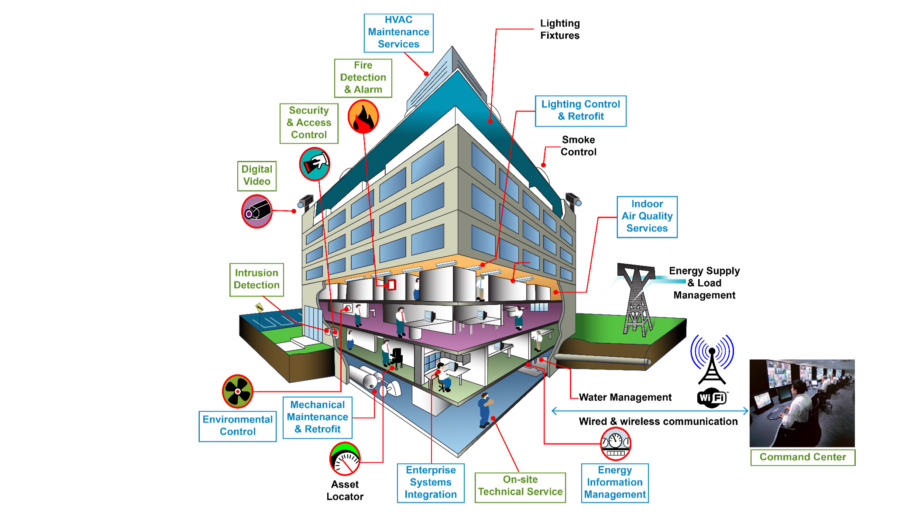
\includegraphics[width=0.9\textwidth]{figures/smart-building.jpg}
	\caption{Building Automation System schematic. Adapted from \cite{image-BAS}. }
	\label{fig:smart-building}
\end{figure}

The biggest problem in building automation is the market segmentation, where different manufactures created over the years different protocols and communication standards that didn't address solutions to all types of applications. This led to a more difficult and often impossible integration of this different approaches in the same system. Also, each vendor used to have closed specifications but, recently, in order to gain a higher margin of market, this specifications started being disclosed by vendors, which led to the appearence of new standards made from prior ones, combined. Presently the most used standards are BACnet, LonWorks, KNX and DALI. This different standards act in different \ac{bas} layers, which will be addressed in the next section. 

Though, with the rising of \ac{iot}, there have been an increasingly amount of new solutions that use high scalable technologies, well known communication standards, such as IP,  and use lightweight devices with low power consumption. This concepts will be addressed ahead in section 2.2.


\subsection{\ac{bas} Protocols}

In this section there will be addressed the most common technologies present at the current Building Automation market. Each one of them as an important role at different levels of a Building Automation System. As shown in Figure \ref{fig:hierarchy}, those levels are Management System Level, Automation Level and Field Level \cite{Iwayemi2011}. The all set of devices, sensors or actuators, compose the field layer. The Automation level is responsible for all the logic and hardware needed to control those devices and the Management Level consists in the control and management of the system and the reactions to events present in the gathered data.

\begin{figure}[H]
	\centering
	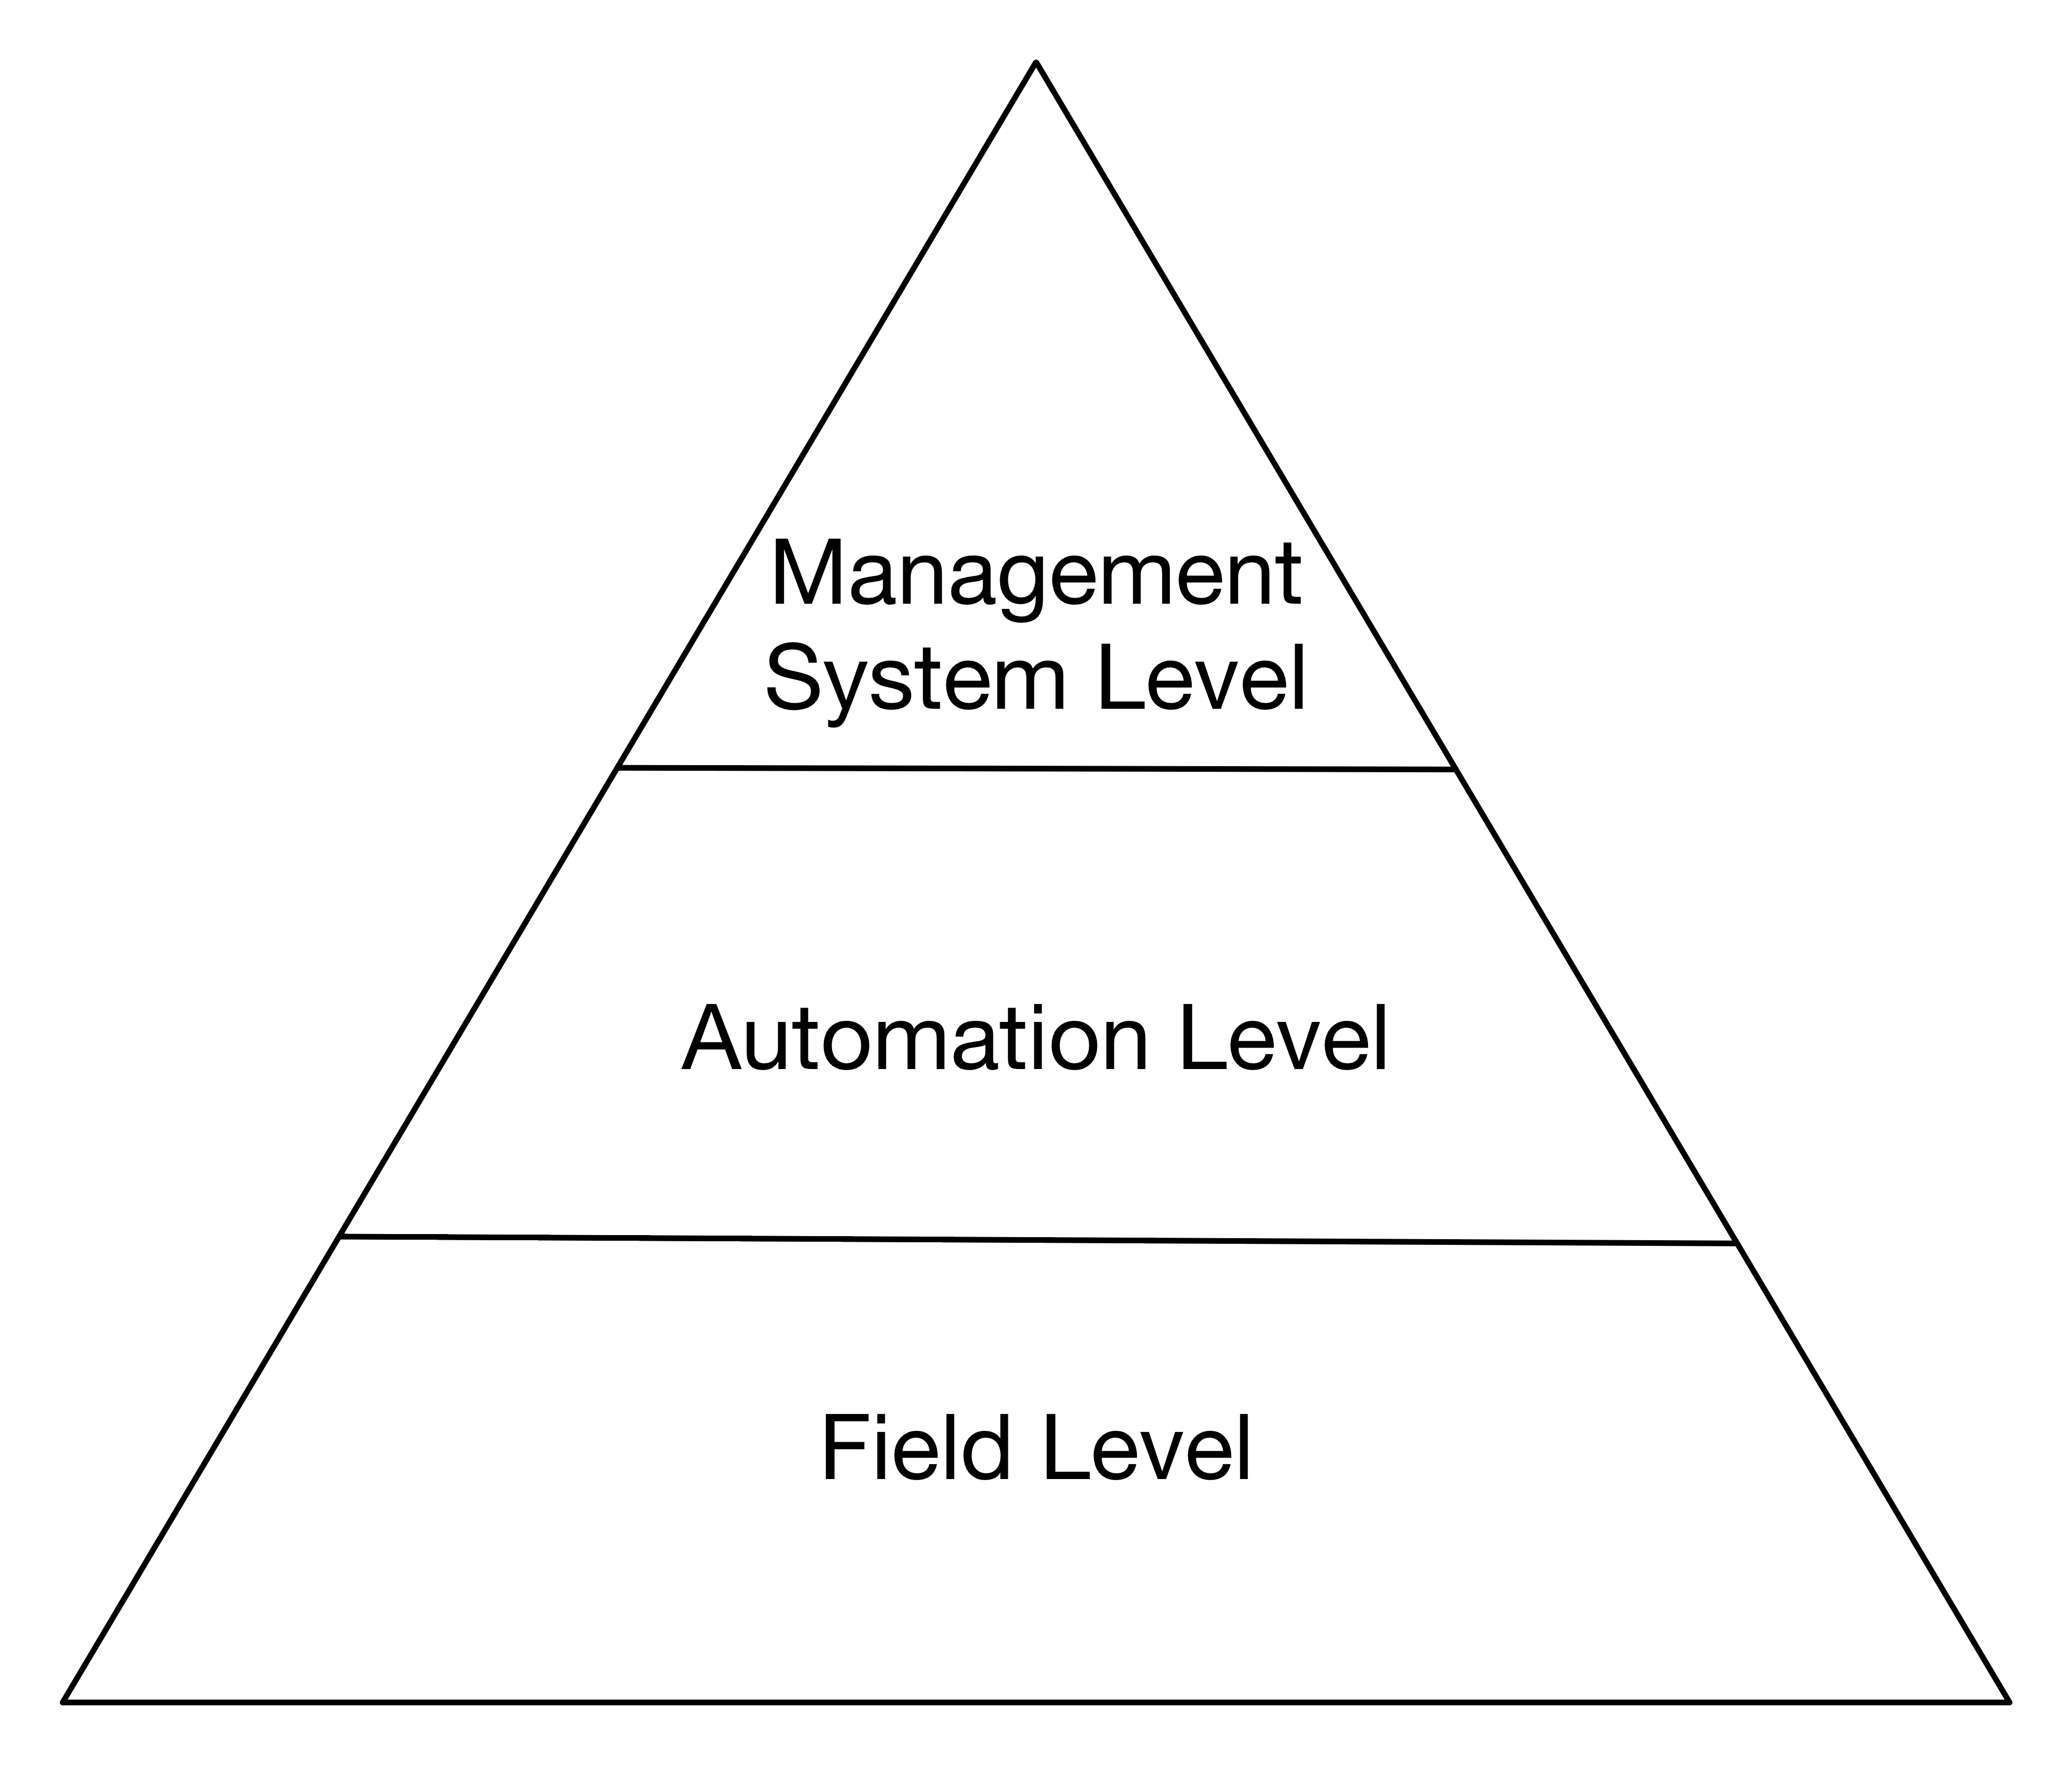
\includegraphics[width=0.9\textwidth]{figures/hierarchy.png}
	\caption{Building Automation System hierarchy \cite{kastener}. }
	\label{fig:hierarchy}
\end{figure}

The most common protocols used in BAS are \acf{bacnet} \cite{bacnet}, \acf{knx} \cite{knx}, \acf{lonworks} \cite{EchelonCorporation2009}, EnOcean \cite{enocean}, and \acf{dali} \cite{dali}. Each one of them has its own position on the \ac{bas} hierarchy. All the features of each one and the differences between them will be addressed in the next subsections.


\subsubsection{BACnet}
The \acf{bacnet} protocol, was developed by \acf{ashrae} in 1987 but was only published and accepted as a ANSI/ASHRAE standard latter in 1995.

\ac{bacnet} was designed to allow communication of building automation and control systems in fields such as HVAC, lighting control and others. The \ac{bacnet} protocol allow the deployment of automation mechanisms to sensors and actuators exchange information, irrespective of any service they perform.

\ac{bacnet} is modelled in object-oriented manner. There are a standard set object types that define the application services supported, such as devices, control loops, notifications, commands, schedules and more \cite{Domingues2016}. Each of the objects can have its own properties, that define together their functionality. For, example, a motion sensor can have multiple properties such as, number of times it was triggered and record of the last on-state time, and not only the current state. The access and manipulation of the object properties is done through a service that allows reading and writing object properties, that can interact with the real device state based on his object properties \cite{Fernbach2011}.

As stated before, other important \ac{bacnet} features are scheduling, which allow to schedule actions and program periodic events, notifications, that allow to distribute event notifications to the subscribed recipients \cite{Domingues2016} and logging, allowing a historical view of every change carried out in the system.

\ac{bacnet} is surely a complete solution that can be a good option for a full building automation system deployment. Yet \ac{bacnet} is an open standard, but the tools are supplied individually by each manufacturer \cite{openprotocol}, being sometimes complex the use and manage devices from different vendors. Figure \ref{fig:bacnet} shows an example of a multi vendor architecture.


\begin{figure}[H]
	\centering
	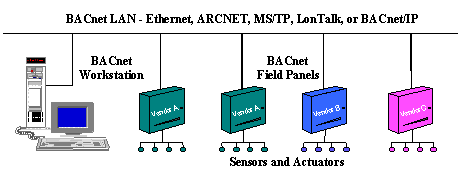
\includegraphics[width=0.9\textwidth]{figures/bacnet.png}
	\caption{Native BACnet architecture. Adapted from \cite{bacnetimage}. }
	\label{fig:bacnet}
\end{figure}


\subsubsection{KNX}

\ac{knx} was created from the combination of the best aspects of European Installation Bus (EIB), European Home Systems (EHS), and BatiBUS technologies. Later, KNX was standardized as norm EN 50090, and in 2006 as a international ISO/IEC 14543 standard \cite{Domingues2016}.

KNX deployment architecture uses a common bus connected to every device, actuator or sensor. The communication can be done using unicast addressing, since every device has a unique identifier corresponding to its position in the network. There is also the possibility of multicast communication since devices can be also aggregated in groups through a group identifier \cite{Kastner2005}.  

KNX support a variety of communication means such as twisted-pair (TP), power line (PL), IP tunnelling and a wireless one named KNX
Radio Frequency. Being KNX a field bus system \cite{Osorio}, the interworking of devices is a very important matter taken in account by KNX. This is possible since KNX certifies products in order to ensure that they apply to their interworking rules, such as, being able to communicate with the whole system, according to KNX specifications, and following the KNX standardized set of data types \cite{Interworking_KNX}. Also, KNX ensures that all the products can be configured using a Engineering Tool Software (ETS). This tool provides two modes of configuration, S-mode (System mode) and E-mode (Easy mode) as shown in Figure \ref{fig:knx_modes}. 

\begin{figure}[H]
	\centering
	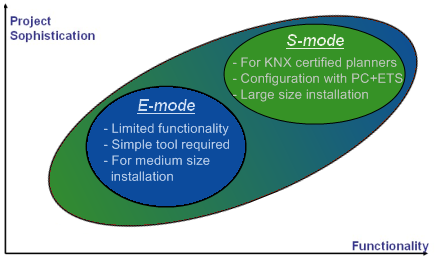
\includegraphics[width=0.9\textwidth]{figures/knx_modes.png}
	\caption{KNX configuration modes \cite{knx}. }
	\label{fig:knx_modes}
\end{figure}
 
 S-mode is intended to be used by experienced KNX installers as it offers full control over the system functions and configurations. The E-mode is targeted to installers with less experience, since components are already pre-programmed with a default array of parameters.
 
To conclude, KNX is capable of resolve most of the problems in the Building Automation field. Features such as the very rigorous certification program for devices from different manufactures is a great way to reduce the heterogeneity in communication between devices.

 
\subsubsection{LonWorks}

LonWorks is an event-triggered control network system \cite{Osorio}, developed by Echelon Corporation \cite{echelon} in 1988. This system uses LonTalk, a communication protocol firstly presented in 1999 as a official ANSI/EIA-709 standard and later as a ISO/International Electrotechnical Commission (IEC) 14908.

LonWorks uses a decentralized peer to peer architecture, where devices are treated as nodes and can communicate with each other by any medium available, using a standard protocol. This node's main component is a Neural Chip which is designed to provide intelligence and network communication capabilities to control devices. In addiction, this nodes have a unique identifier and a set of functionalities and network variables, i.e. all the datapoints needed to nodes communicate directly with each other \cite{Domingues2016}.

Also, the use of a standard network variable types (SNVT), facilitates integration, as it helps in the prevention of errors and simplifies the engineering process \cite{Siemens2013}. 


\subsubsection{DALI}
TODO

\subsubsection{EnOcean}
TODO

\subsection{\ac{bas} Solutions}
TODO

\subsubsection{HCL Technologies \ac{bas}}
TODO

\section{\acf{iot}}

\acf{iot} is a concept that have been emerging over the years in which in addition to the devices we usually connect to the Internet, like smartphones or personal computers, a new diversity of devices will also be connected, forming a vast network of smart objects. Devices like vehicles or normal household appliances will be equipped with sensors and actuators that will be able to gather data, giving people the information to do better and valuable decisions \cite{Weiser1991}. Also, with controllers and the sensing information, this devices can preform certain tasks without human intervention.

This concept was first introduced by Kevin Ashton \cite{Ashton} in 1999, where he stated his idea of having computers gathering information from things around us, that humans couldn't do by themselves, to give a new perspective to people of how to reduce waste, loss and cost. For this author, we needed to give computers the power to gather information with their own means, so they could sense the world for themselves and overcome the limited time, attention and accuracy humans have.

In the recent years, with the technological advances made in electronics, devices become smaller, low powered and more affordable, giving a boost to the integration of this concept in our society. According to \cite{Evans2011}, the turning point for \ac{iot} would be when there were more devices connected to the Internet than people. This point was reached somewhere between 2008 and 2009, and as can be seen in Figure \ref{iot_pic}, this numbers will grow exponentially in the next years and can even reach over a 5 to 1 factor between connected devices and the world population.

\begin{figure}[H]
	\centering
	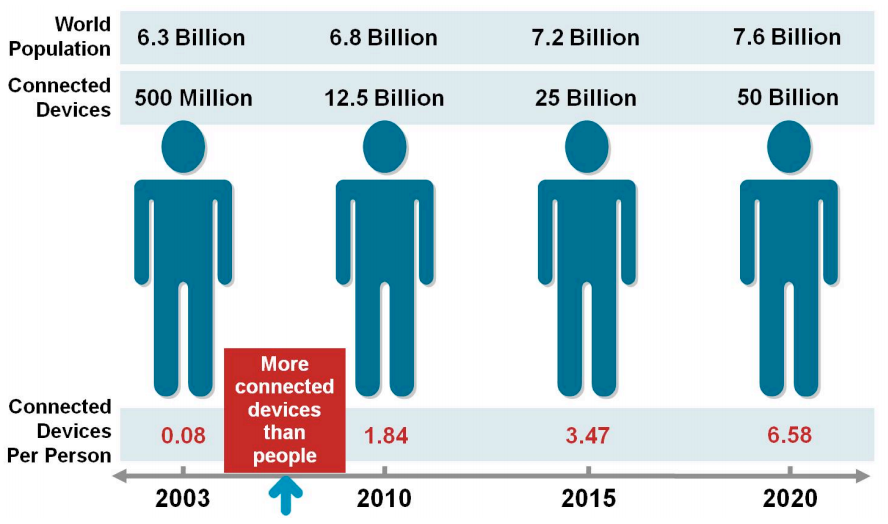
\includegraphics[width=0.9\textwidth]{figures/iot_pic.png}
	\caption{Estimated growth of connected devices \cite{Evans2011}. }
	\label{fig:iot_pic}
\end{figure}

Nevertheless, the growth of \ac{iot} still faces some challenges. As the authors of \cite{Al-fuqaha2015} state, with the grow number of devices being connected to the Internet, IPv6 is going to be crucial for the billions of new devices that will require for a unique IP address. The devices will also need to be self-sustainable with regard to energy consumption. Besides this factors, \ac{iot} remains with no agreements on what standards should be used, which is a problem since it hampers the communication between devices


The \ac{iot} concept, according to \cite{Evans2011} will be a very important evolution to the Internet, giving the ability to create new applications to improve people's lives. The sharing of knowledge and wisdom has always been a key factor for human evolution, and now, with \ac{iot} and the help of smart devices that sense, collect and share information, we can create new ways to enhance people's comfort and well-being.

To conclude, \ac{iot} will have an important role in a vast number of sectors, and example is \ac{bas}, where \ac{iot} has become a reference model and has helped to create new and more efficient solutions.



\subsection{\acf{m2m}}

\acf{m2m} term firstly emerged a few decades ago and it was used in telemetry, industrial and automation systems \cite{}. Nowadays it is often associated with \ac{iot}, since it refers to the exchange of information between machines, in order to preform tasks and actions without human intervention.

Although both of the concepts goals remain alike, i.e. enable communication between machines, \ac{m2m} should be considered as a subset of \ac{iot}, as it lacks in the creation of meaning to the information exchanges. \ac{iot} is a wide web of not only \ac{m2m} networks but also, a vast set of applications that enables, as stated in the previous section, automatic decision making and data analytics. 

\subsection{\acf{wsn}}

\acf{wsn} is a network of distributed devices, sensors and/or actuators, interconnected by a wireless medium. As stated in \cite{IEC2014a}, this network of nodes sense and control the environment cooperatively, enabling the interaction between persons or computers and the environment around them. 

Nowadays \ac*{wsn}s usually include sensors, actuators and gateways. Sensors are devices capable of detecting changes in environmental variables and supply that information to other nodes. This devices can measure variables like luminosity, temperature, humidity, pressure, motion and a wide variety of other environmental data. Actuators, in the other hand, are devices that control mechanisms to alter the physical environment state and preform this actions based on input data. For instance, an actuator can be programmed to turn on or off a air conditioner based on a input trigger set off by the temperature in a room.
Lastly, gateways are devices connected to sensors and actuators, responsible orchestrate and interconnect this devices, as well as for mechanisms of automation and remote access. Gateways can be programmed to based on input data gathered by sensors and a set of pre loaded rules, trigger a actuator to act on some physical environment element. Gateways are the brains of \ac{wsn}s. Also, gateways can be programmed with self learning mechanisms and autonomously control devices. 

The connection between this three devices form a \ac{wsn}, which is, nowadays, the primary enabler of \ac{iot}, since, with the use of \ac{iot} protocols and standards, this nodes become smart objects. In the following sections, this \ac{iot} protocols will be discussed.




\subsection{Wireless Communication Protocols}

The communication between devices is one of the most important concerns of \ac{iot}. The devices must be able to communicate with each other, through standardized protocols, in other to achieve full interoperability between them. 

In this section there will be presented some of the most used communication protocols in \ac{iot}. Since \ac{iot} devices will need to have wireless networking capabilities and be battery-powered, the main focus for this section will be wireless protocols with low power usage for the devices.

When talking about wireless communication, the protocol that first comes to mind is IEEE 802.11, better known as Wi-Fi. This wireless standard was introduced in 1997 by the \acf{ieee} \cite{Bellis2017}, and nowadays it's used across all laptops, phones and other media devices. Although it has an important role for this kind of technological equipments, IEEE 802.11 has never been widely used for communication between \ac{iot} devices. The reason for that is the heavy power requirements that such protocol need, making it unsustainable for smart devices to use it.

Another important and well known wireless protocol for communications between devices is Bluetooth. This standard was created in 1999 by \acf{sig} and in 2016 reached its fifth version \cite{BluetoothSIG2016}. Bluetooth is widely used for connecting smartphones to other bluetooth enabled devices, such as wearables, cars and others, making it one of the most used close range communication protocol.

Both Bluetooth and Wi-Fi standards have polished and mature specifications, making them reliable communication protocols. However this standards are not suited for low capabilities devices since they were not created with restrictions like low power consumption and limited resources in mind. Over the next sections, will be presented a variety of protocols, more suited for this kind of devices.

\subsubsection{IEEE 802.15.4}

The IEEE 802.15.4 standard was introduced by the \acf{ieee} and its intent was to target Low Rate WPANs (LR-WPANs) \cite{Kemp2010}. This protocol specifies the two lowest layers of the OSI model, represented in Figure \ref{fig:osi}, and it is branded for its simpleness, low data rates and battery saving \cite{Devadiga2003}.

\begin{figure}[H]
	\centering
	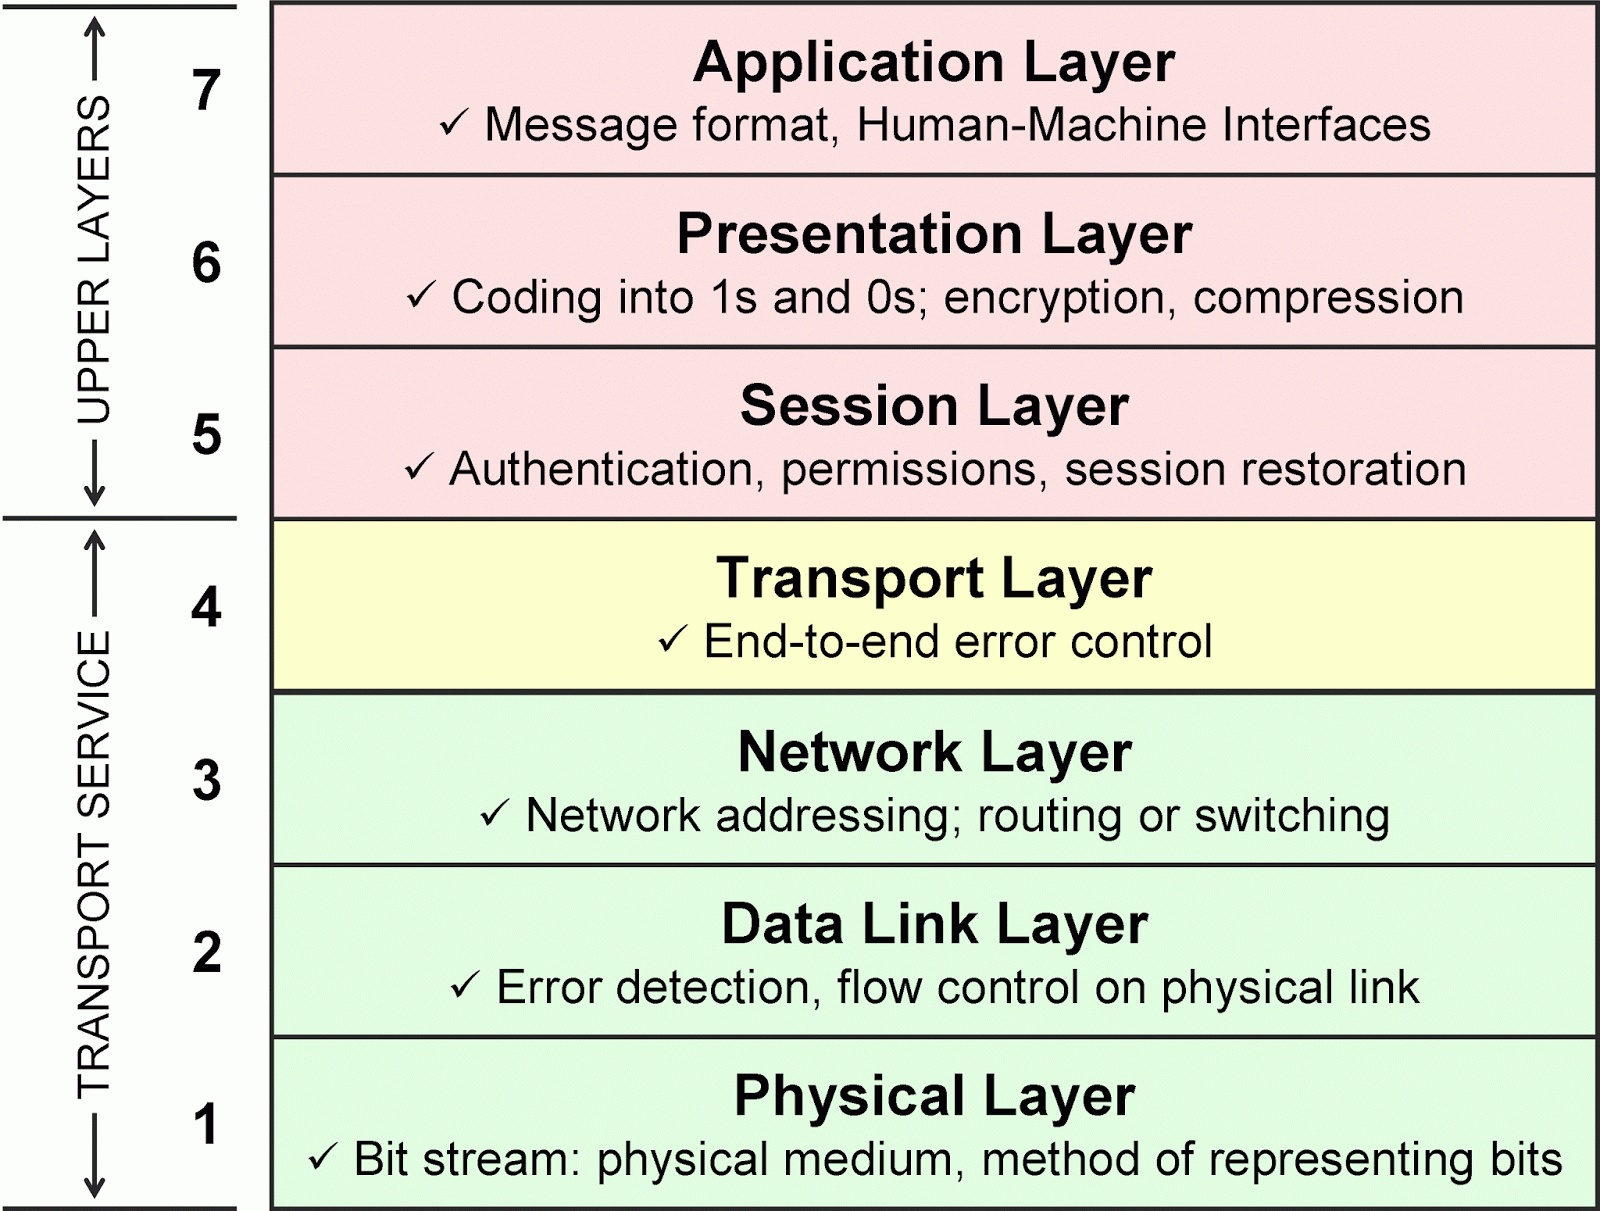
\includegraphics[width=0.7\textwidth]{figures/osi.png}
	\caption{\acf{osi} model \cite{Zikrillah}.}
	\label{fig:osi}
\end{figure}

This characteristics are what make this standard quite significant for \ac{iot}. Since \ac{iot} sensors and actuators have many battery constrains, using a protocol that has this facts in mind, make IEEE 802.15.4 a suitable standard for communications within \ac{wsn}s.

IEEE 802.15.4 is also the baseline for other \ac{iot} communication protocols such as ZigBee, which will be covered in a section below.


\subsubsection{6LoWPAN}
TODO
\subsubsection{ZigBee}
TODO
\subsubsection{\acf{ble}}
TODO
\subsubsection{IEEE802.11ah}
TODO
\subsubsection{Wireless Communication Protocols Comparison}
TODO
\subsection{Application Protocols}
TODO
\subsubsection{\acf{mqtt}}
TODO
\subsubsection{\acf{amqp}}
TODO
\subsubsection{\acf{coap}}
TODO
\subsubsection{\acf{xmpp}}
TODO
\subsubsection{Interaction Protocols Comparison}
TODO

\section{Fault Tolerance}
TODO

\subsection{Fail mechanisms in \ac{bas} }
TODO




	\chapter{Smart Building Solution}
\label{chapter:architecture}

In this chapter there will be provided a solution to improve the efficiency and usability of a building by using automation mechanisms, enhancing the intelligence of the building. Taking in account the \ac{iot} principles, this system should be capable of real-time processing of large data streams, analyse and correlate events, and being able to react and adapt to emergency states and guarantee the minimum functionality, always. This solution is intended to integrate the SmartLightinhg project and will be addressed in this chapter.

This chapter will begin with a brief description, in section \ref{Architecture:slproject}, of SmartLighting project and its intentions of developing a smart environment of automation and control in IT2 building. Later, in order to ensure that all system necessities are addressed and taken into account, in section \ref{Architecture:Requirements} will be done a survey of necessary capabilities and  requirements to satisfy its stakeholders.

Since the main aim of this dissertation is the failure handling and adaptation of the gateways to emergency states, in section \ref{Architecture:usecases}, will be addressed three scenarios of operation needed to be taken into account.

Finally, in section \ref{Architecture:Architecture}, a presentation and evaluation of the system architecture, and its components interactions. 


\newpage


\section{SmartLighting Project}
\label{Architecture:slproject}

\subsection{Project Overview and Objectives}
\label{Architecture:Overview}

The SmartLighting project\cite{Moreira} aims to create a smart environment in IT2 building in order to automate the lighting and HVAC infrastructure. IT2 building have been running with CFL luminaries, which, are often not only, inefficient and hazardous for the environment, but also, in most cases, unable to be dimmed. 

This project intend to remove all this CFL luminaries by LED luminaries, that can resolve all the issues stated before and also are able, combining with sensors, to collect data from the environment such as luminance, temperature, humidity, motion and others. All of the collected data will be used to act in real-time to the changes in sensors readings. 

Such system needs to be backed up by an intelligent management platform in order to act based on a set of rules and input streams of sensors values. Moreover, there will be mechanisms to correlate events and determine patterns that will enable a more immediate reaction. As an example, if a user has the habit of turn on the AC everyday in the morning, the system will be able to learn and automatically do that action soon as the user arrives in the building. 

Also, the system can use external sources such as meteorological forecast to take preventively actions, such as increase the dimming levels of luminaries and the building temperature in cold rainy days.

Additionally, the users will be able to set their own rules to enhance the comfort in its office. This can be done either by using a mobile application or a web interface. Also, this user platforms can enable the use of notifications providing ways to alert the building occupants of important events. For instance, users can be informed about future meetings, the presence of another occupant in the building, and more.

Finally, an important feature for this project is the fail safe mechanisms to ensure that all the basic automation needed for the building well functioning, such as the trigger of a motion sensor lighting up the corresponding luminaries, work even if in situations of failure in core elements of the architecture or network communication problems. This can be achieved by giving gateways, the component that communicate directly with the sensors and actuators, lightweight processing mechanisms to ensure the basic functionalities described before. This will be the main focus of the presented dissertation.



\subsection{Stakeholders}
\label{Architecture:Stakeholders}

The success of a project depends directly in the people involved, either by developing its features or simply by consuming them in its final form. A correct identification of the stakeholders, their motivations and expectations, pay a important role in the success of any project. 

In SmartLighting project, 4 stakeholders were identified, namely:

\begin{itemize}
	\item Building occupants
	\item Building owners
	\item Building managers
	\item Developers team
\end{itemize}


The primary stakeholders in this project, are the IT2 building occupants and owners. While occupants will take direct advantage from the implemented features due to the enhance in comfort and usability of the building, owners gains will be economic as far as the building energy consumption and maintenance costs will be reduced.

As for building managers, the benefits are from easier interaction and configuration of the whole system, that allow a more precise aware of every node status, to a notification system for quicker reaction to system failures, or even to prevent such ones, and act before they happen.

Lastly, the developers team take a huge benefit in the success of the project since they are interested and devoted to create the best product possible that fulfils all the other stakeholders expectations.


\subsection{Use Cases}
\label{Architecture:SLusecases}

Based on the stakeholders survey done previously, the two main actors for this \ac{bas} solution are the building's manager and the occupants. Those actors directly use the platforms and resources provided, to enhance the comfort of the environment around them as they please, so the main focus for user driven cases will be in those two. 

Although there are many use cases for both the building's manager and the occupants, in this section will be only addressed those that were already implemented in this project, giving a greater understanding of the overall project's functionalities. Later in section \ref{Architecture:usecases}, there will be presented the use cases and scenarios introduced by this dissertation work.

\begin{Paragraph}{Building occupant}
	
The building occupants will be the principal users that will interact with the system. This interaction can be achieved by using either a mobile application or a web interface. The use cases addressed bellow combine the most common and frequent operations:


\begin{figure}[H]
	\centering
	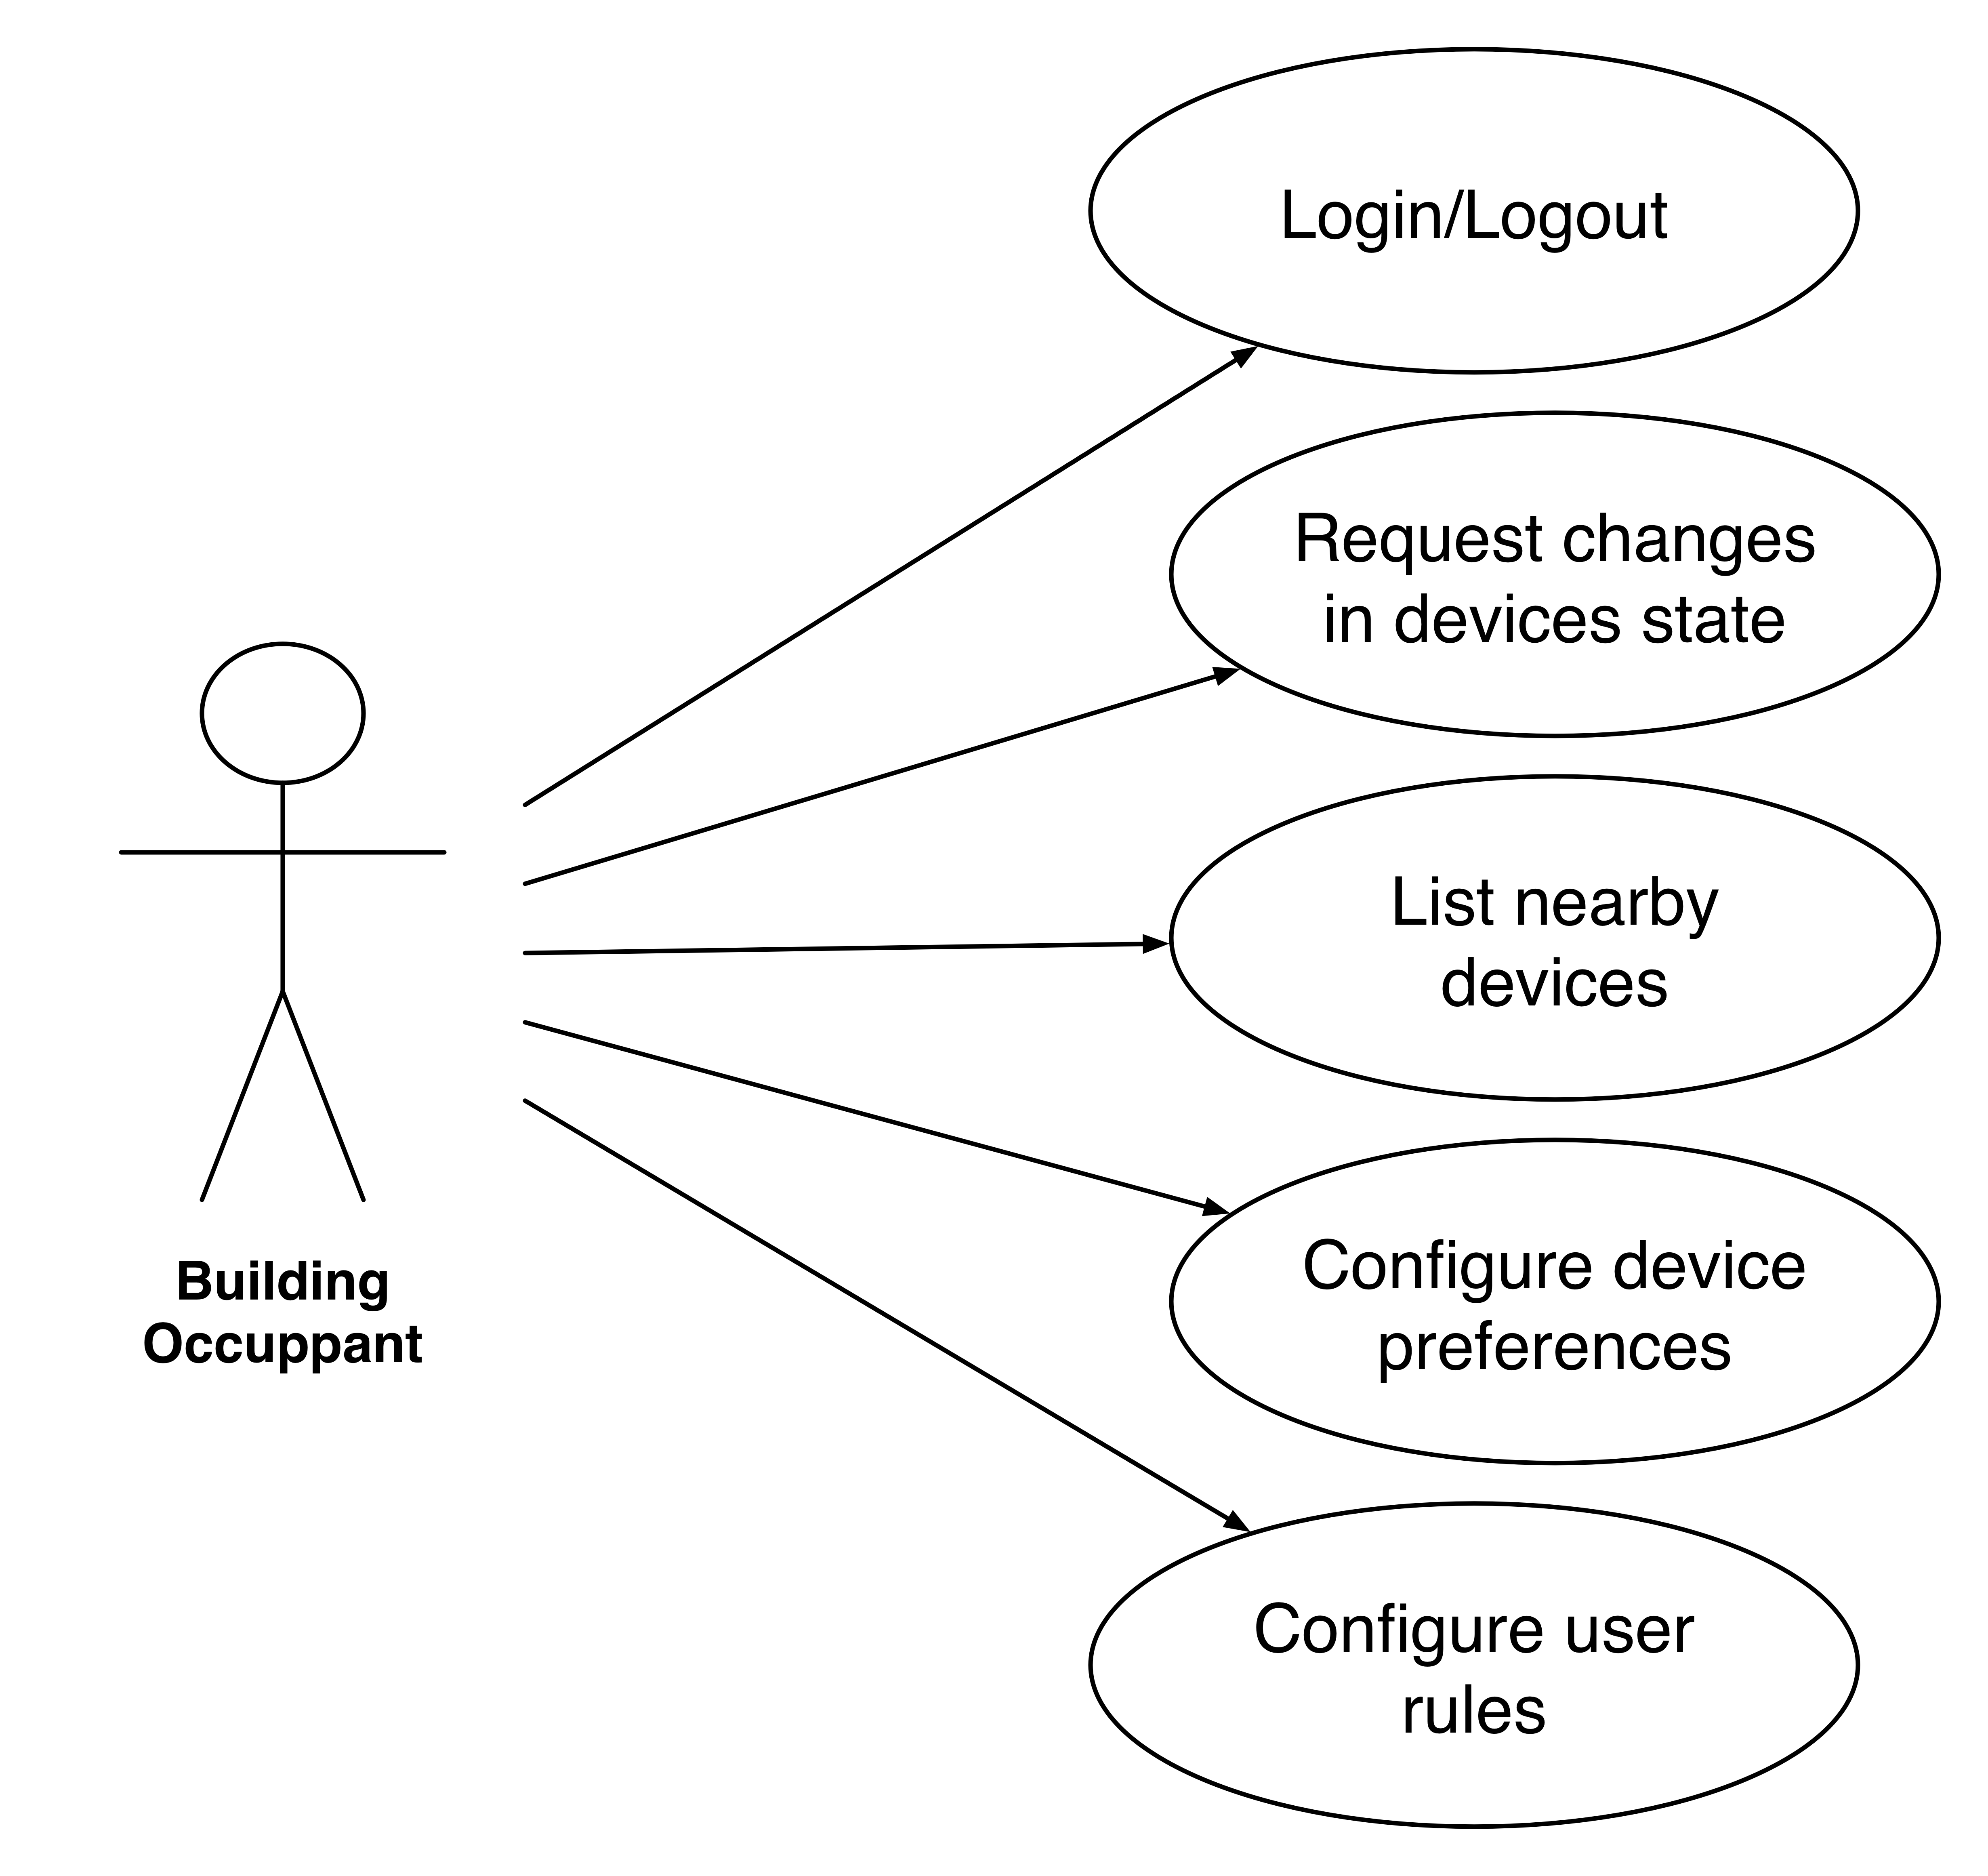
\includegraphics[width=0.5\textwidth]{figures/usecase1.png}
	\caption{Use case diagram of building occupants interaction with the system.}
	\label{fig:user}
\end{figure}

\begin{itemize}

	\item{\textbf{Login/Logout:}	This use cases are intended to enable the access to user oriented features. The building occupants can login in the platform, either using the mobile application or the web interface, to access his preferences and personal environment control features.}
	\item{\textbf{Request changes in devices state:}	The building occupant can request a change in the state of a device, that can be accepted or denied by the system depending on the access rights of the user. For instance, an occupant can request a change in near by devices like  air conditioners, lights, and others.}
	\item{\textbf{List nearby devices:}	This use case allows users to request the list of nearby devices, based on its location, allowing to access or request changes to devices in the same room as the occupant, giving that these are the most likely to be needed access.}
	\item{\textbf{Configure device preferences:}	The user can create or edit device pre-sets, allowing that the selected values are applied automatically to the device in future uses. For instance, the air conditioner in a user office can be pre-set to 21ºC so that when this device is turned on, that value is automatically set. This changes would also depend with the user access rights.}
	\item{\textbf{Configure user rules:}	This use case allow the building occupants to create rules that preform a set of actions automatically, giving the right conditions. For instance the user could create a rule to automatically turn the air conditioner on if the temperature in his office exceed a giving value.} 

\end{itemize}
\end{Paragraph}


\begin{Paragraph}{Building manager}
	
	
	\begin{figure}[H]
		\centering
		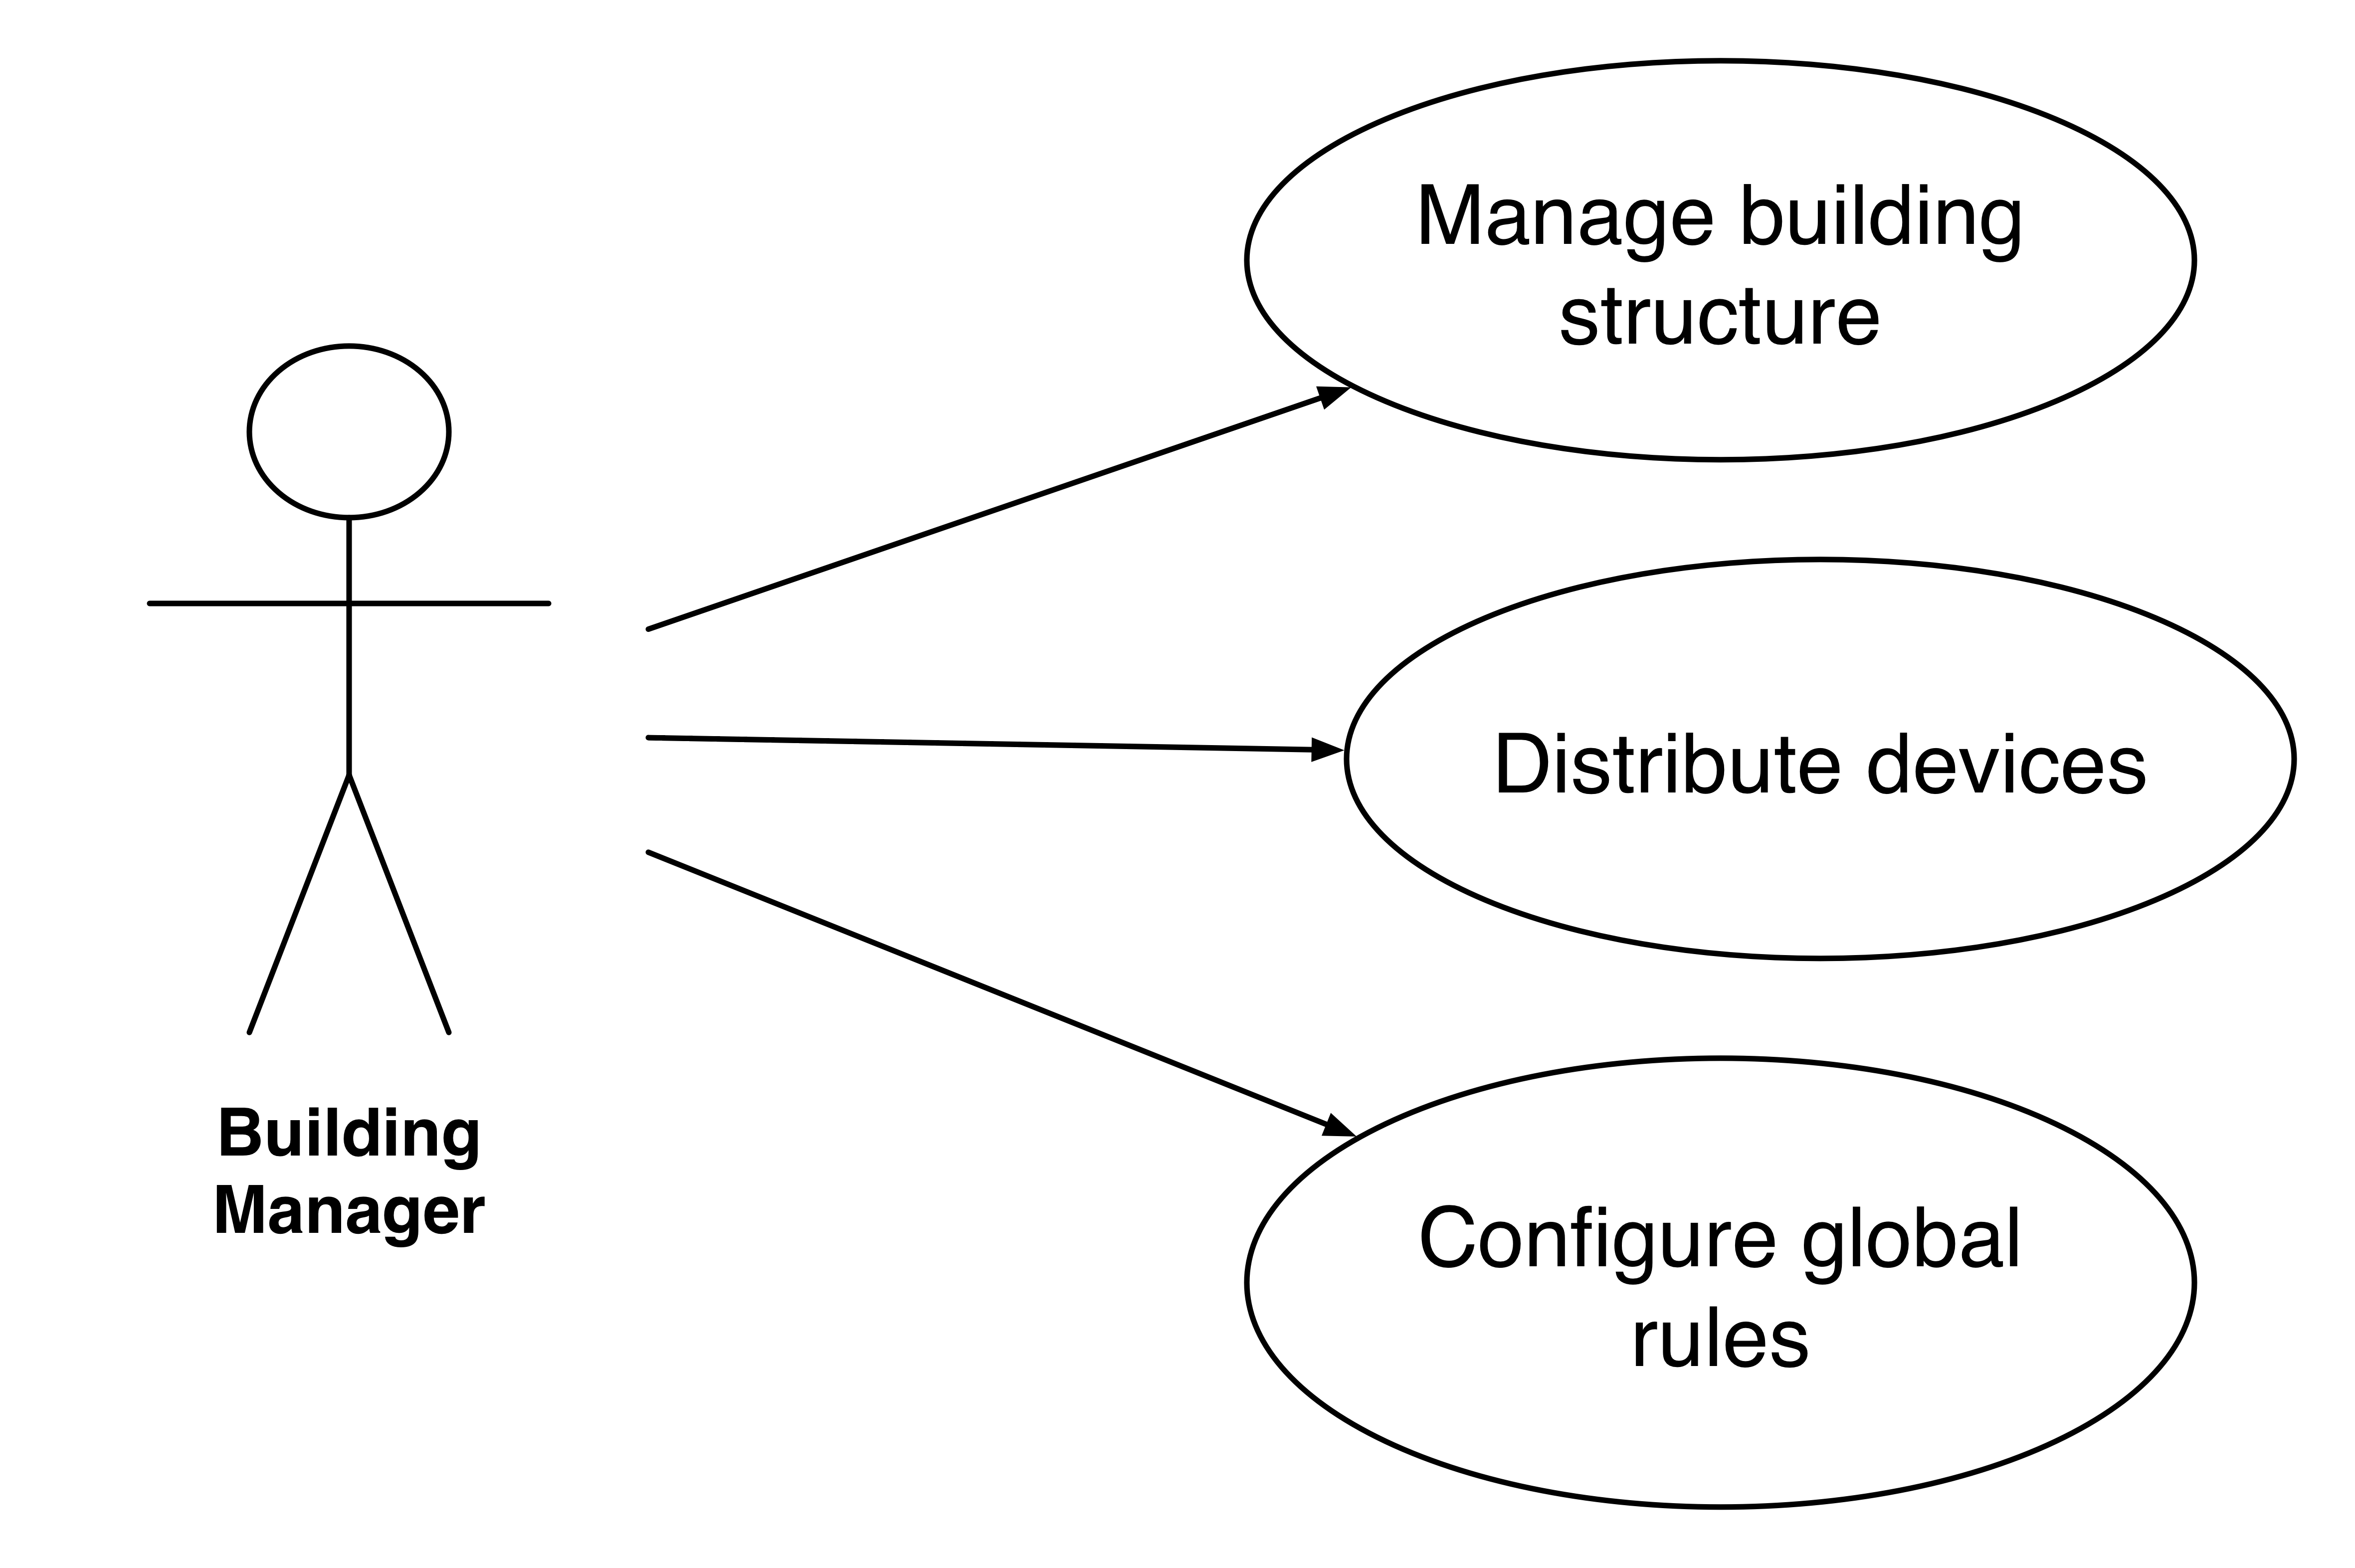
\includegraphics[width=0.5\textwidth]{figures/usecase2.png}
		\caption{Use case diagram of building manager interaction with the system.}
		\label{fig:manager}
	\end{figure}
\begin{itemize}
	\item{\textbf{Manage building structure:}	The manager can create the representation of the building in the structure management platform. This allow the creation of a virtual portrayal of the floors, rooms and areas of the building.}
	\item{\textbf{Distribute devices:}	This use case permit that connected devices can be distributed through the areas and rooms of the building virtual representation.}
	\item{\textbf{Configure global rules:}	The building manager has the ability to add, delete, enable or disable rules for the whole building. These core rules' main purpose are the building's efficiency increase, for instance instead of leaving the corridors lights always on, a rule can be created to turn them off when there's no one walking by. There is also a mechanism to test the rule before the deployment.}
\end{itemize}
\end{Paragraph}


\section{System Architecture}
\label{Architecture:Architecture}


Taking into account the objectives for this dissertation, and the existing architecture for the SmartLighting project, the proposed architecture has in mind, not only \ac{iot} and complex event processing principles, but also the referred features for this dissertation such as failure handling and rules distribution through gateways.

In this section will be presented the global system architecture for this project, represented in Figure \ref{fig:arch} as well as a description of all the components that compose the solution.

Note that components like the \ac{cep} engine, and the \ac{bm} are already implemented due to a past dissertation for the SmartLighting project \cite{helder}.

\begin{figure}[H]
	\centering
	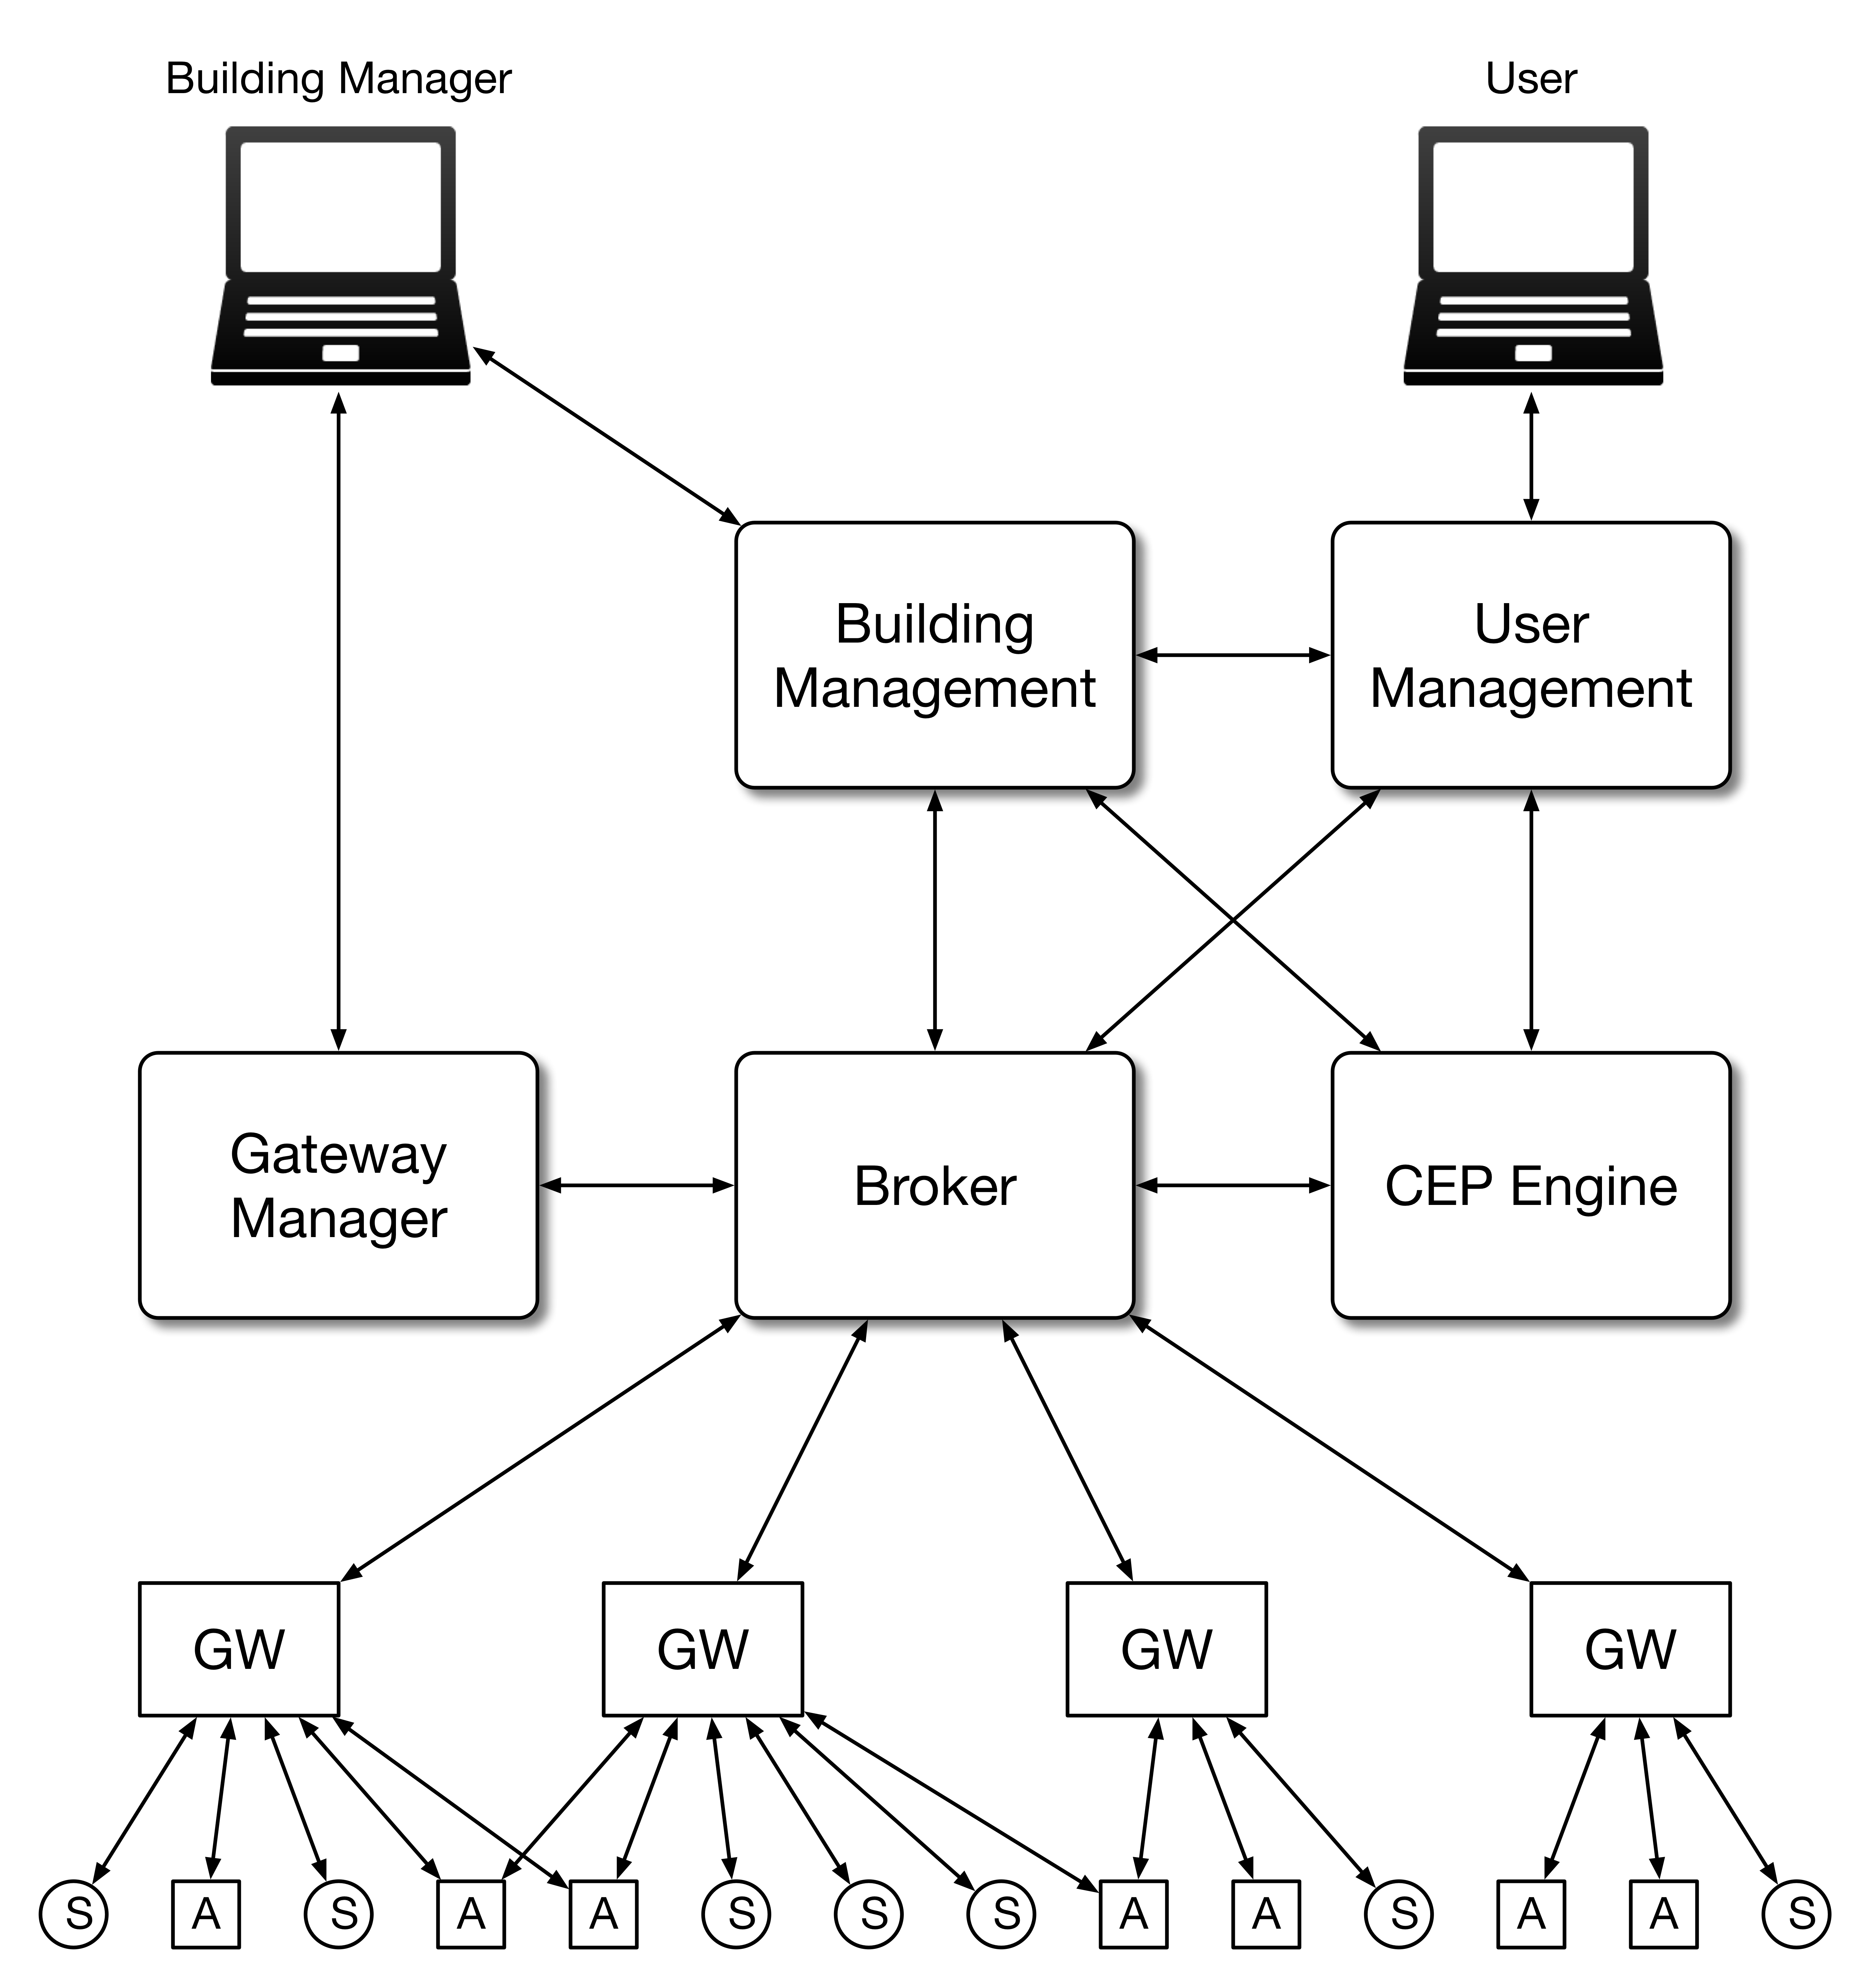
\includegraphics[width=0.9\textwidth]{figures/architecture.png}
	\caption{Smart Building: Architecture diagram}
	\label{fig:arch}
\end{figure}



\subsection{Components Overview}

\begin{Paragraph}{User Management}
	
	The user management platform is responsible for giving to common users of the building, the ability to interact with the platform through a web page. Users can manage their own building rules and control field devices directly. This can be done by publishing on the broker the wanted changes or by communication directly with the CEP Engine or the building management platform.
	
\end{Paragraph}

\begin{Paragraph}{Building Management}
	
	The building manager component is a user friendly platform that aims to facilitate the rule management and the configuration of the building's schema. The building manager can create, edit  or delete rules in a simple intuitive way and this component later translates them in a complex language that the CEP Engine can understand. Also, through a virtual representation of the building, the \ac{bm} can distribute devices across all its areas. After the correct configuration of the desired devices, this component is responsible for providing the information about each device and how should the CEP engine, and the other blocks of the architecture, address to this device in order to, for instance, send an order to change state or report new sensor data to the CEP Engine.
	
\end{Paragraph}

\begin{Paragraph}{CEP Engine}
	
	The CEP Engine is one of the most important components for a successful building automation solution. This engine must be a real-time and high performance component, that should be able to process hundreds of sensor triggered events per second based on complex rules created by the users. The actions preformed by this engine can be either directly to an actuator or to a component in the platform. For instance, sending an alert to the building manager when there are irregular sensor readings.
	
	
\end{Paragraph}

\begin{Paragraph}{Broker}
	
	The broker component, which refers to a message broker, it is responsible for receive and route information across the connected components. Every component connects to receive and send information, to and from other components.
	
\end{Paragraph}

\begin{Paragraph}{Gateway Manager}
	
	The gateway manager is the component responsible for rules distribution to gateways and fail handling. The first one, since gateways will be equipped with the ability to process events, based on simple rules in the case of CEP failure, there is the need for a regulator to distribute and be always aware where this rules are being deployed, and, in case of a gateway failure, distribute the devices and rules from that gateway, to other ones capable of supporting them. Also, the gateway manager should guarantee a balanced number of rules and devices across all gateways. For instance, if two gateways are in the reach of the same device, the gateways manager should allocate that device to the gateway with fewer devices.
	
	
\end{Paragraph}

\begin{Paragraph}{Gateways}
	
	Gateways are responsible for discovering devices and communicate to them. This nodes have to convert sensor's events into understandable messages to the automation engine, and vice versa. Also, gateways should be equipped with a lightweight automation engine so that, in case of a failure in the CEP Engine or in the broker, the gateways can continue to process events, and thus, a minimum downtime in the system's functioning.
	
\end{Paragraph}

\begin{Paragraph}{Sensors and actuators}
	
	The field layer represents the set of devices, both sensors and actuators, used to gather information and interact with the environment. The information gathering and detection of changes is done by sensors, that send this information to the respective gateways in the Network layer. After the processing of this data, either in the Aggregation and Automation layer or even by the gateways in the Network layer, the orders for changes are sent to the actuators.
	
\end{Paragraph}

\section{Requirements}
\label{Architecture:Requirements}
As stated before, the proposed solution for this dissertation is part of the SmartLighting project, thus, designed to be integrated in a real-world scenario. Accordingly, the requirements, in this section, must converge and be in conformity with the project's objectives stated in section \ref{Architecture:slproject}. 

\begin{Paragraph}{Fast Responsiveness}

The system's performance and fast responsiveness are huge requirements for a successful \ac{bas} solution. The system must react to events with such responsiveness that the occupants experience and comfort is not affected. For instance, when a user enters a room, it is expects that the lights turn on in a question of milliseconds causing an instantaneousness feeling to the user. In other cases, a slower responsiveness is not critical for the occupant. As an example, in the heating system, when the temperature goes bellow a certain threshold, if the air conditioners take a few seconds to turn on, it won't be noticeable for the users.

In addiction, the system's management platform responsiveness is another performance requirement as it shouldn't feel slow to the user.

\end{Paragraph}

\begin{Paragraph}{Flexibility}

One important requirement for this project is flexibility. Firstly, in order to have a system that can be easily upgradable, components must be independent of hardware. For instance, the gateway software must be developed in such way that can work in a large number of micro-controllers and  low power \ac{soc} computer. Also, the communication protocols between system components should be able to be changed allowing to meet different requirements of different scenarios. 


Finally, the system should facilitate the integration of different type of sensors or actuators, without the need verbose and difficult configurations.

\end{Paragraph}

\begin{Paragraph}{Scalability}

The system should assure that with the addition of devices, the overall performance does not decline. Also, it should facilitate the horizontal scalability of system nodes, making it transparent and easy to integrate new servers to maintain or improve the system's performance.

\end{Paragraph}

\begin{Paragraph}{Failure Handling and Basic Functionalities}
	
Failure handling and the assurance of basic functionalities were the main goals for this dissertation, making very important, the requirements regarding this topic.

The whole system is designed to fulfil a set of expectations and to work perfectly at any given time, however, there could be some cases where due to a critical system failure, either a downtime in the CEP engine, communication errors or a congested network, the whole system could start malfunctioning. In more severe cases this could mean, for instance, an entire blackout in a building, or a fire sensor not triggering the alarm leading to serious injuries to the occupants.

With all this facts in consideration, a significant requirement for a \ac{bas} solution is the ability to be always aware of the entire system state and to react immediately to abnormal system occurrences. This means, for instance, that in case of communication failure between the sensors and the \ac{cep} engine, the basic functionalities like lights turning on or off, alarms, doors and other key functionalities still work autonomously.
\end{Paragraph}

\begin{Paragraph}{Data Correlation}

In order to a more accurate and elaborate reaction to sensing events, the event processing unit should be able to correlate events and infer decisions based on previous learning. For instance, if a user always turn on the air conditioner, when the temperature is bellow a certain threshold, the system should be able to learn from this behaviour and promptly react without human intervention.

\end{Paragraph}

\begin{Paragraph}{User Control and User-friendly Interfaces}
	
The system should allow users, based on their roles and permissions, to manually alter the state of a device. This means that interfaces, web or mobile, should be available to the users to control the surroundings. This interfaces should be done, taking in account that not all users have the expertise to interact with verbose configuration parameters, thus, the interfaces should be as intuitive and perceptible as possible.
	
\end{Paragraph}




\section{Failure Use Cases}
\label{Architecture:usecases}

In order to achieve an environment where the minimum functionality of the system is always assured, for example, the lights turning on when someone walks in a corridor, there can be no system component that, in case of failure, could put in risk those functionalities. With this in mind, and looking to the existing architecture, simplified in Figure \ref{fig:sc1} only with components that directly and actively affect the event processing capability, three operation scenarios can be identified. 


\begin{Paragraph}{Scenario 1 - All components are operational}
	
	\begin{figure}[H]
		\centering
		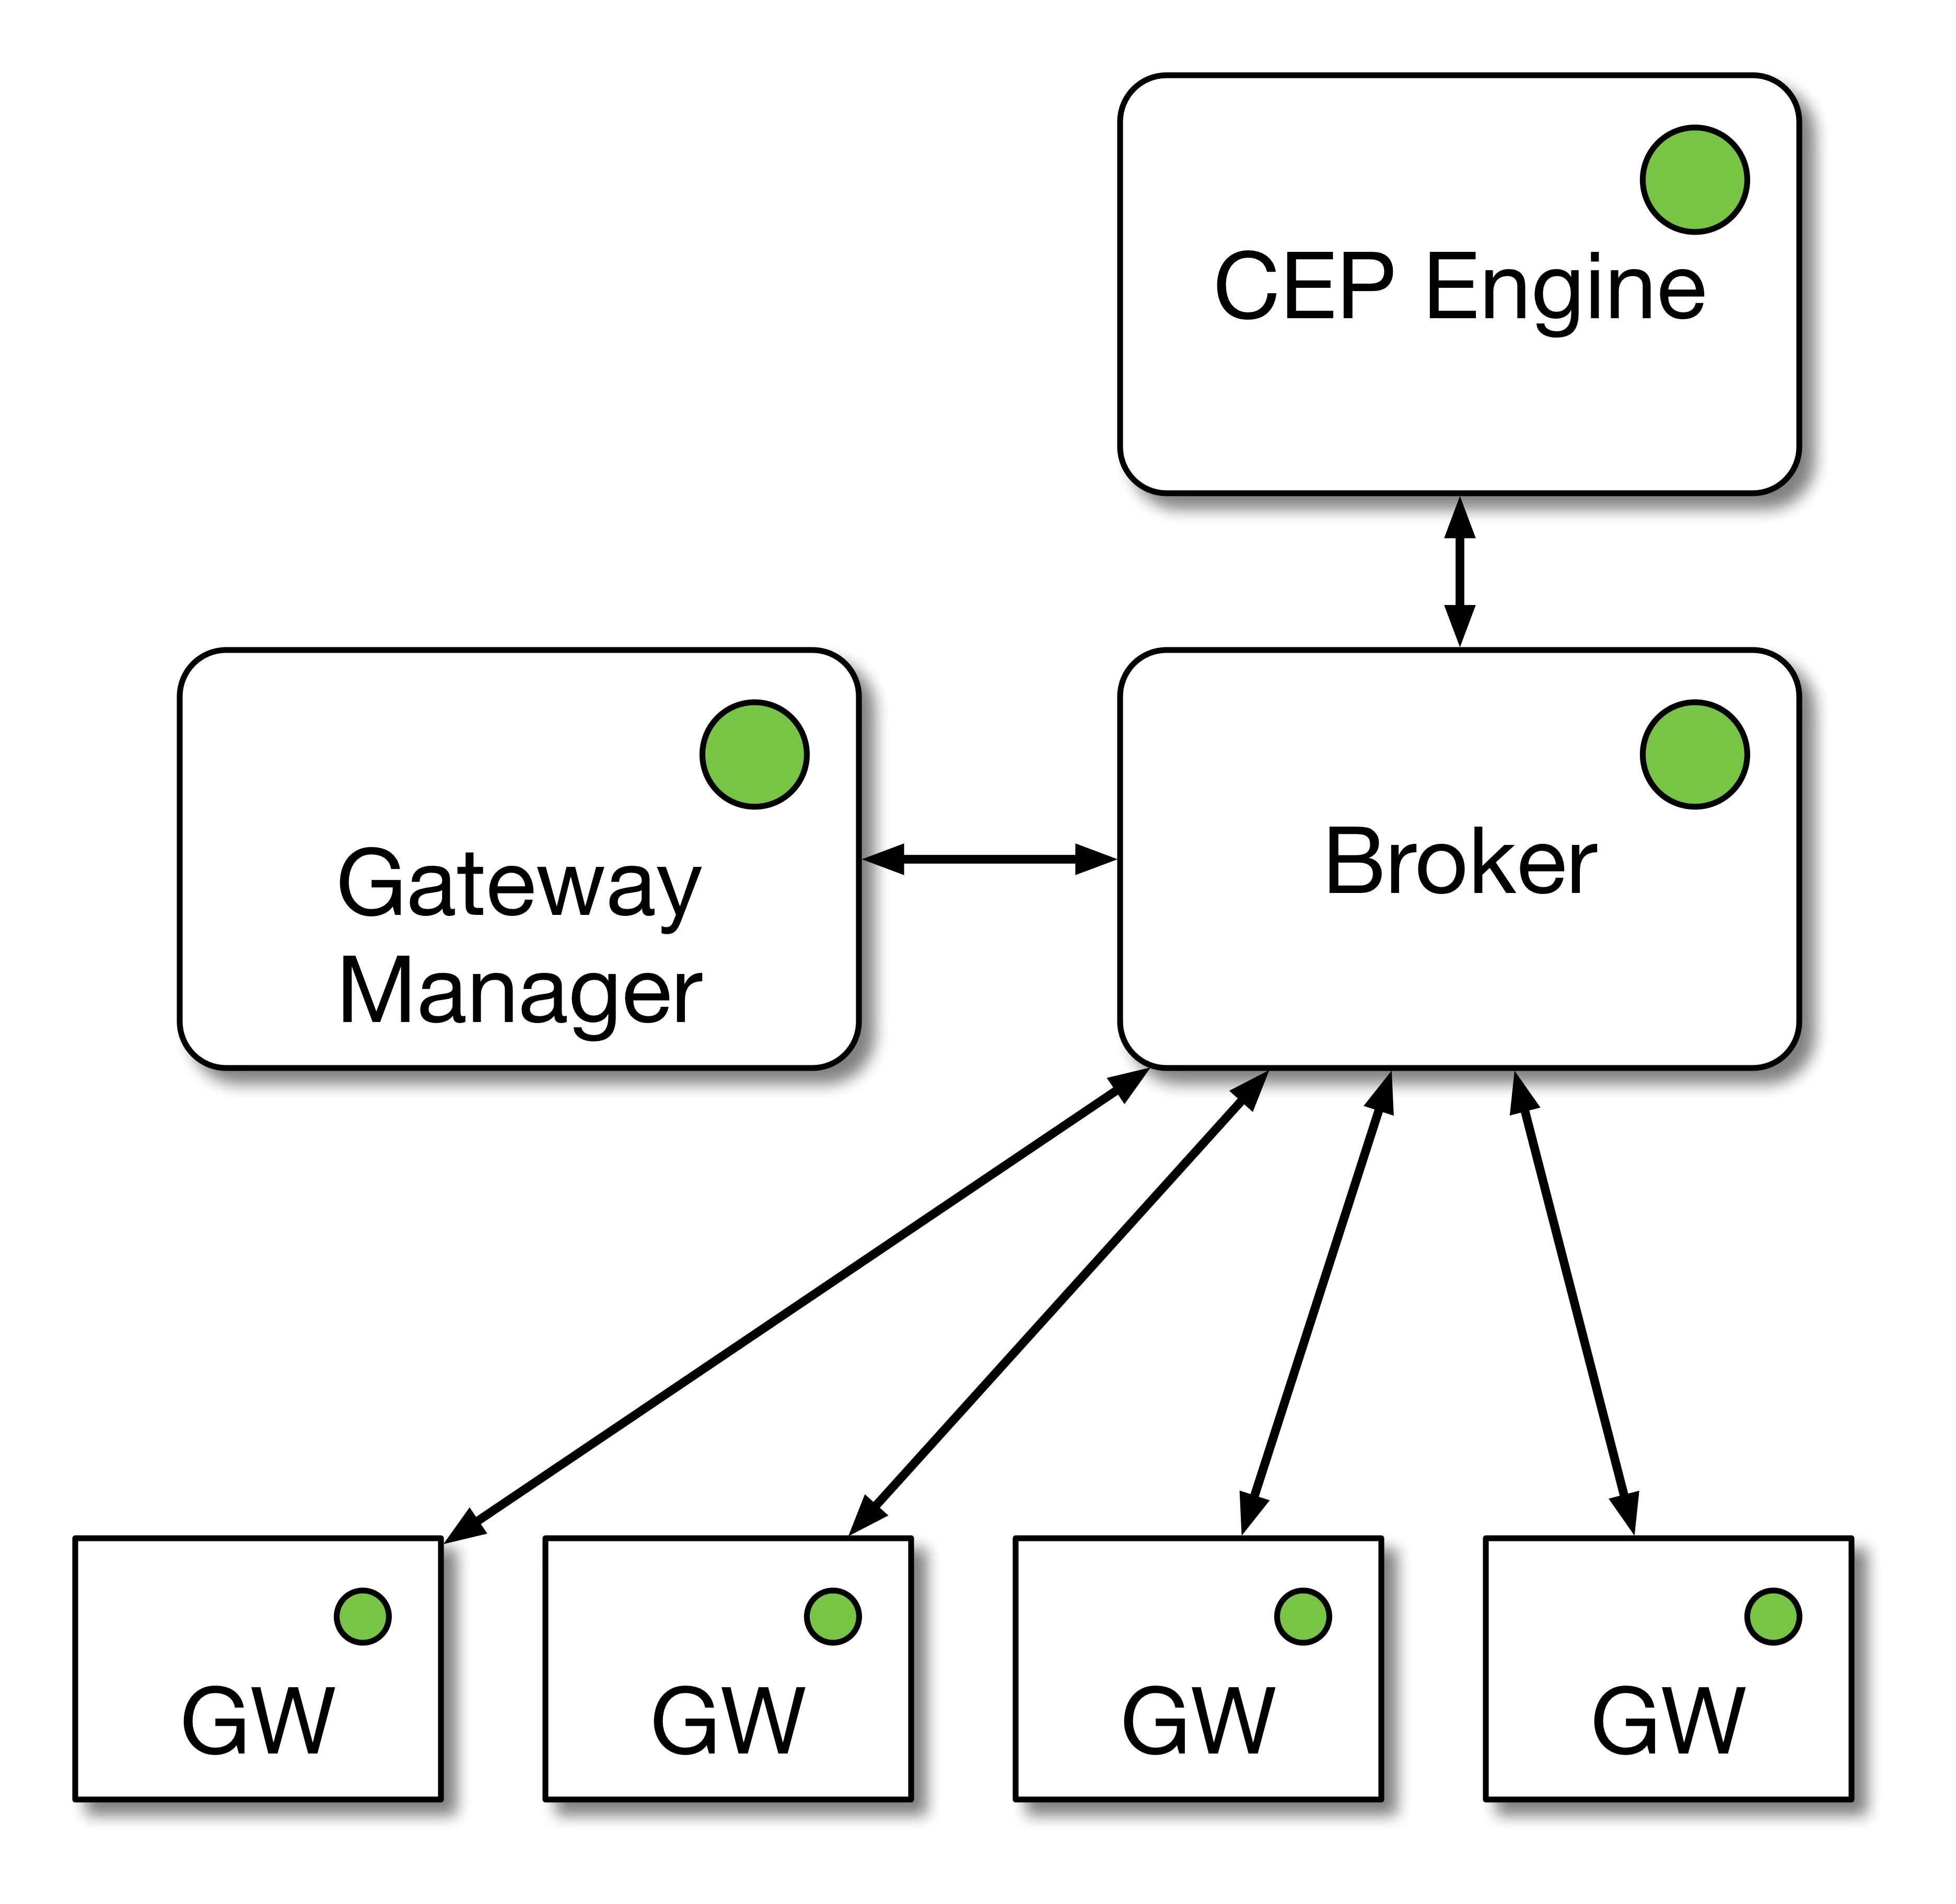
\includegraphics[width=0.4\textwidth]{figures/fs1.png}
		\caption{Simplified SmartLighting architecture.}
		\label{fig:sc1}
	\end{figure}
	
	This first scenario corresponds to the normal operation of the system, as shown in Figure \ref{fig:sc1}, where every component is working properly. In this case, the CEP module should receive events, generated by devices and sent to the message broker by gateways, process them and send the result to the message broker, and later to the corresponding gateway. 
	
	
	
\end{Paragraph}

\begin{Paragraph}{Scenario 2 - \ac{cep} Engine failure}
	
		\begin{figure}[H]
		\centering
		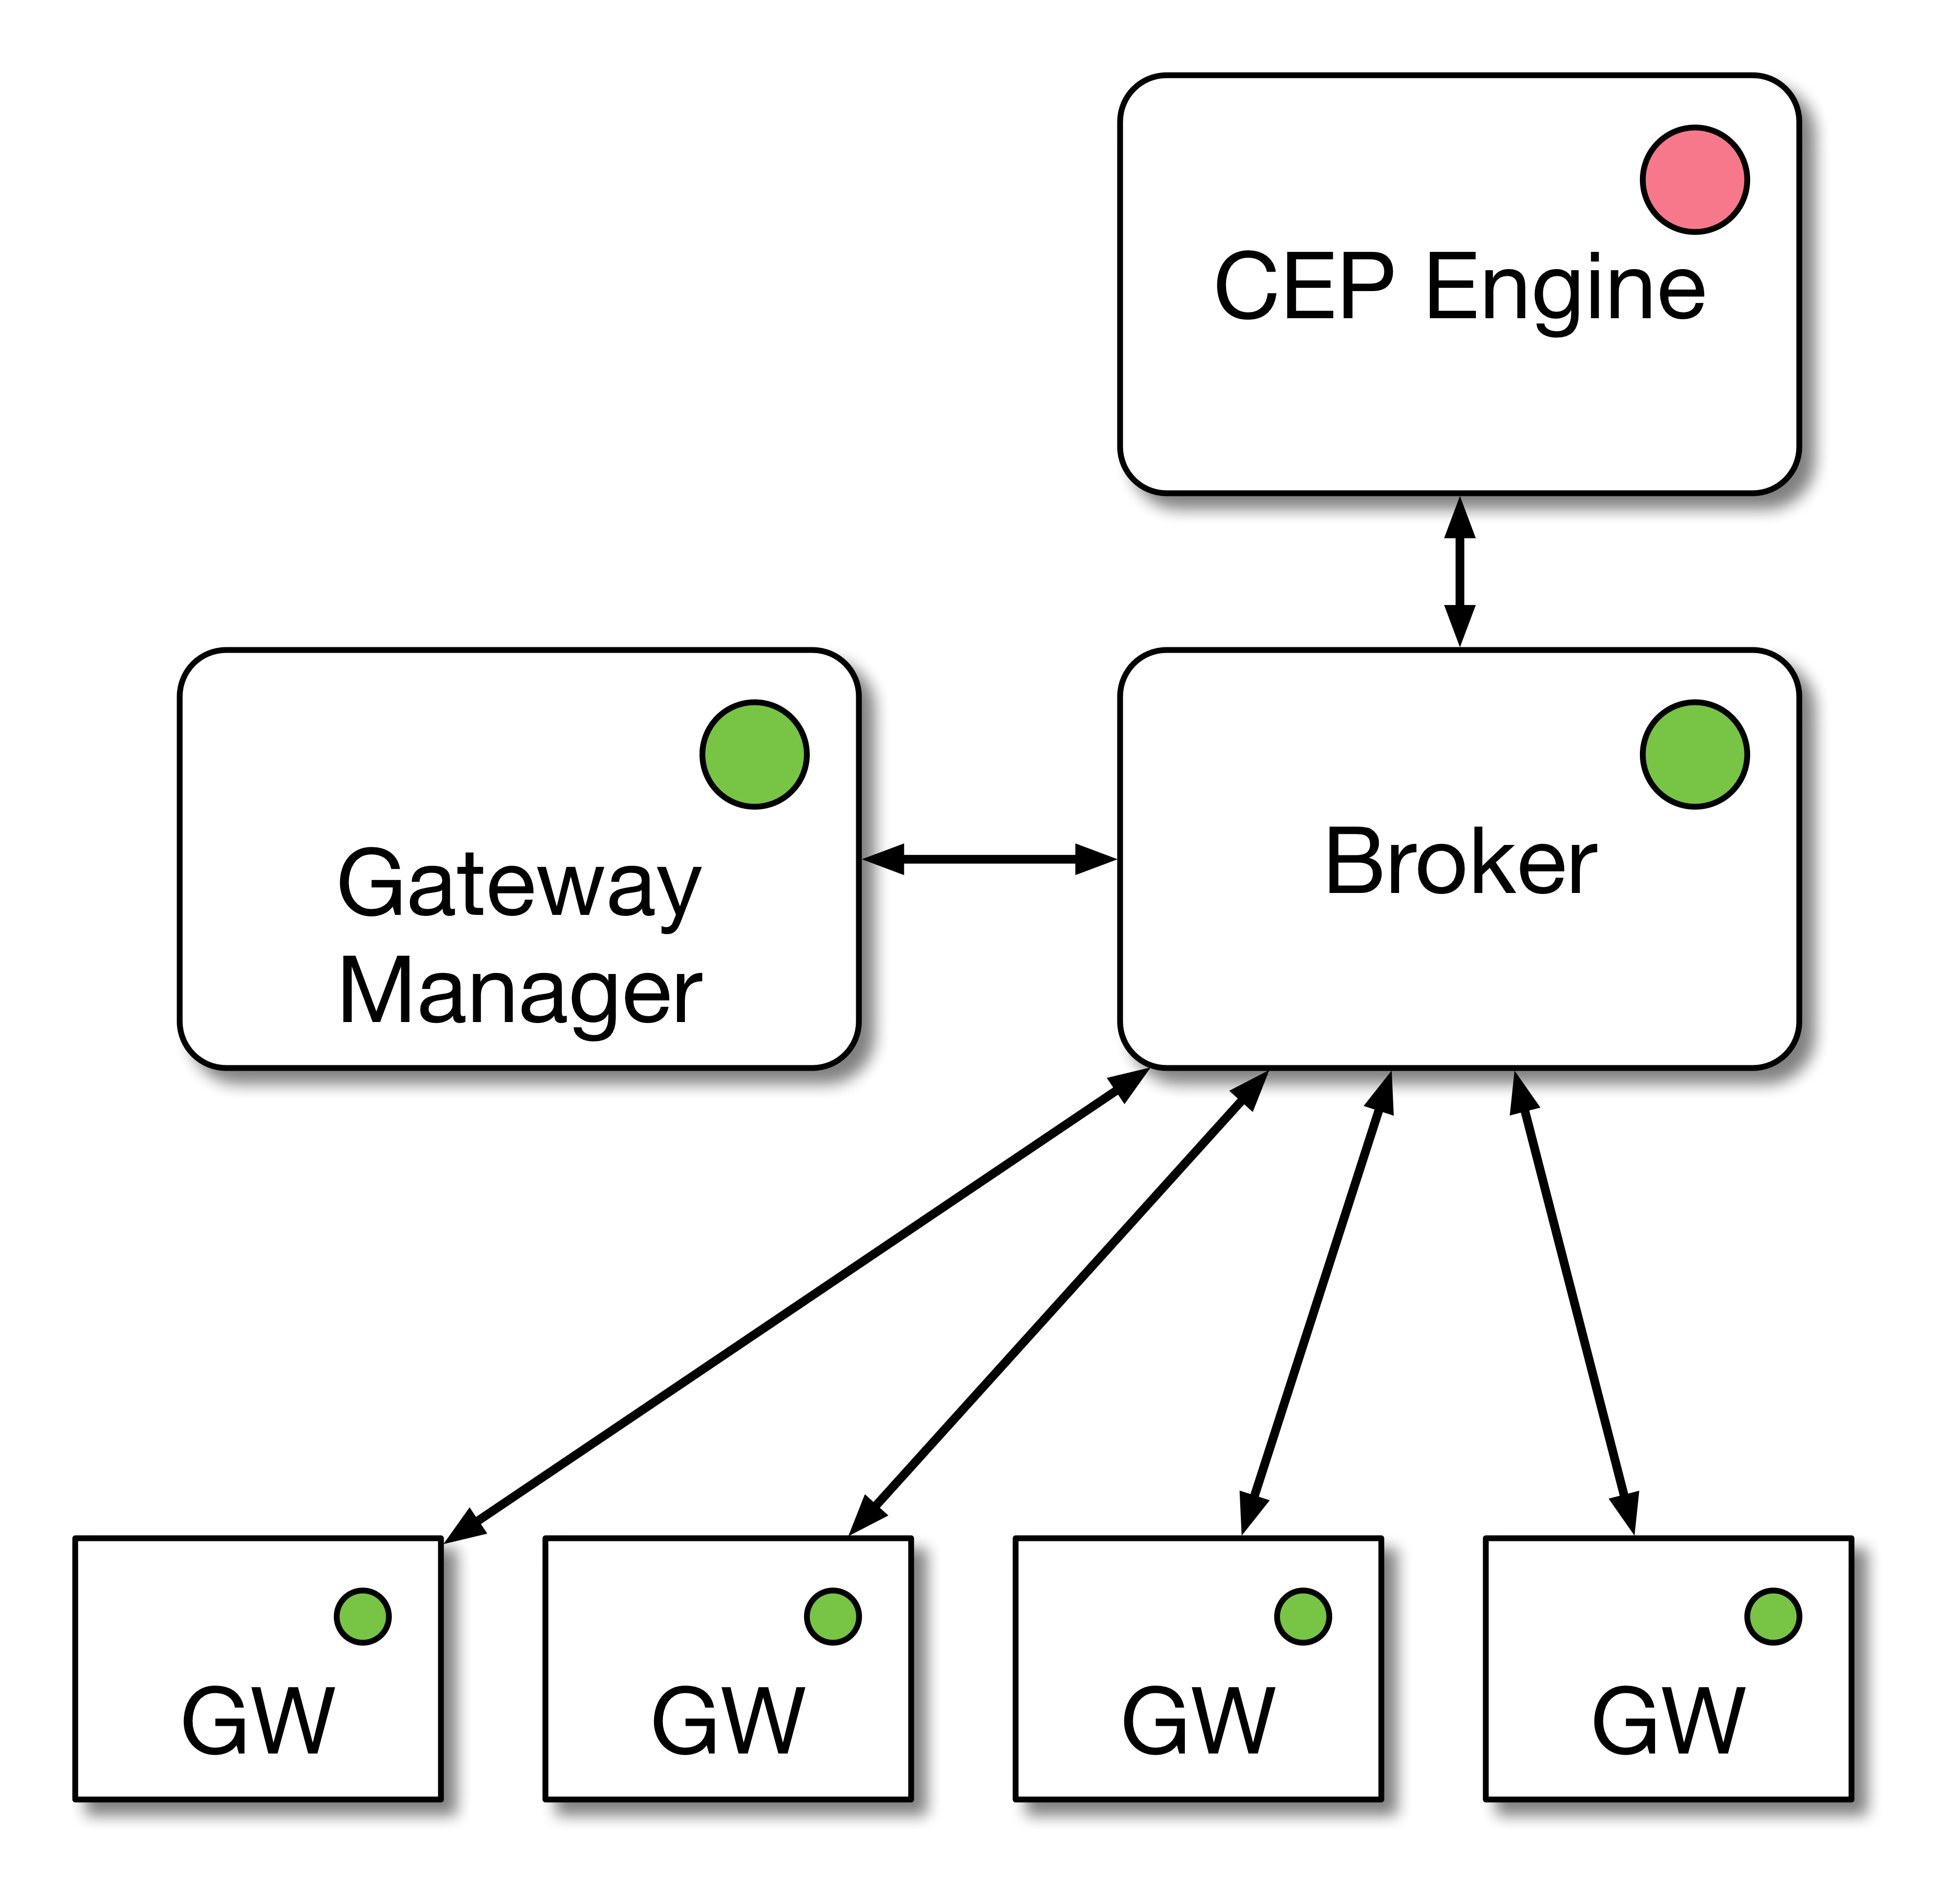
\includegraphics[width=0.4\textwidth]{figures/fs2.png}
		\caption{Functioning scenario 2.}
		\label{fig:sc2}
	\end{figure}
	
	In this second scenario, shown in Figure \ref{fig:sc2}, the CEP module fails and thus, the event processing is halted, either because the server where the program was running was down, or because of a failure in the connection between this component and the message broker. Either way, in this scenario, the generated events cannot reach the CEP Engine to be processed. Since one of the requirements for this project is granting that the building's basic functionalities, like lighting, still work, the system should be able to detect this failure and gateways should begin to process events. 
	
\end{Paragraph}

\begin{Paragraph}{Scenario 3 - Gateway Manager failure}
	
	\begin{figure}[H]
		\centering
		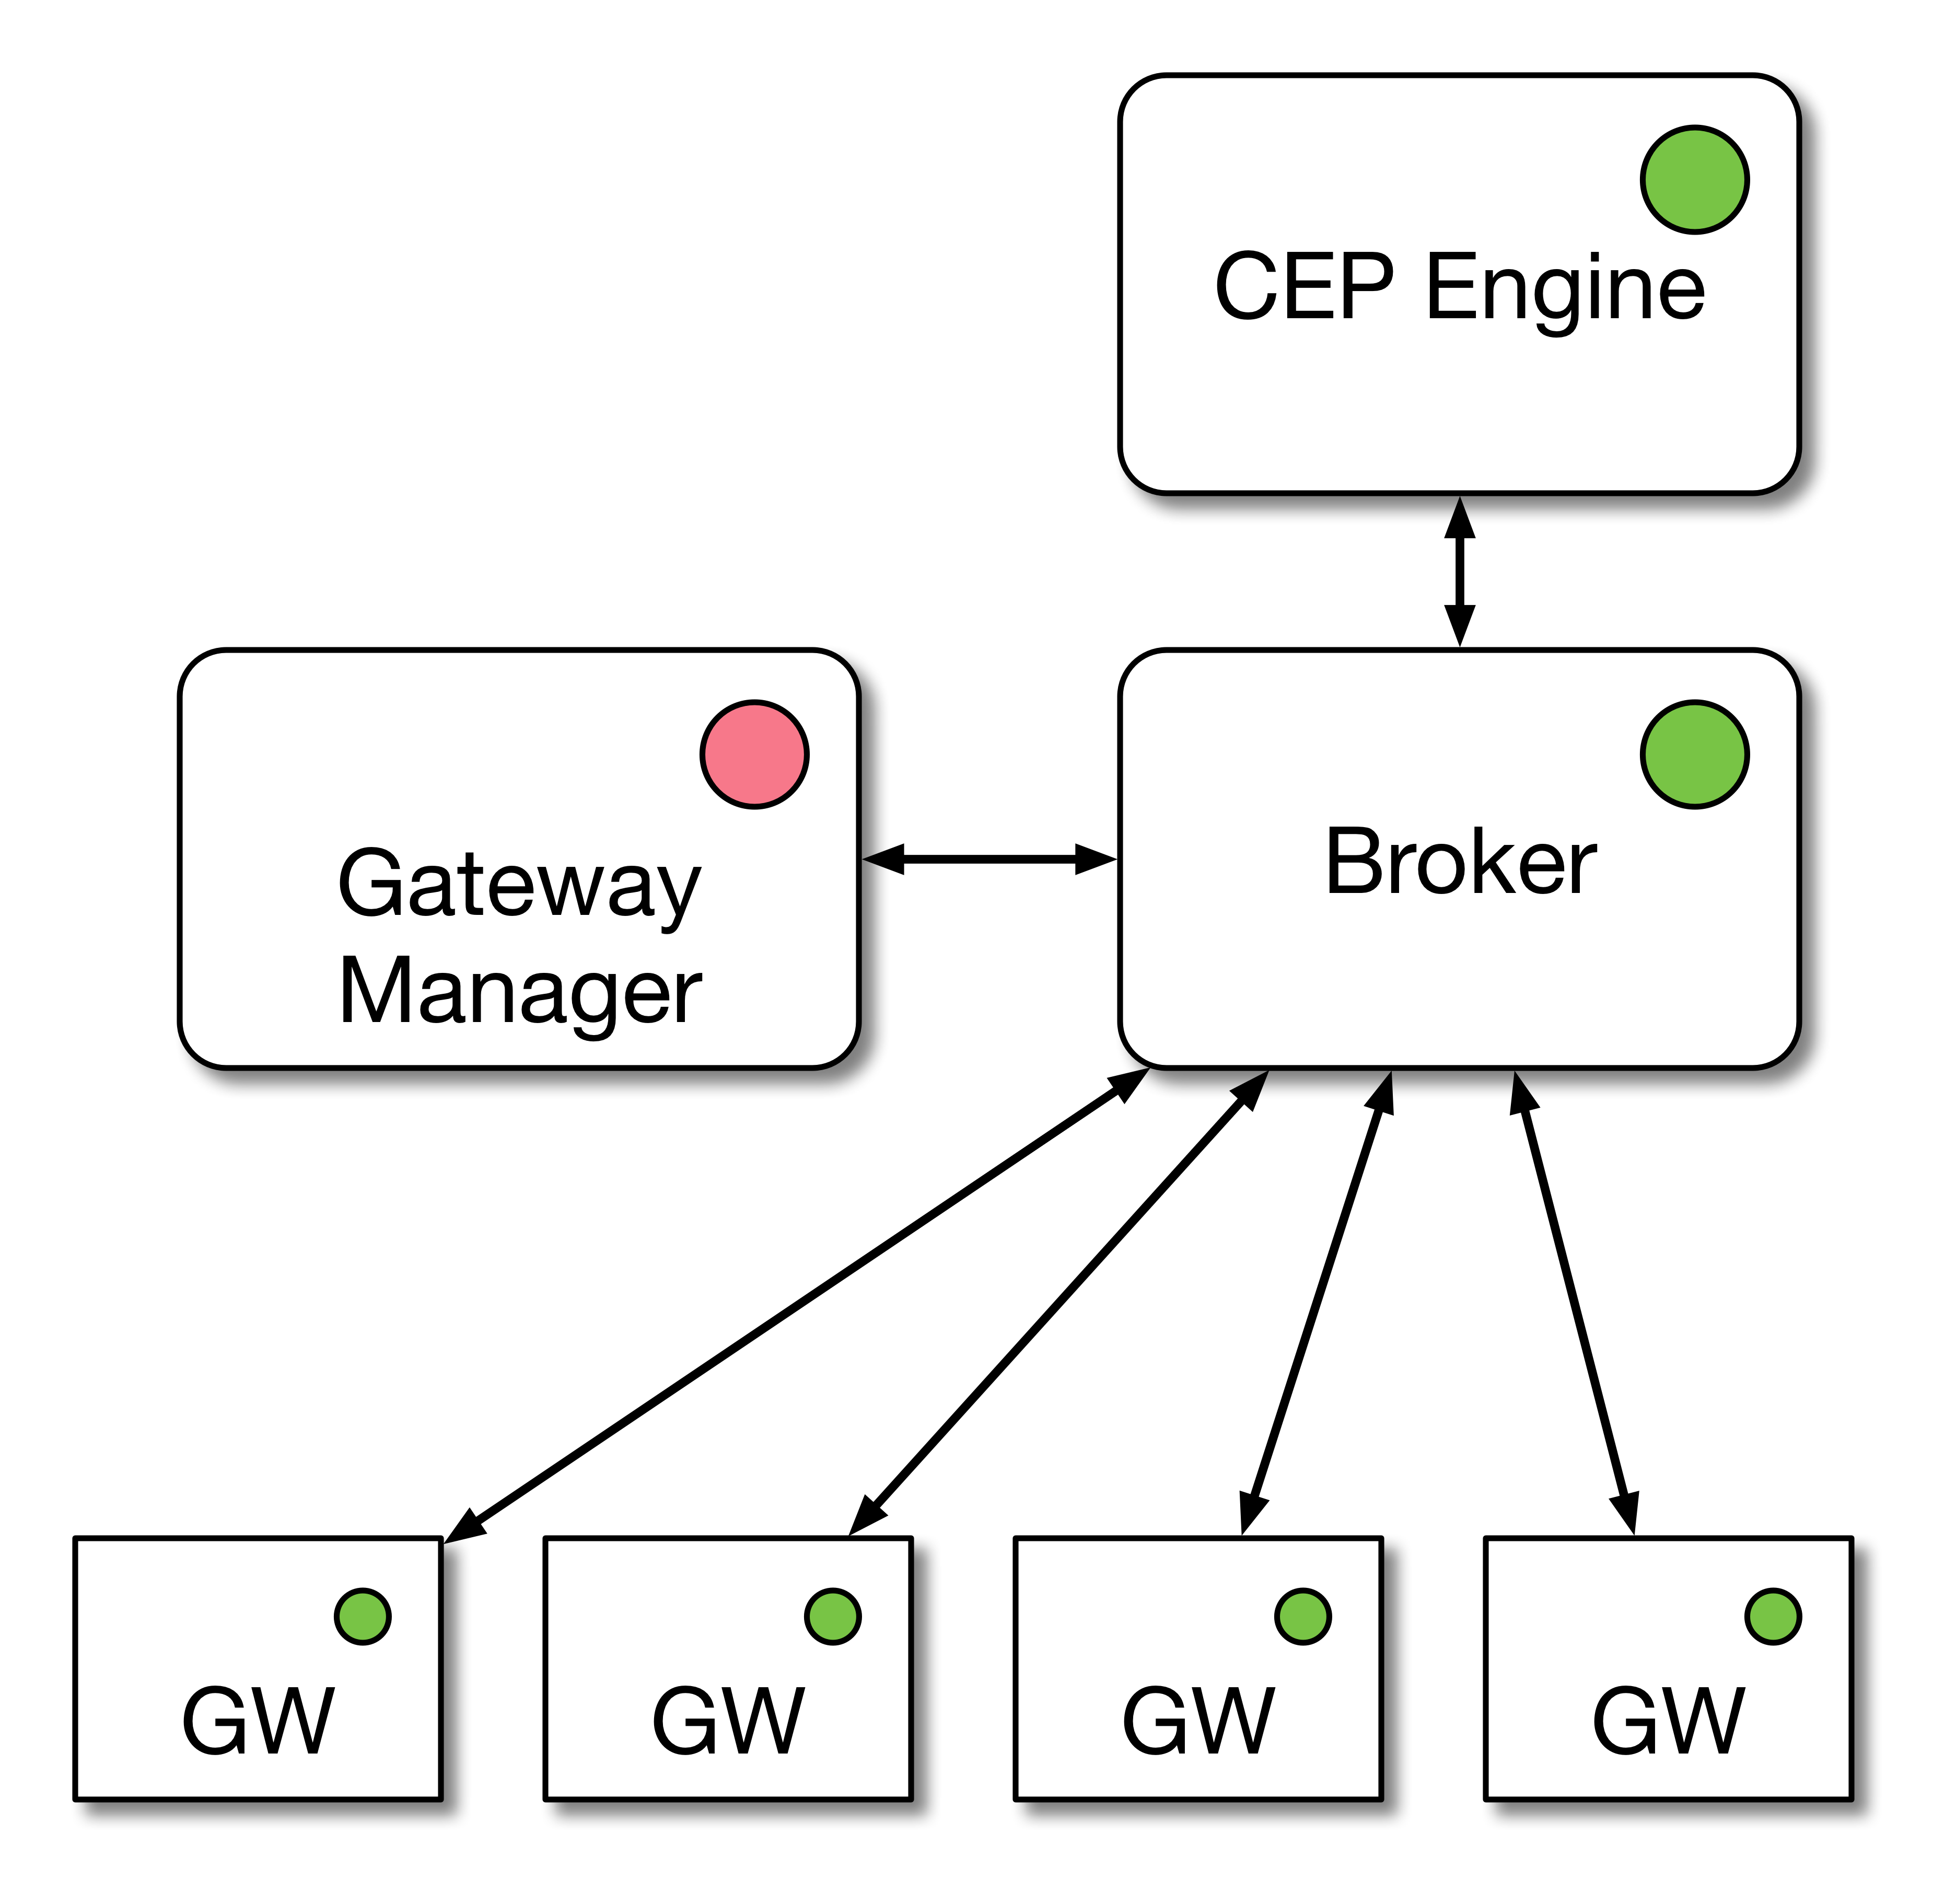
\includegraphics[width=0.4\textwidth]{figures/fs5.png}
		\caption{Functioning scenario 3.}
		\label{fig:sc3}
	\end{figure}
	
	Scenario 3 represents a failure in the Gateway Manager while all the other components are working correctly. Again, this failure can be due to a program error, a downtime in the server where the program is running, or because of a failure in the connection between this component and the message broker. When one of this situations happens, the system should continue to work correctly, however, since this component is responsible for distribute rules and devices through the accessible gateways, this features will not be available and thus, the automation of some building areas might stop working.
	
	
\end{Paragraph}

\begin{Paragraph}{Scenario 4 - Gateway Manager and \ac{cep} Engine failure}
	
	\begin{figure}[H]
		\centering
		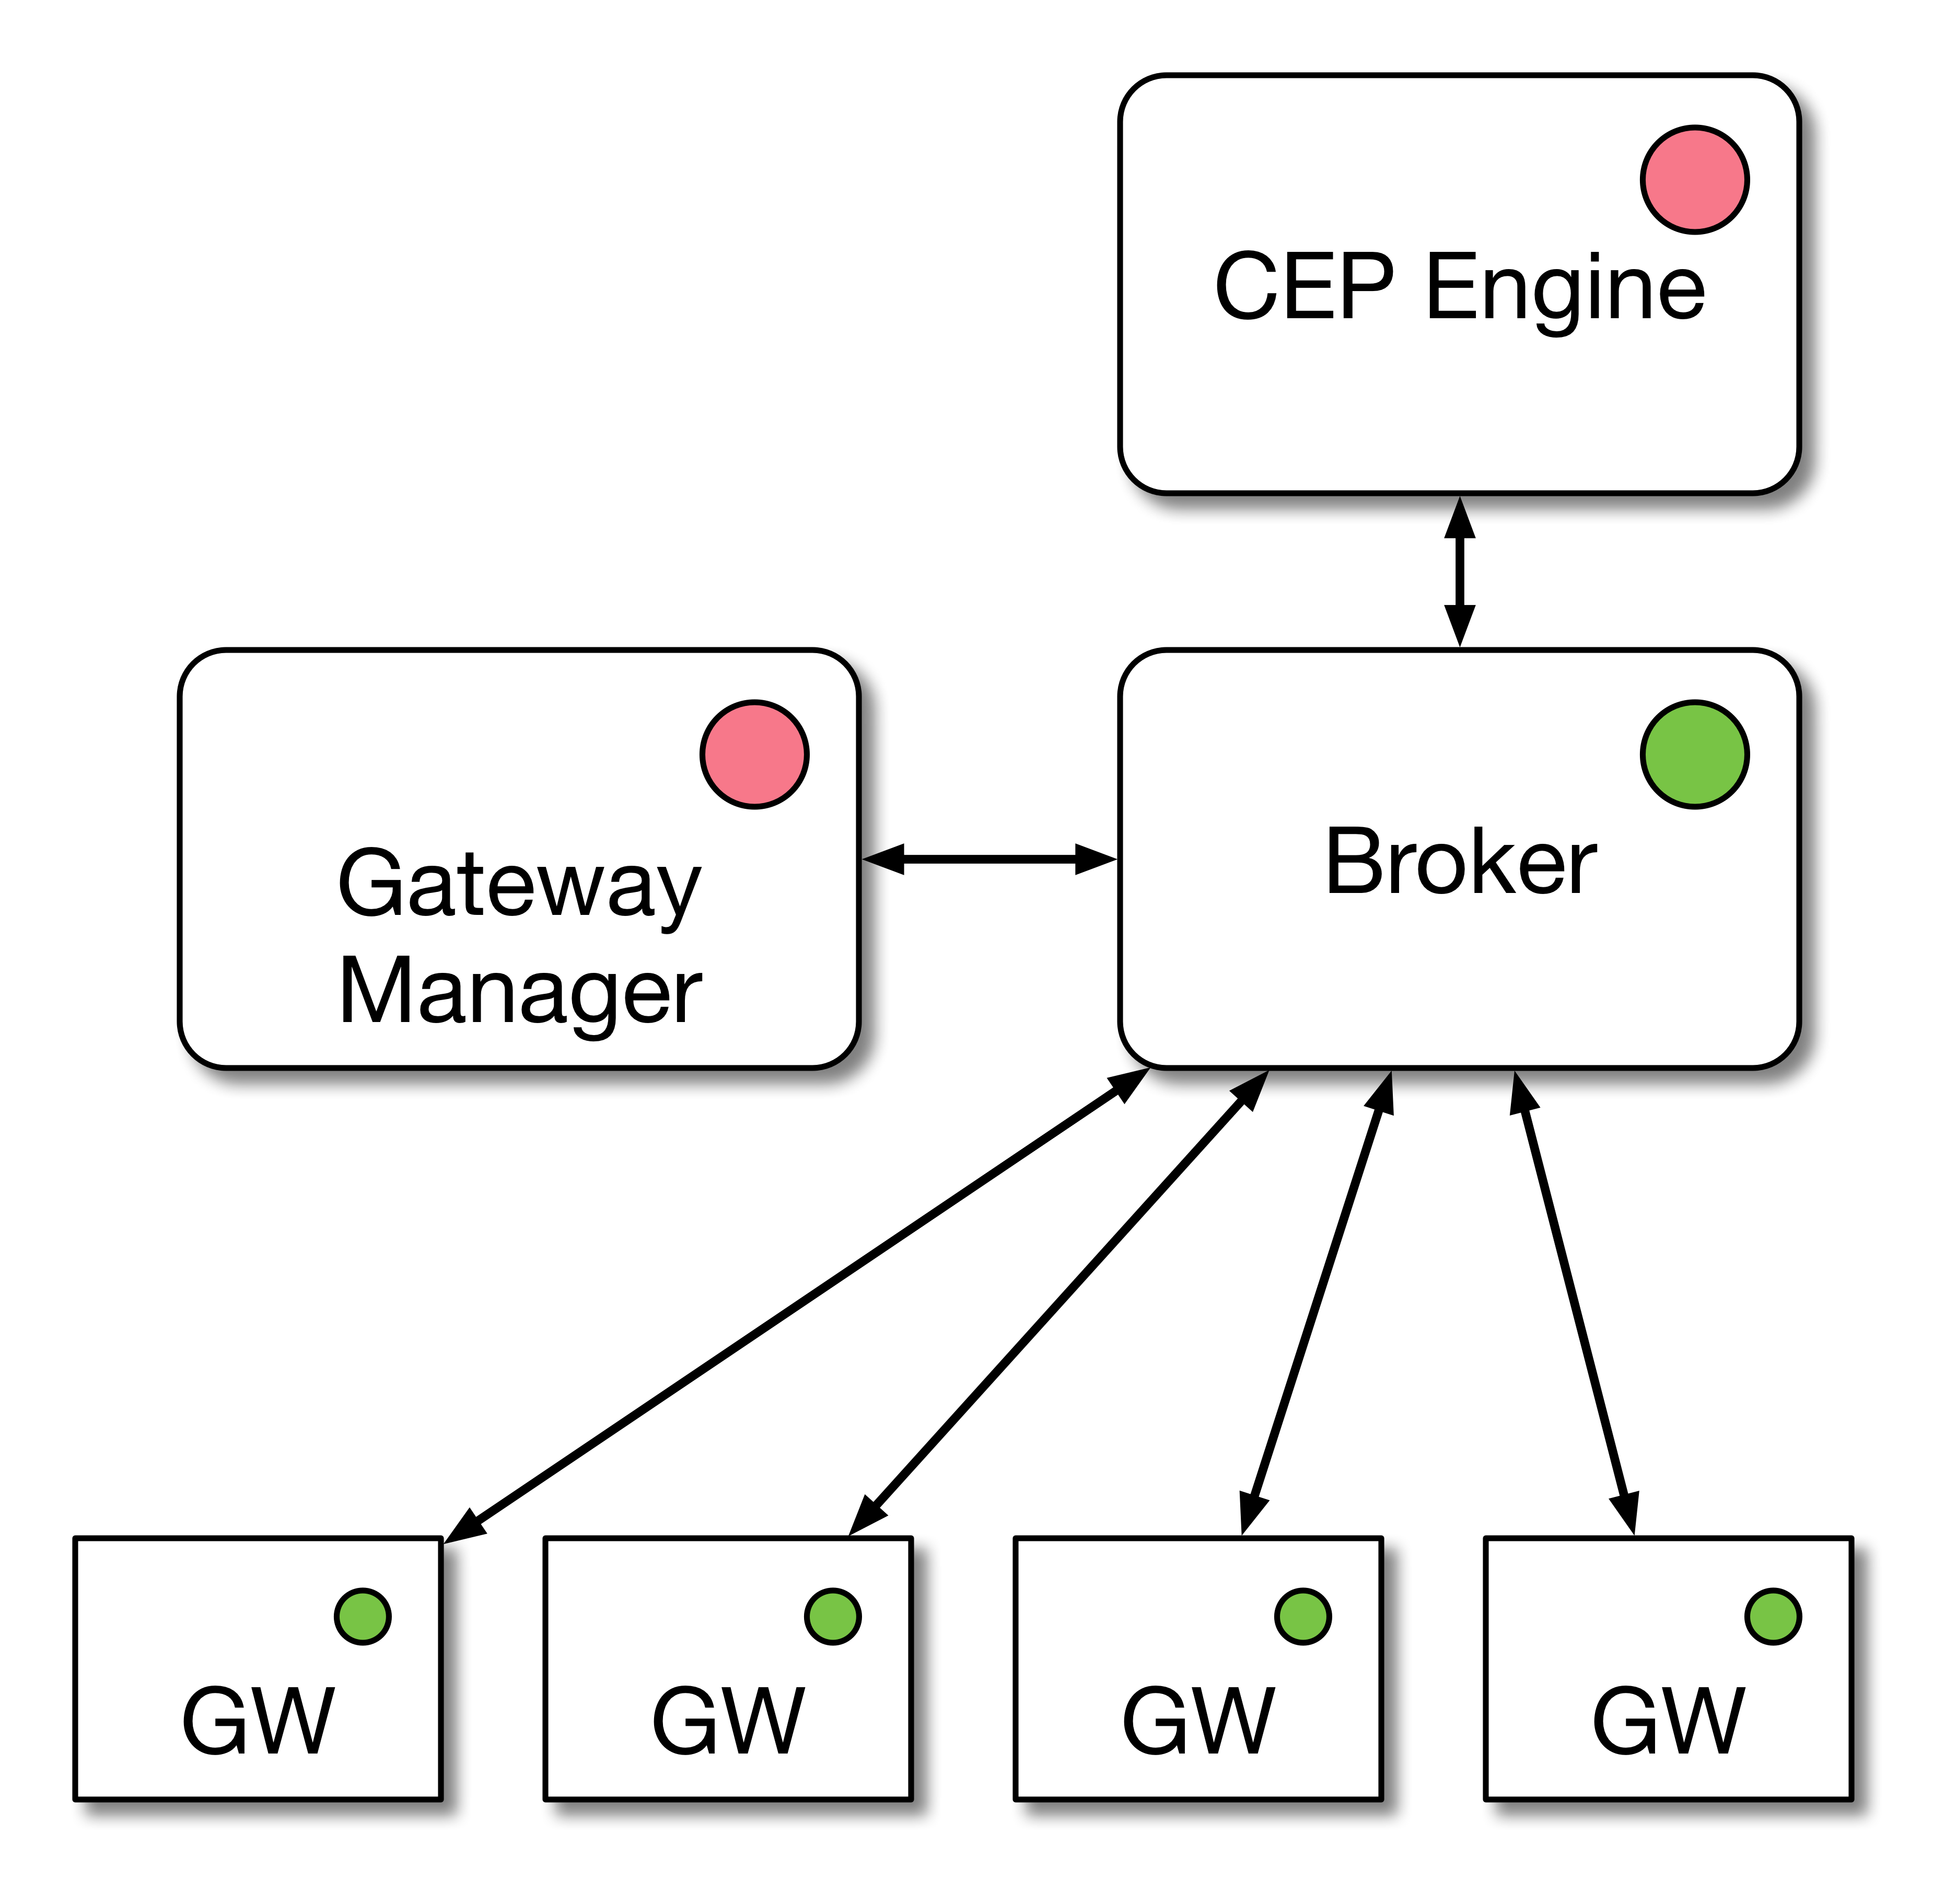
\includegraphics[width=0.4\textwidth]{figures/fs4.png}
		\caption{Functioning scenario 4.}
		\label{fig:sc4}
	\end{figure}
	
	This scenario corresponds to both the Gateway Manager and the \ac{cep} Engine being unavailable. This scenario is a combination of the failures shown in scenario 2 and 3, as both the CEP Engine and the Gateway Manager are no longer disposable. Again, this can happen if the two components fail internally at the same time, or the communication between them and the message broker is down. Based on what each component is responsible for, this scenario would made unavailable the processing of events in the CEP Engine and the rules and devices distribution to gateways performed by the Gateway Manager. In this scenario the system should continue the processing of events in the gateways, and make use, if necessary from the message broker.
	
\end{Paragraph}


\begin{Paragraph}{Scenario 5 - \ac{mqtt} Broker failure}
	
	\begin{figure}[H]
		\centering
		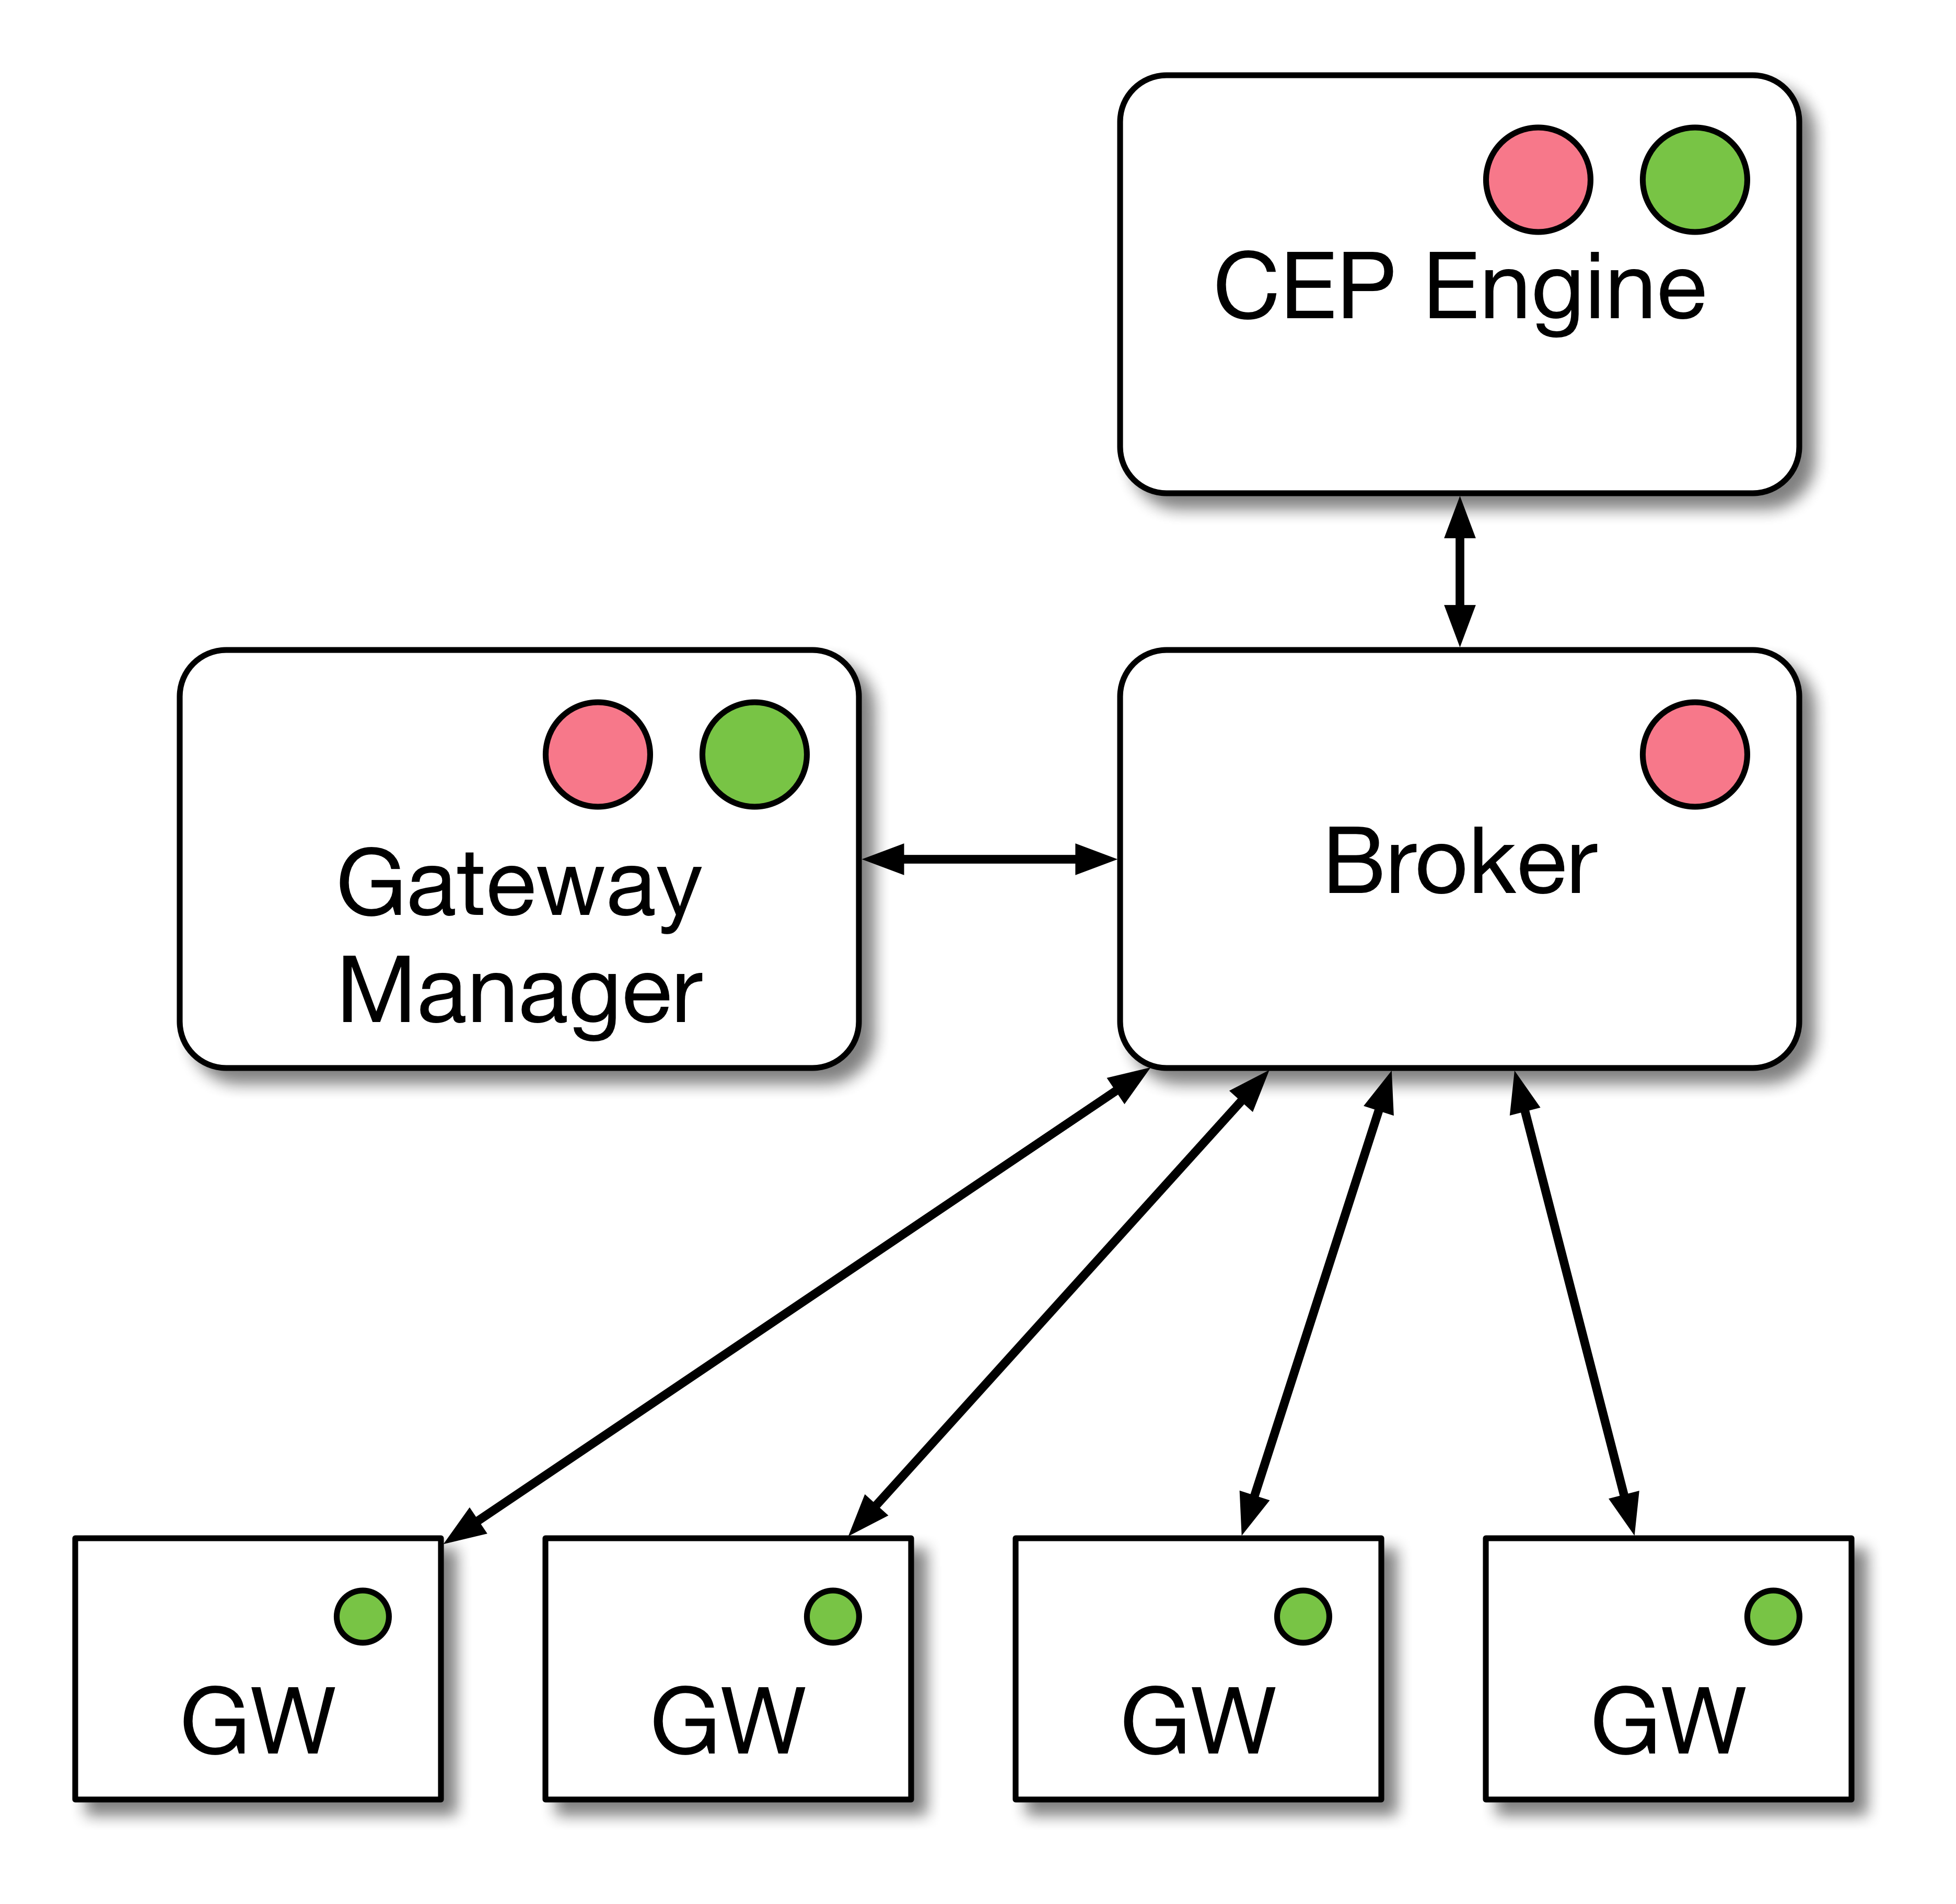
\includegraphics[width=0.4\textwidth]{figures/fs3.png}
		\caption{Functioning scenario 5.}
		\label{fig:sc5}
	\end{figure}
	
	The third scenario, shown in Figure \ref{fig:sc5}, when the message broker is down, the communication between gateways and the CEP Engine is cut off, so even if the CEP Engine and the Gateway Manager were still running, they would not be able to communicate with the gateways. This scenario can happen due to a network failure in the building. In this case, since every component, excepting the devices and gateways, are running in building servers, if the internal network was down, the gateways would be isolated and the devices would only be able to rely on the respective gateways, since the connection between the two would not be affected. This would be the most severe scenario, and the system should be able to grant the  minimum functionality by, for instance, process the device's events on the gateways, as said before.
	
\end{Paragraph}


In every scenario stated before there is a need for failure recovery of the gateways too. For instance, if a gateway gets disconnected, the other gateways should be able to take over the sensors and actuators previously owned by the failing gateway and act as a new gateway for them.








	\chapter{Implementation}
\label{chapter:implementation}

The objective for this chapter is to describe the steps and decisions taken, and the reasoning behind the implemented features. It starts in section \ref{implementation:objectives}, by presenting the objectives for the implementation, following by the used technologies on the several components in section \ref{implementation:technologies}. After that, in sections \ref{implementation:devices} and \ref{implementation:rules}, it is presented the standards used to access the devices and to define rules, respectively. Following, in section \ref{implementation:architecture}, the whole system's architecture as well as the functioning of its components is described. 

Since one of the requirements and objectives for this project was the existence of failure handling mechanisms, in section \ref{implementation:scenarios}, it is described the implementation taking into account the several scenarios addressed in the previous chapter. 

\newpage

\section{Objectives}
\label{implementation:objectives}

Although the implementation of the whole solution, presented in chapter \ref{chapter:architecture}, would be optimal to validate the project, it would be unrealistic due to the amount of time necessary to do so and the limited time available for this dissertation. Since some of the features were already implemented, such as a working platform to create and manage rules, a \ac{cep} engine and a simple gateway to communicate with devices through BLE, this dissertation's main focus was in the implementation of gateways capable of implement automation rules, alike to the ones implemented by the CEP engine, as well as give them means to adapt to failing and emergency states. For that reason, was also implemented a gateway manager to act as a monitor for the gateways, being able to control not only the functioning of each one of them as well as manage the distribution of rules and devices throughout the gateways.

Looking at the architecture presented in chapter 3, the component for the user management dashboard was not implemented for the scope of this work. Apart from this, all the features mentioned were implemented and are detailed in the continuation of this chapter.



\section{Adopted  Technologies}
\label{implementation:technologies}

This section aims to discuss the technologies chosen for the different components of the architecture. These choices will be justified and explained taking into account the requirements for this project, however, it is important to note that there are no perfect solutions and, in some cases, several approaches could have been taken. 

Since there was a dissertation\cite{helder} that already implemented some features like the \ac{cep} engine and the \ac{bm}, some of the technologies used in this dissertation were influenced by past decisions. As far as the \ac{cep} engine concerns, the choice was the WSO2 \ac{cep} \cite{wso2}, since its features addressed all requirements, that such system would need, to fit this project's requirements. For the purpose of this dissertation both the \ac{cep} engine and the \ac{bm} as well as the communication between them, did not affect any of the new implemented features, however, since MQTT protocol was primarily used as the elect protocol for communications in the referred dissertation, the implemented features presented in this work followed the same path.

Finally, it is important to state that the standard used, in SmartLighting project, for both object definition to read and write information to/from devices, and the rules structure, were also maintained and will be described in the following sections. 

\section{Access to Devices}
\label{implementation:devices}

Devices like sensors, which measure environment changes, and actuators, and may trigger mechanisms to make changes in that same environment, are fundamental pieces to implement a smart and automated environment. Since there are a huge variety of devices with different characteristics, in order to enable extensibility for the system, the access to those devices, as well as the messages format, should be standardised. In another dissertation for this project, a standard following the IP Smart Objects Alliance Guideline\cite{IPSOAlliance2014} was made and is illustrated in Figure \ref{fig:obj}

\begin{figure}[H]
	\centering
	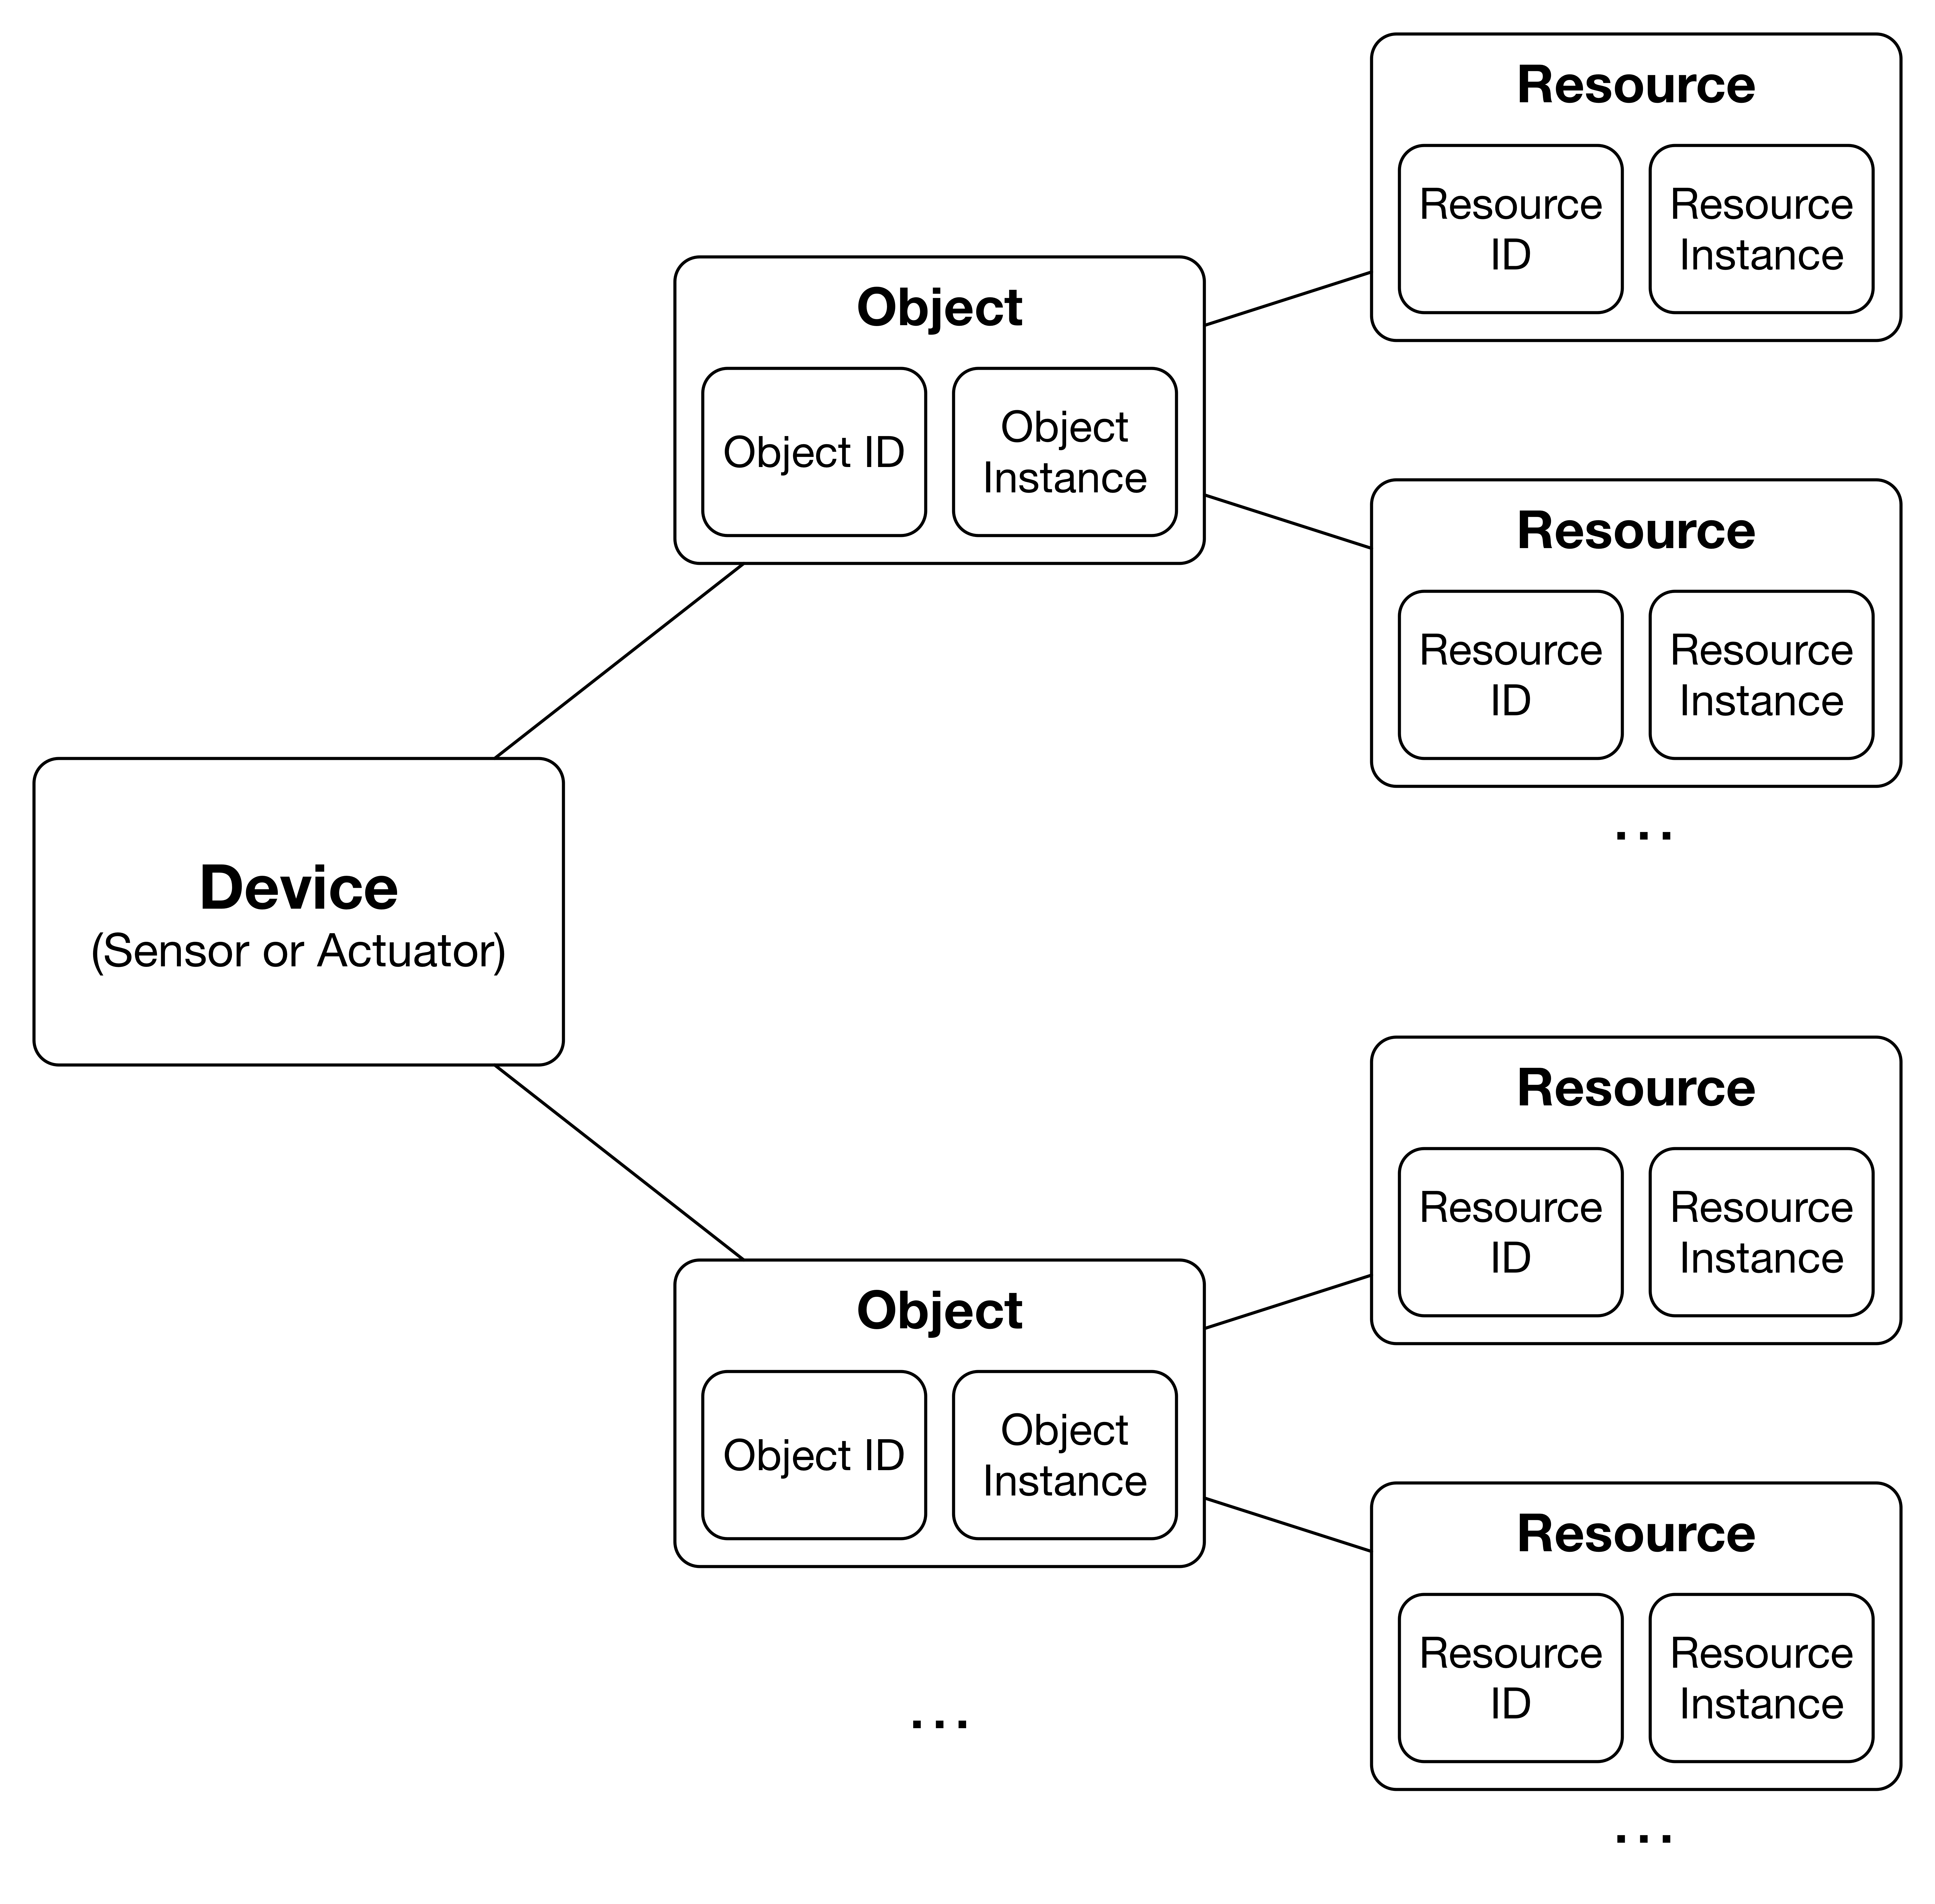
\includegraphics[width=0.9\textwidth]{figures/obj.png}
	\caption{Device objects representation}
	\label{fig:obj}
\end{figure}

In this representation, a device can have multiple objects (sensors and/or actuators), identified through an ID and an object instance. As example, a device can have multiple sensing or actuating capabilities, each one of them identified with a different ID. A device with two motion sensors, will have two objects with the same ID but different object instances. 

Inside the representation of each object, the information is divided in resources. Resources represent the available features that each object provides, such as the available values that can be read or written, or the actions that can be triggered. As an example, an luminaire actuator object can have resources to read the current state of the luminaire, turn  on/off or dim the light to a certain value, each one of them represented with a different ID. The resource instance is used when, per example, when an actuator for aluminaire with two lamps offers the same resources for each lamp separately.

Using this representation, the properties of a device can me accessed using an Uniform Resource Identifier (URI) the following way: 


\begin{minted}[
frame=single
]{nginx}

.../Object_ID/Object_Instance/Resource_ID/Resource_Instance
	

\end{minted}
	
For instance, a device with a temperature sensor that offers the possibility of check the current state or check the minimum value measured by the sensor since it is ON, can be illustrated and accessed the following way:


\begin{figure}[H]
	\centering
	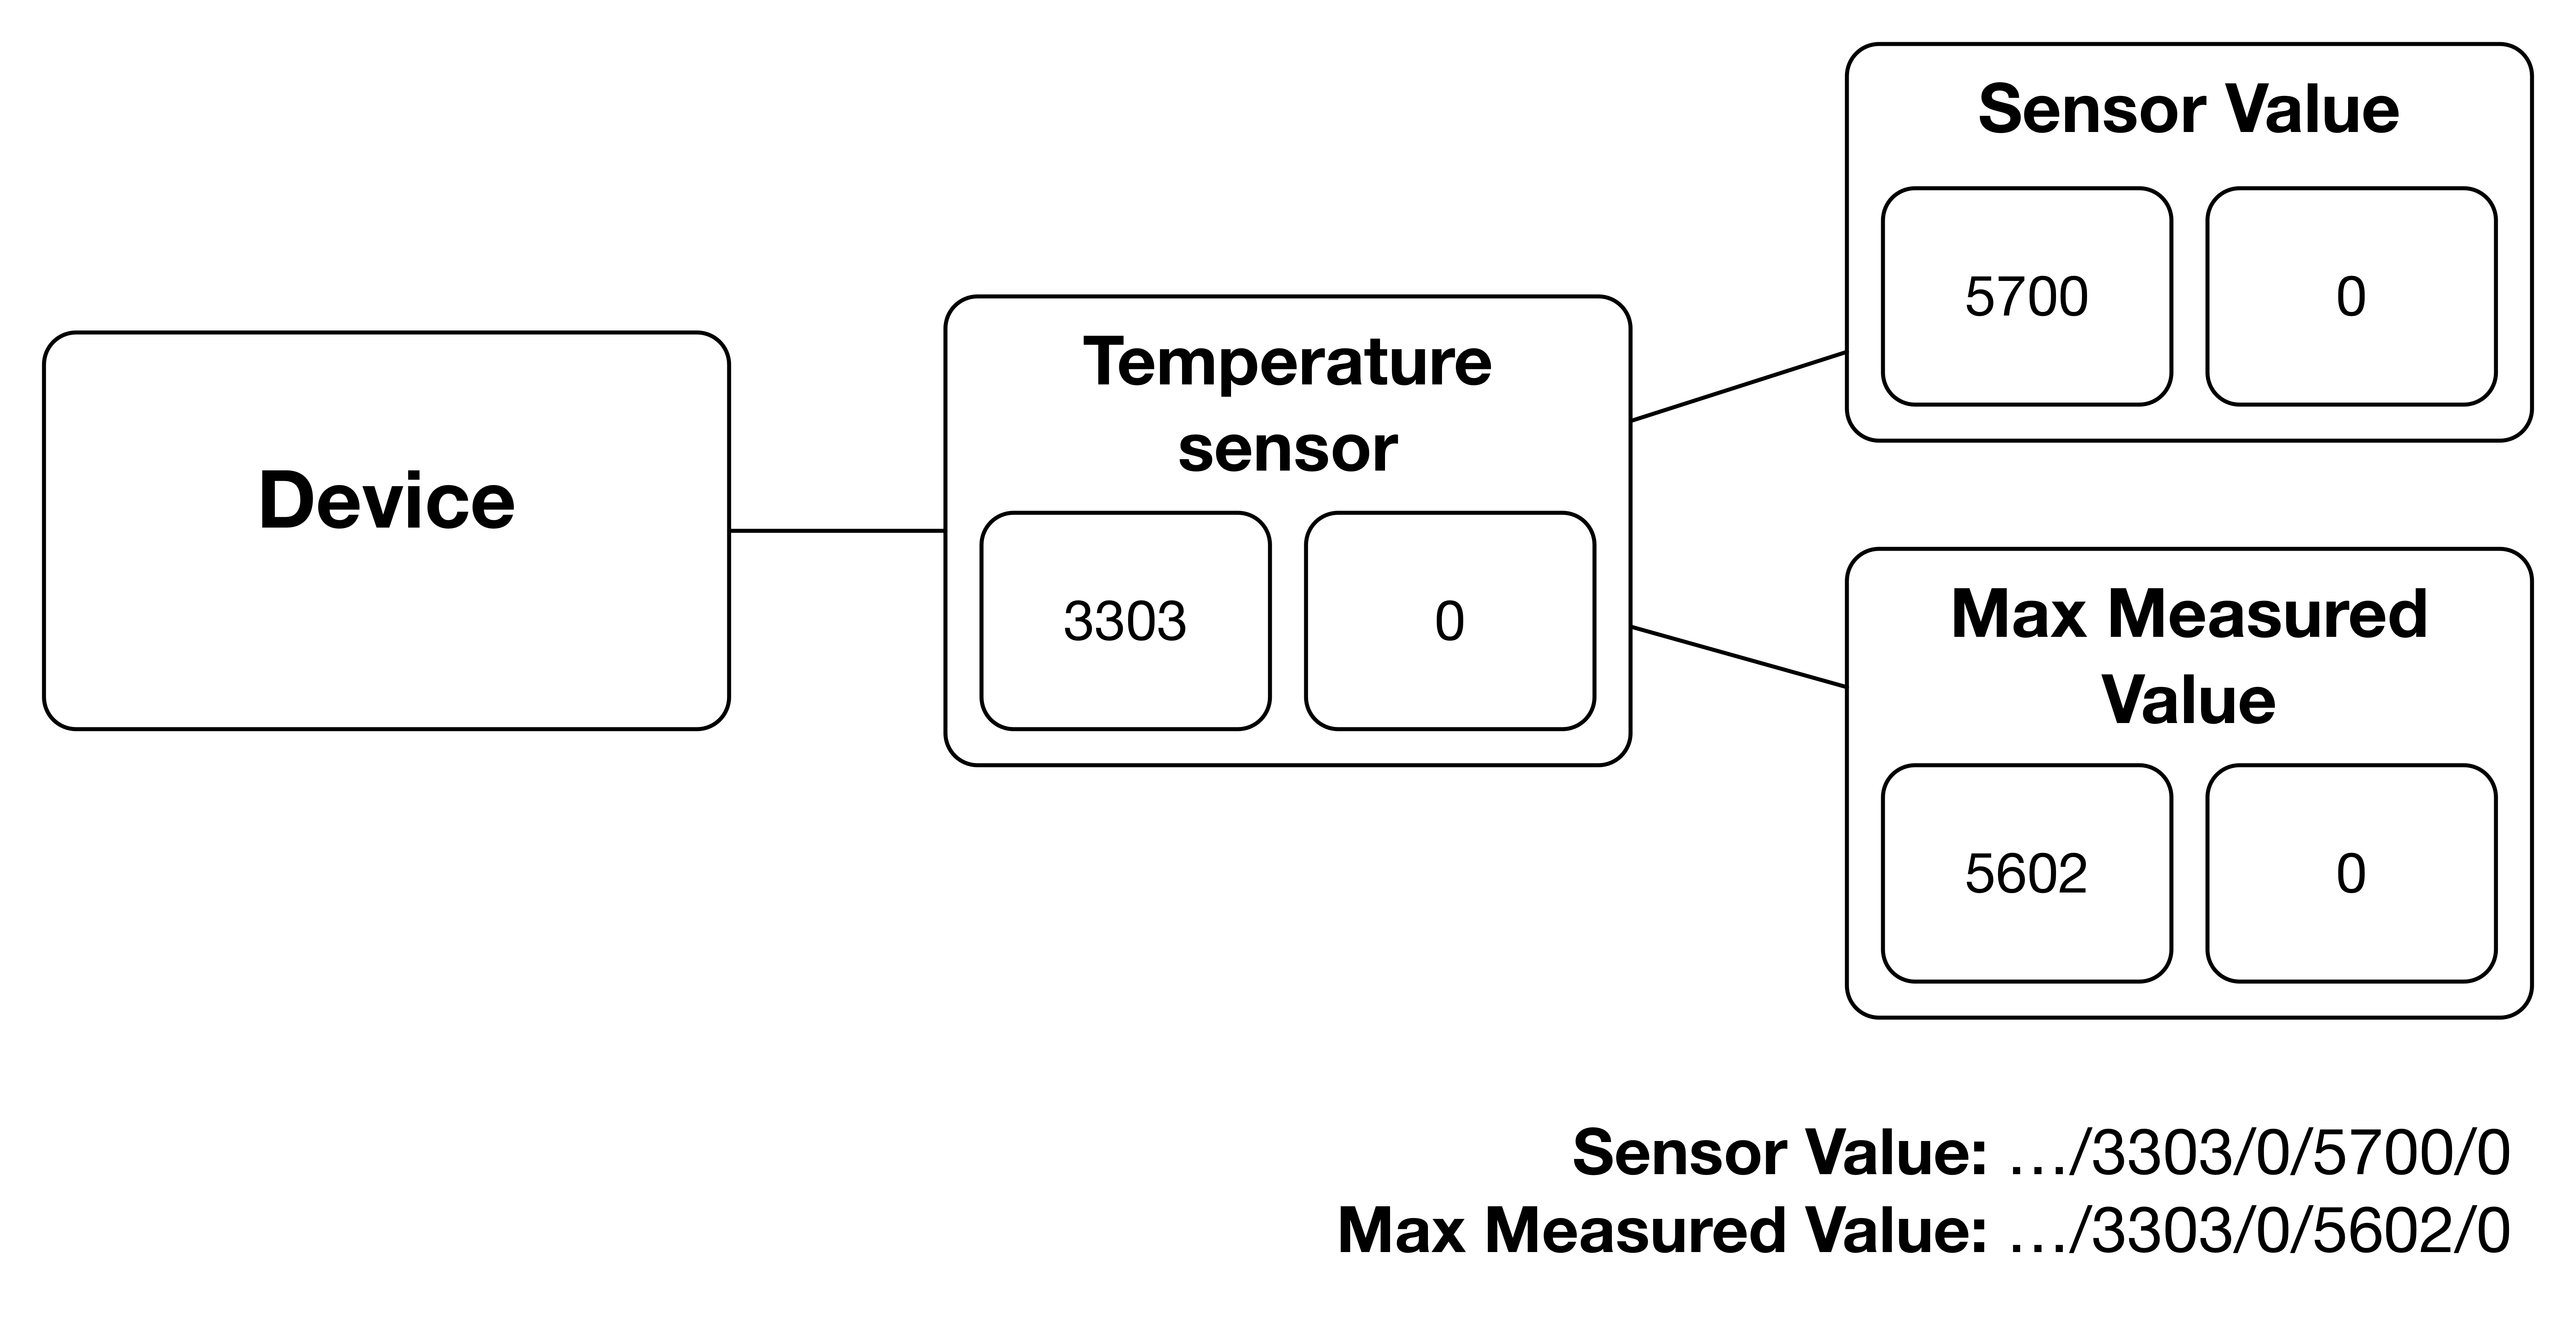
\includegraphics[width=0.9\textwidth]{figures/obj2.png}
	\caption{Access to a device resources.}
	\label{fig:obj2}
\end{figure}
	
Since the protocol used for this project was \ac{mqtt}, which allows to subscribe and publish messages in specific topics, this URI can be used in the topic to address each device resource. 


Since the WSO2 \ac{cep} was chosen as the complex event processor for this project\cite{helder}, a message format to communicate with devices, supported by that engine, was chosen.The format is represented in Snippet \ref{snippet:example}.

\begin{listing}[H]
\begin{minted}[
frame=single
]{json}

{
    "event": {
        "metaData": { 
            "attribute_1": ***,
            "attribute_2": ***,
            ...
        },
        "correlationData": {
            "attribute_1": ***,
            "attribute_2": ***,
            ...
        }, 
        "payloadData": {
            "attribute_1": ***, 
            "attribute_2": ***,
        }
    }
}


\end{minted}
\caption{Example of a simplified message for an event sent to a device.}
\label{snippet:example}
\end{listing}

These event messages are divided in three main logical sections: Payload Data, Correlation Data and Meta Data. Payload Data is the most important data to be transported, such as, the values that are sent to and from devices. The Correlation Data transports information that allows correlating events and lastly, the Meta Data is where other attributes that describe the event can be included. In Snippet \ref{snippet:todevice} is represented an example message of an event sent to a device.

\begin{listing}[H]
\begin{minted}[
frame=single
]{json}
{
    "event": {
        "metaData": {
            "operation":"set"
        }, 
        "payloadData": {
            "value": 15 
        }
    } 
}

\end{minted}
\caption{Example of a simplified message for an event sent to a device.}
\label{snippet:todevice}
\end{listing}

This message would set the value 15 on a device's resource if sent to the corresponding topic using the format presented above.

\section{Rules Standard}
\label{implementation:rules}


To obtain a fully autonomous system, rules must be designed in order to achieve it. In a former work for SmartLighting project\cite{helder}, a solution was designed to, instead of using directly the languages provided by each \ac{cep} engine which are difficult to map using a Graphical User Interface, a more extensible and pluggable solution was created. When a rule is made in the platform, a JSON is generated containing all the information needed to convert the rule to the desired engine, either the \ac{cep} engine or the Gateway engine, that will be addressed later.

In this solution, a Rule is divided in Actions, each one containing a Target and a Function. The Target specifies to where the output events, resulting from applying the rule, should be sent, while the Listeners inside the Function specify which input events trigger the rule. Also inside the Function, there can be present four types of modules to transform the event stream: Aggregators, Converters, Windows and Filters. Filters are used to select only events that pass a certain condition, otherwise the rule is not applied. Windows, allow to capture events in a given interval of time or occurrences following some criteria. This module is often used with Aggregators that perform aggregate calculations, such as summing the events or calculating averages. Lastly, the function of Converters is to make calculations with each event, for instance to preform unit conversions. There can also be used the Pattern and Sequence modules that, as the name says, are used to detect patterns or specific sequences of events.


In Snippet \ref{snip:rule} in Appendix A, is shown an example on an output JSON of a rule with a single action. As can be observed, a rule can be constituted by sub rules. Each sub rule within a Rule has the same Function but different Targets and Listeners. In this particular case, the rule has a function called "setif\_value\_percent" with two different types of Listeners, a "listen\_boolean" and a "listen\_value". The first is used to listen to boolean values (which in this case are the motion sensor state) and the last to listen to float values (luminance sensors, in this case). The boolean data is read for a 6 seconds time window and aggregated with the “any” Aggregator which detects if there was any motion in the last 6 seconds. The data containing the luminance values, is aggregated with an average over the last 5 events, and converted using the converter “lux\_to\_percent”. Therefore, the function sends to the target an event with the 100\% calculated percentage if a motion is detected in the last 6 seconds, and 50\% otherwise. 





	
\section{Architecture}
\label{implementation:architecture}
Taking into consideration the objectives and adopted technologies addressed in chapters \ref{implementation:objectives} and \ref{implementation:technologies}, the implemented architecture is represented in Figure \ref{fig:arch2}. Comparing this architecture to the one presented in Figure \ref{fig:arch}, it is clear the use of MQTT as the main communication protocol, the removal of the User Management component, since it was not in the scope for this dissertation, and as far as the \ac{cep} engine and the Building Manager concerns, those components were already implemented, as stated before. The BLE Adapter which is part of the gateway was also already implemented. Lastly, the MQTT broker used in this implementation was Mosquitto\footnote{https://mosquitto.org/}, which is a lightweight broker suited for \ac{iot} environments which implements the latest versions on MQTT protocol . 




\begin{figure}[H]
	\centering
	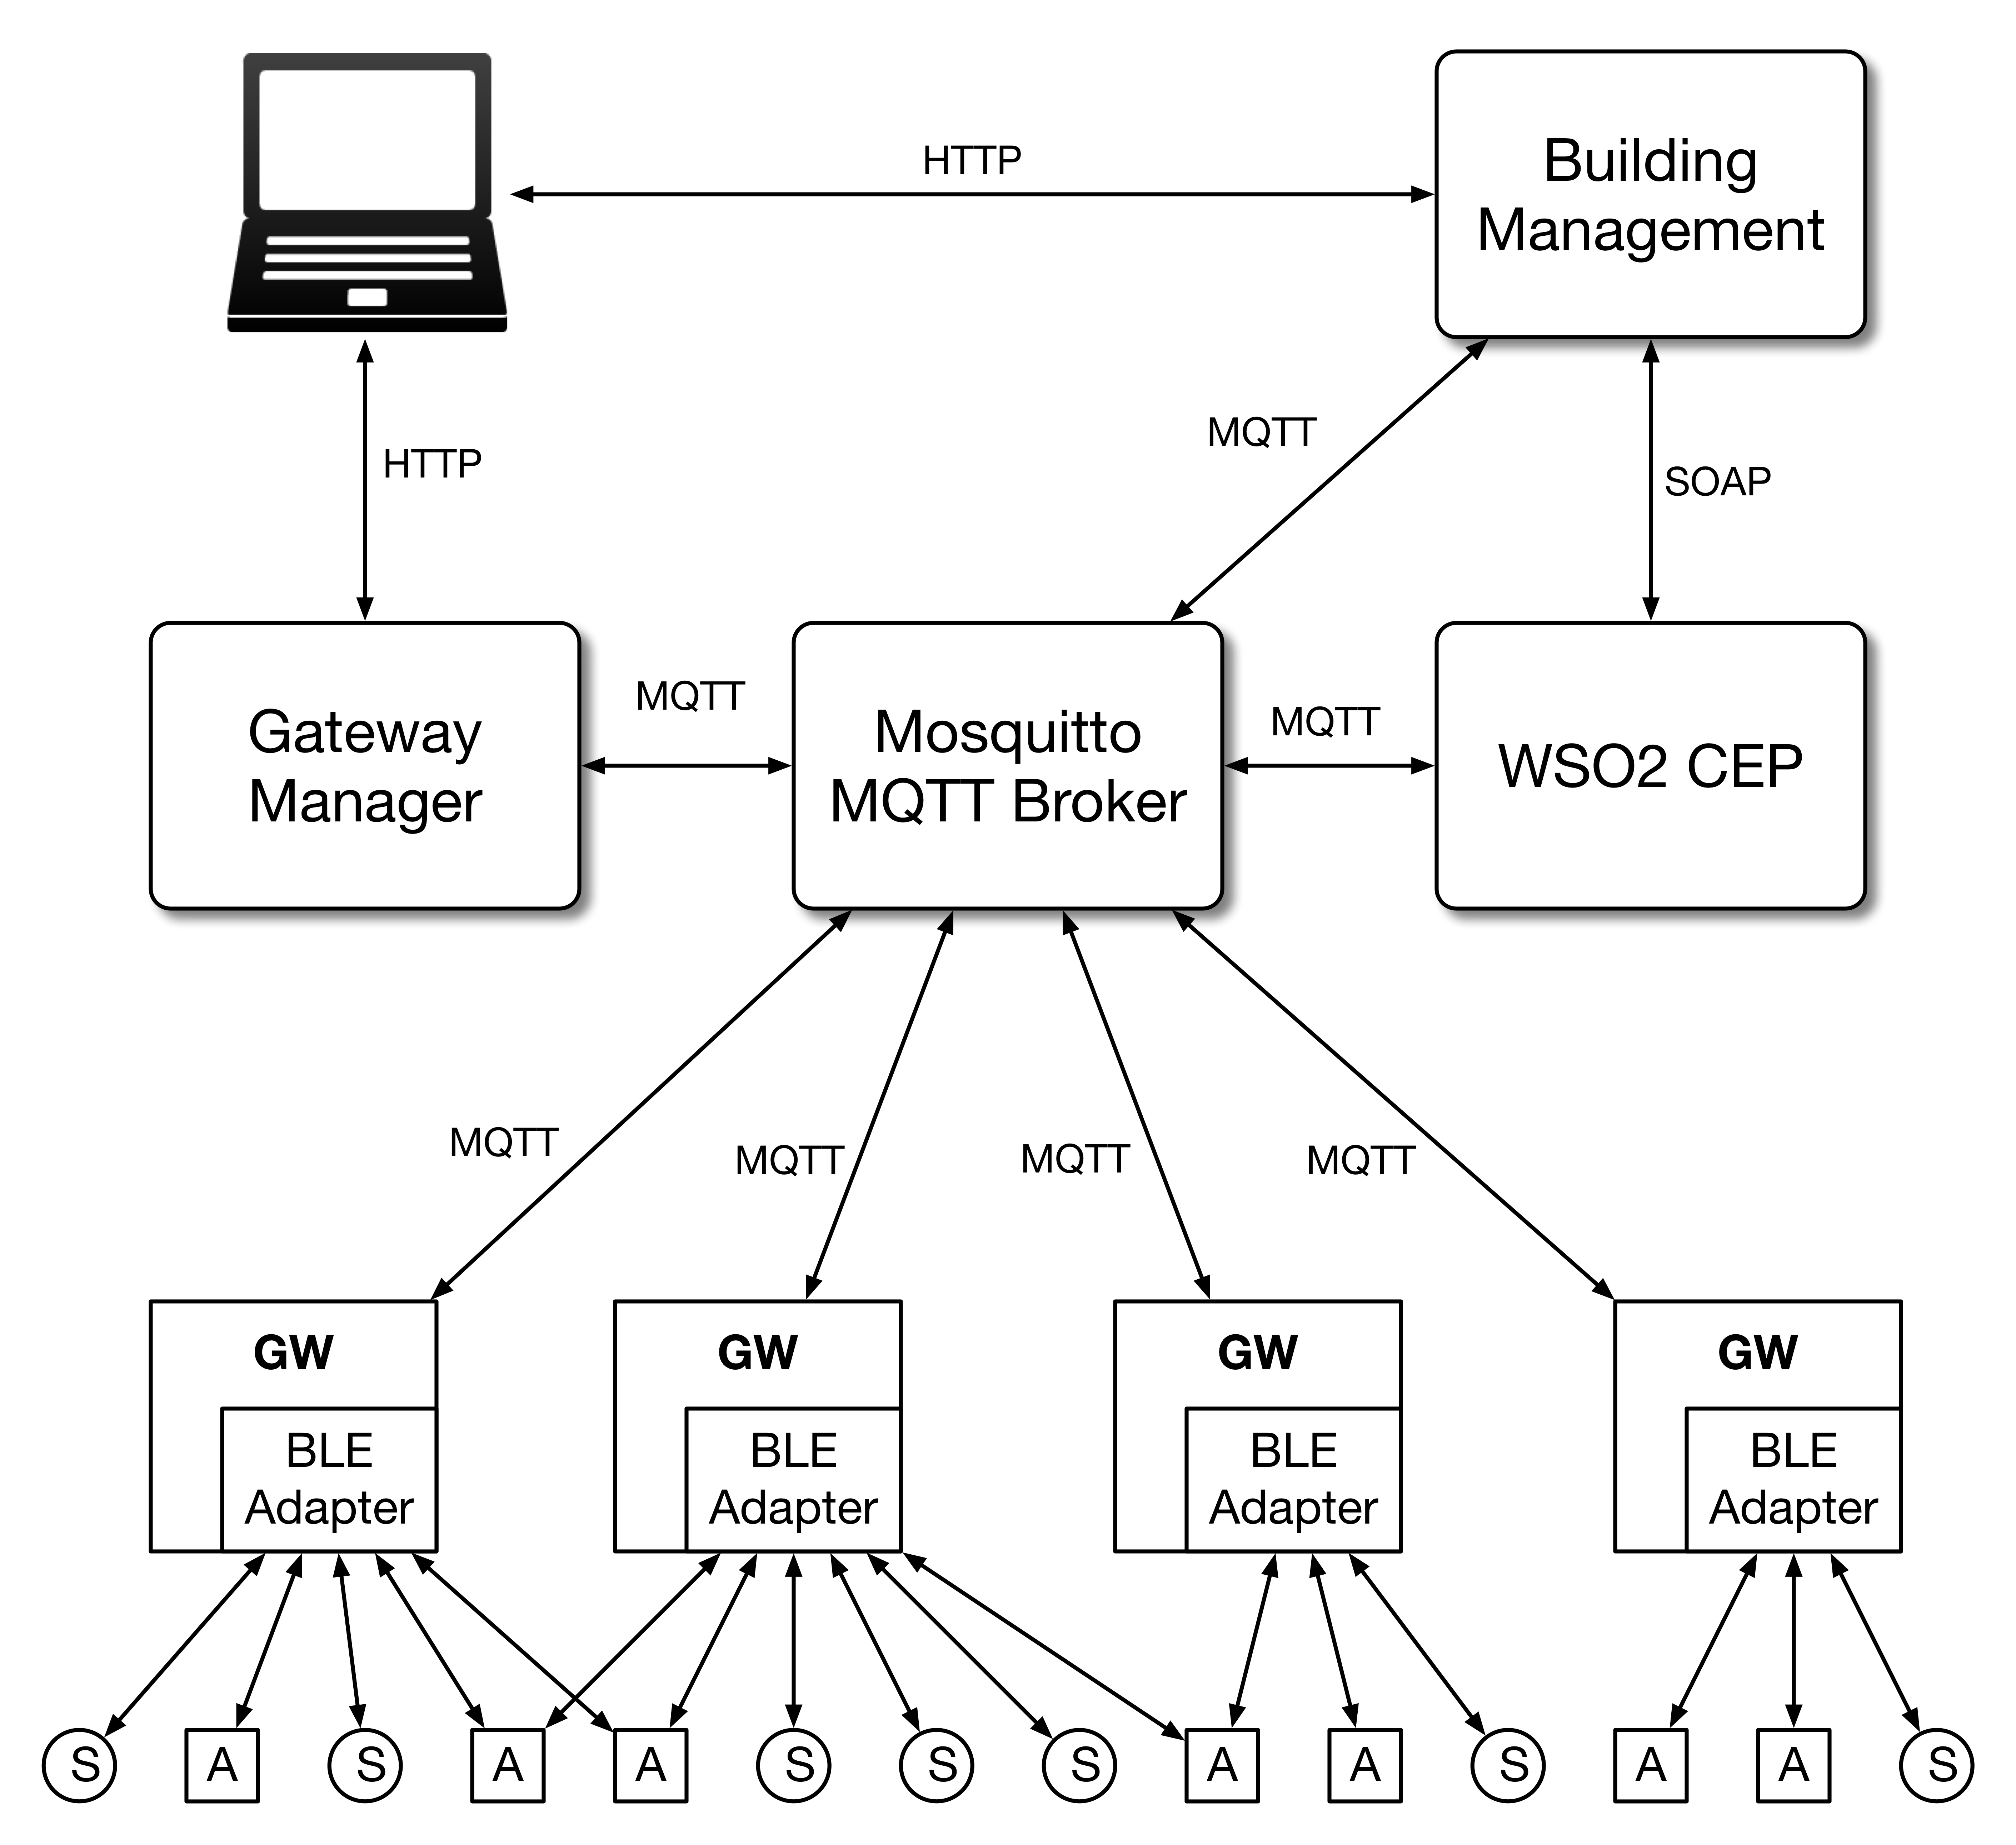
\includegraphics[width=0.8\textwidth]{figures/architecture3.png}
	\caption{Implementation Architecture}
	\label{fig:arch2}
\end{figure}

For the scope of this dissertation, the focus was the implementation of a Gateway with ability to configure and manage devices, and with a lightweight automation engine that is able to parse rules and process events based on them. Also it was implemented a Gateway Manager with features like rule parsing and distribution among gateways and failure handling and synchronization of gateways.

Regarding the failover strategy used, the detection of failures was insured by making every component report its state to the central broker, by publishing a periodic MQTT heart\_beat message. This way, if a fail occurs, the other working nodes are able to detect the absence of the failing node and begin recovering from the fault. All the processes regarding these features will be explained next.


\subsection{Gateway Manager}
\label{arch:gm}

This section will describe how the Gateway Manager fits in the fulfilment of the requirements and objectives proposed for this project, and also how its features were thought and implemented. 


This component was programmed using Python 3\footnote{https://docs.python.org/3/} and since MQTT was the chosen protocol to communicate with other nodes, the Eclipse Paho MQTT Python client\footnote{https://pypi.python.org/pypi/paho-mqtt/1.3.0} library was used. This client enables the application to connect to a MQTT broker in order to publish messages and subscribe to topics. Bellow will be described the most important features implemented for this component.


\begin{Paragraph}{Rule Parsing and Distribution}
	
One of the Gateway's Manager roles is to receive rules, developed in the existing Building Manager platform. As addressed before, a rule is represented in JSON format, and when the rule is set to be deployed in the gateway's automation engine, the Gateway Manager parses it in order to divide the rule in sub rules and distribute them among the available gateways. To keep track of which rules are deployed where, and to which rule's different targets and listeners correspond, the \ac{gm} attributes a unique ID to each rule and stores, in data structures, the topics(from input and output events) used in each rule and to which rule IDs they correspond, since different rules can have the same targets and/or listeners. These data structures will be important to implement the fail handling measures, which will be addressed later. In Figure \ref{fig:parser_struct}, can be observed the data structure used to store this information. Each entry in the list is a tuple containing a target topic(or listener topic) and a list of rules ID's that contain the same topic.

\begin{figure}[H]
	\centering
	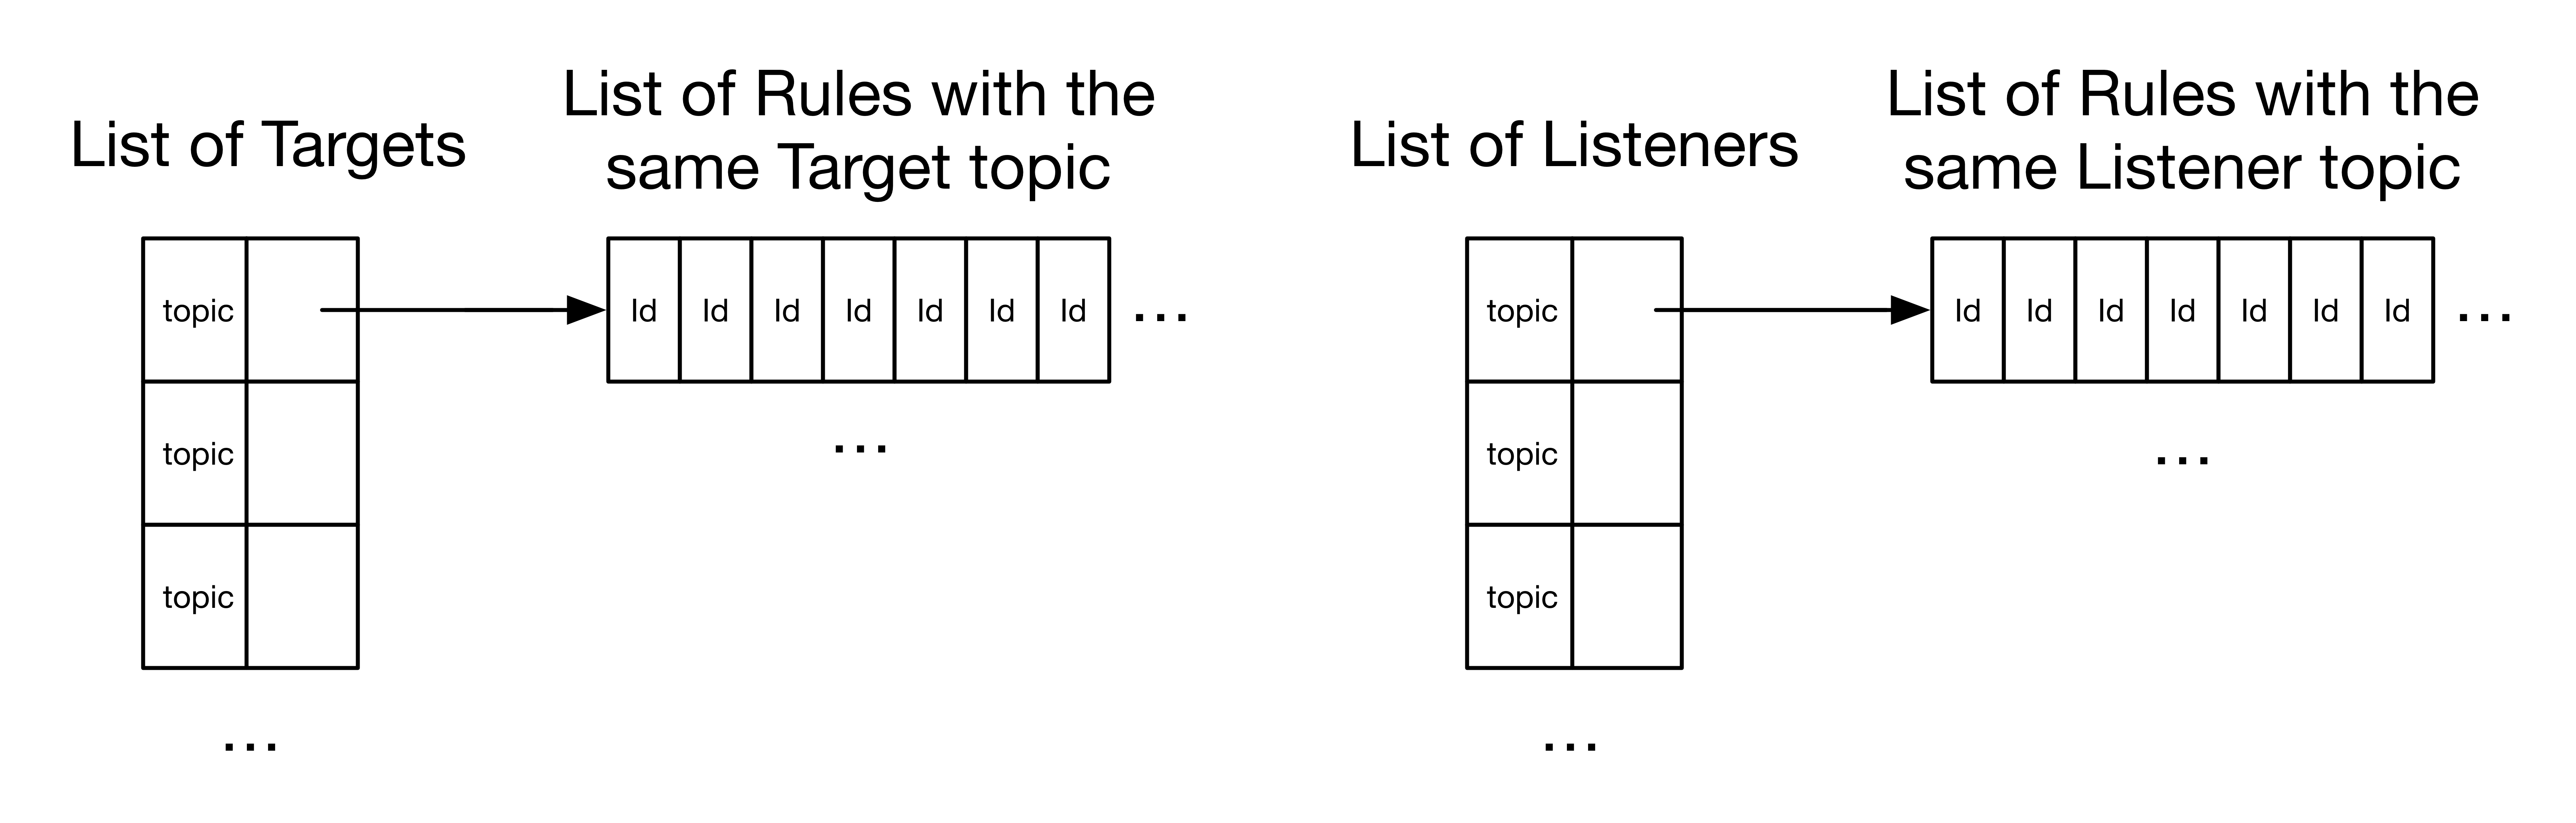
\includegraphics[width=0.9\textwidth]{figures/parser_struct.png}
	\caption{Data structures used to store Targets and Listeners and to which Rule IDs they correspond.}
	\label{fig:parser_struct}
\end{figure}

After the rule is parsed, the \ac{gm} distribute the sub rules to the available gateways using a round-robin method, in order to maintain a equal number or deployed rules among gateways. This approach was chosen so that gateways can have a balanced load between them. Other approaches could have been implemented, such as distribute rules by proximity to the devices that they refer to, but as downside, there could be gateways with an extensive number of rules that could put in jeopardy the performance and responsiveness of event processing. 

In Figure \ref{fig:addrule} can be observed an interaction diagram of the communication needed to add a new rule to the Gateway Manager and a Subrule to a Gateway, using MQTT.

\begin{figure}[H]
	\centering
	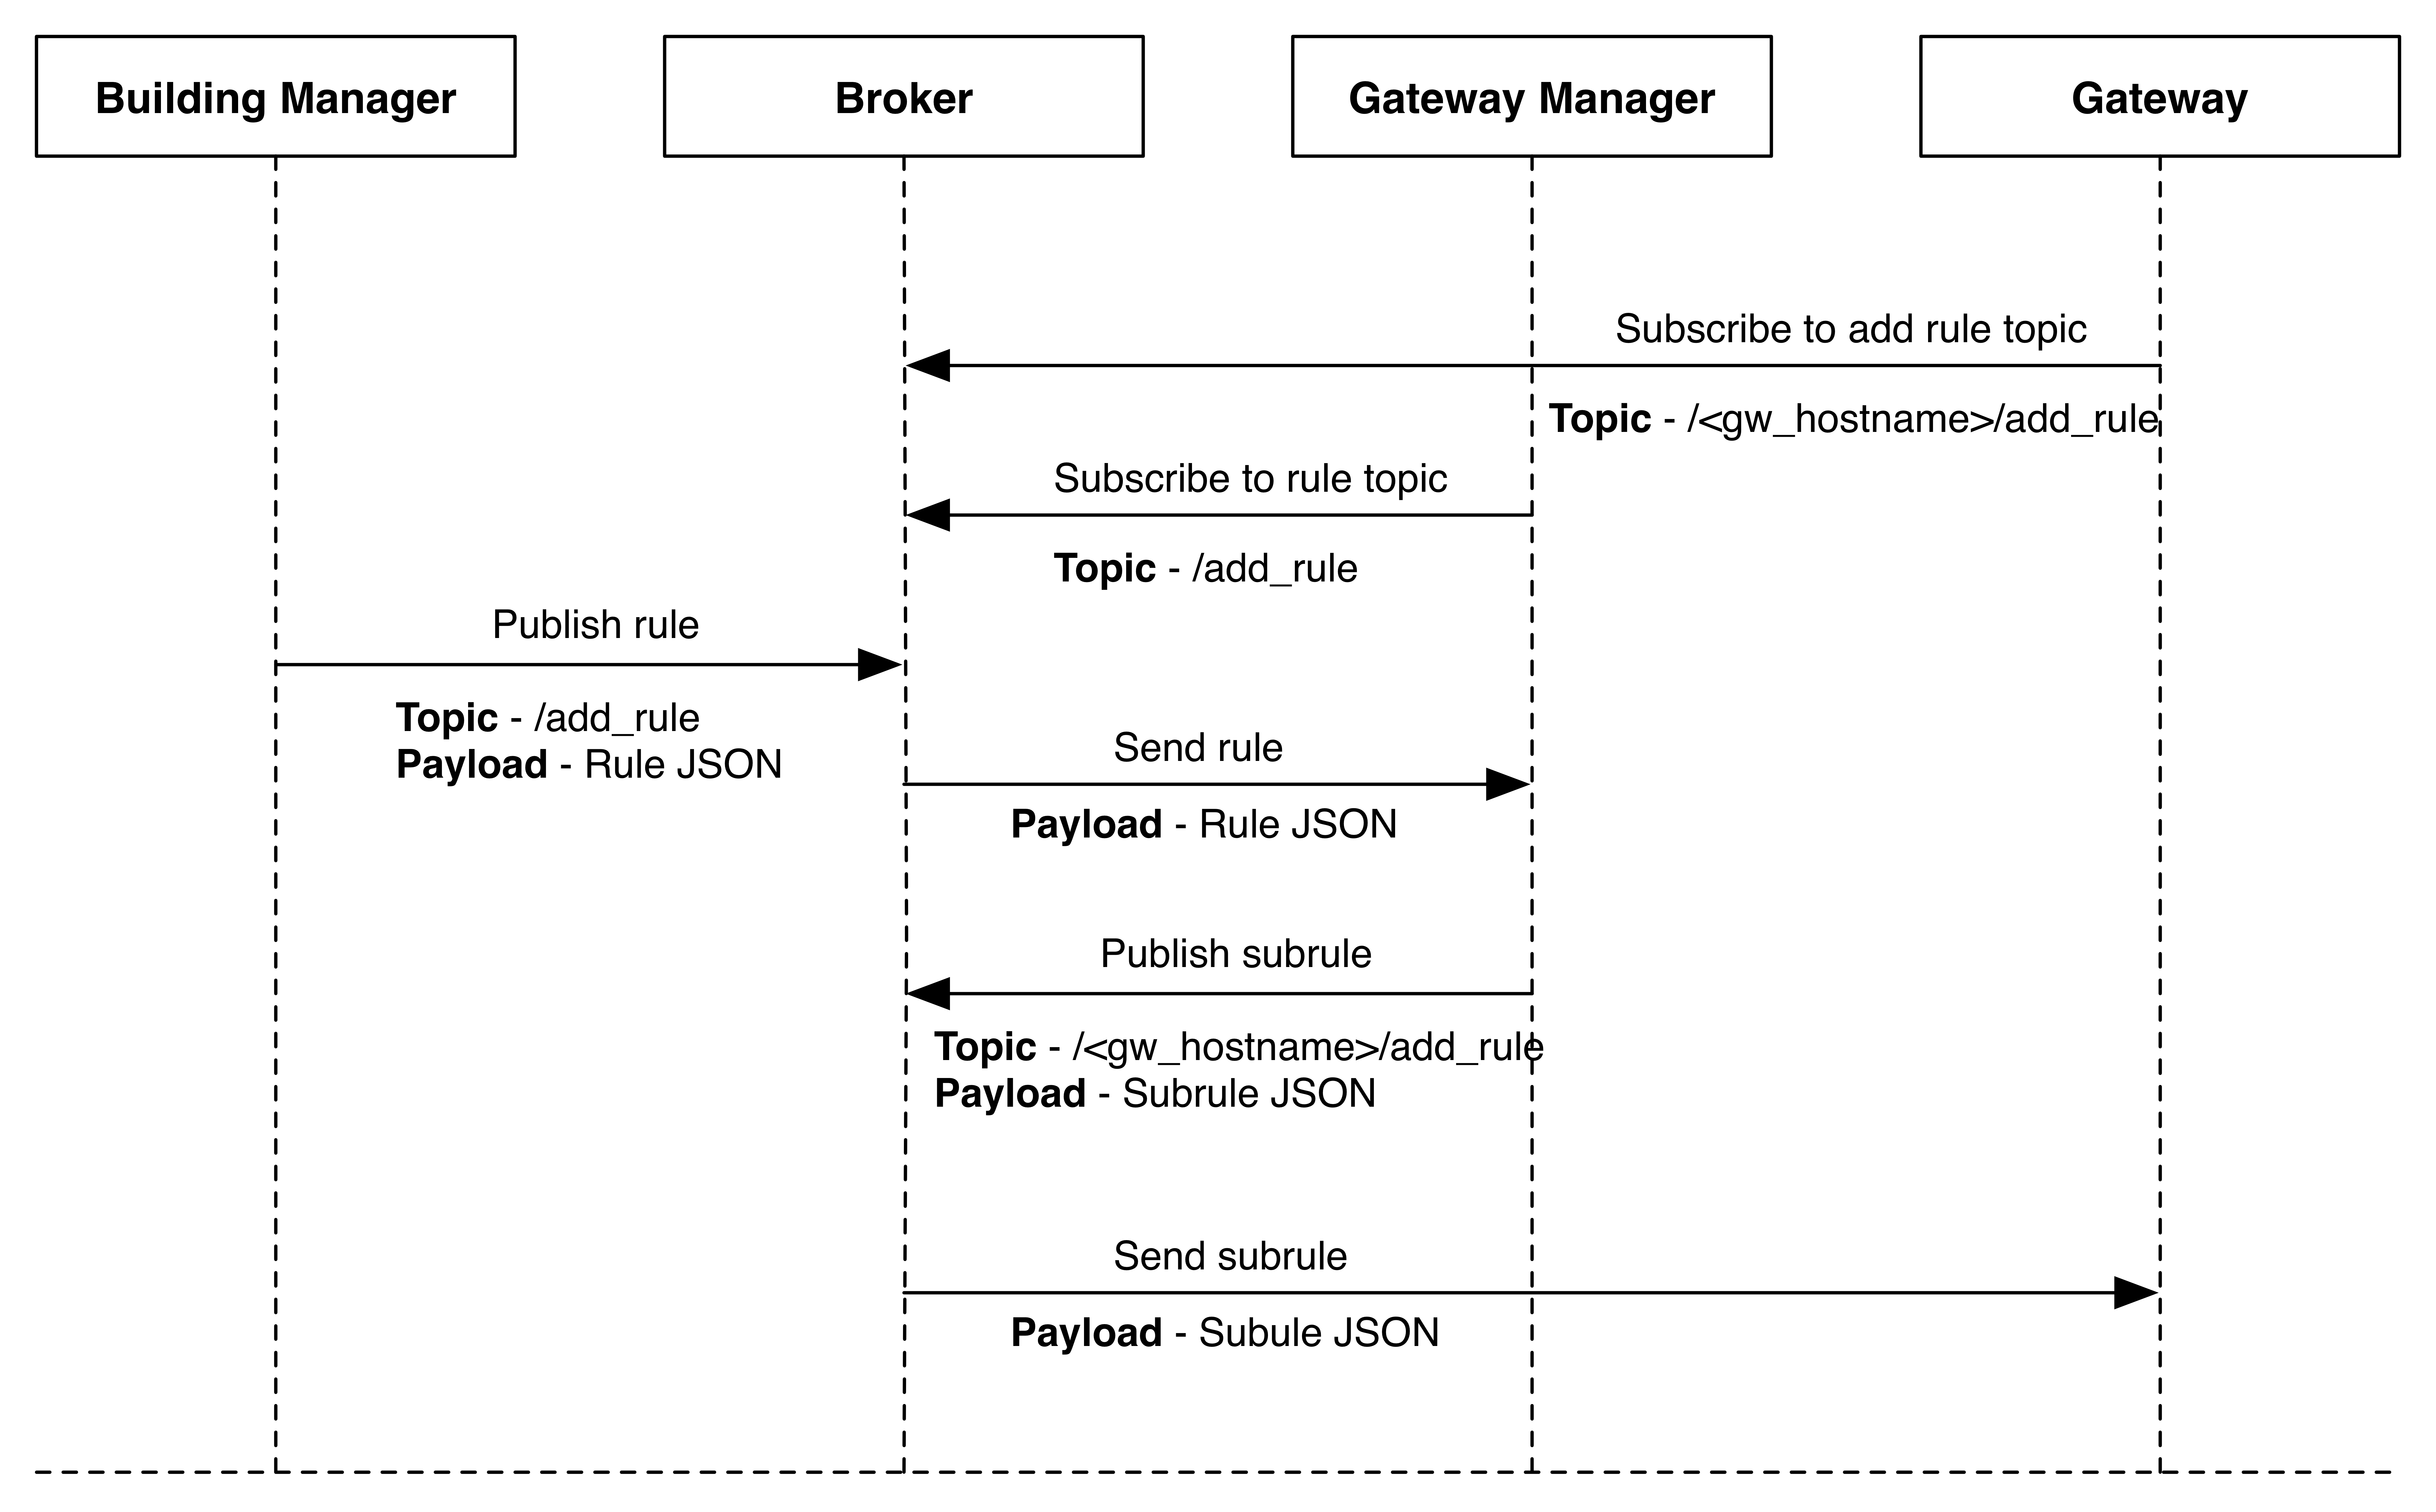
\includegraphics[width=0.9\textwidth]{figures/addrule.png}
	\caption{Interaction diagram of adding a new rule to the Gateway Manager and a Subrule to a Gateway.}
	\label{fig:addrule}
\end{figure}

As can be observed, the Building Manager publishes a rule and the Gateway Manager parses it in order to divide them into subrules. These subrules are numbered and then distributed to Gateways using the topic(already subscribed in the broker by Gateways) ``/<gw\_hostname>/add\_rule''.

\end{Paragraph}

\begin{Paragraph}{System Awareness}

The \ac{gm}, being the unit that will impose the fail handling measures, needs to be aware of each component and each gateway state. In order to do that, and as addressed before, each component has to send a periodic heart beat message to the central broker, using the ``/heart\_beat'' topic, which is subscribed by the \ac{gm}. The \ac{gm} then checks periodically if every component sent the heart\_beat. If a component fails and it is not able to send the heart\_beat, after a programmable timeout, the \ac{gm} begins the implementation of failing handling measures. These features could have been implemented using Last Will feature of MQTT. Clients could configure a Last Will message, so that upon disconnecting from the broker, due to a failure, that message would be published in the broker and the other nodes would be aware that the faulty node was disconnected. This approach was not implemented so that other protocols, such as COAP(that does not support this feature) could be used, without profound changes in the application's code.

\end{Paragraph}

\begin{Paragraph}{Devices Configuration}

When new a gateway is connected to the system, it sends a message to the \ac{gm}, informing which devices it is able to connect and then, with this information, the \ac{gm} balances the available devices among the gateways. To explain further, when two gateways are able to connect to the same devices, the \ac{gm} balances that devices among the two in order to maintain a equal number of devices in each one. Also, it stores for each device, the gateways that are able to connect to it. This allows that when a gateway fails, the \ac{gm} has all the information needed to inform the gateways that are able to connected to the lost devices, to take control of those devices.

\end{Paragraph}

\begin{Paragraph}{Gateway Manager Dashboard}

In order to visualize the state of the gateways present in the system, a dashboard was created, using Python3 web framework Flask\footnote{http://flask.pocoo.org/}. In Figure \ref{fig:main_gm} is shown the main page of this dashboard.

\begin{figure}[H]
	\centering
	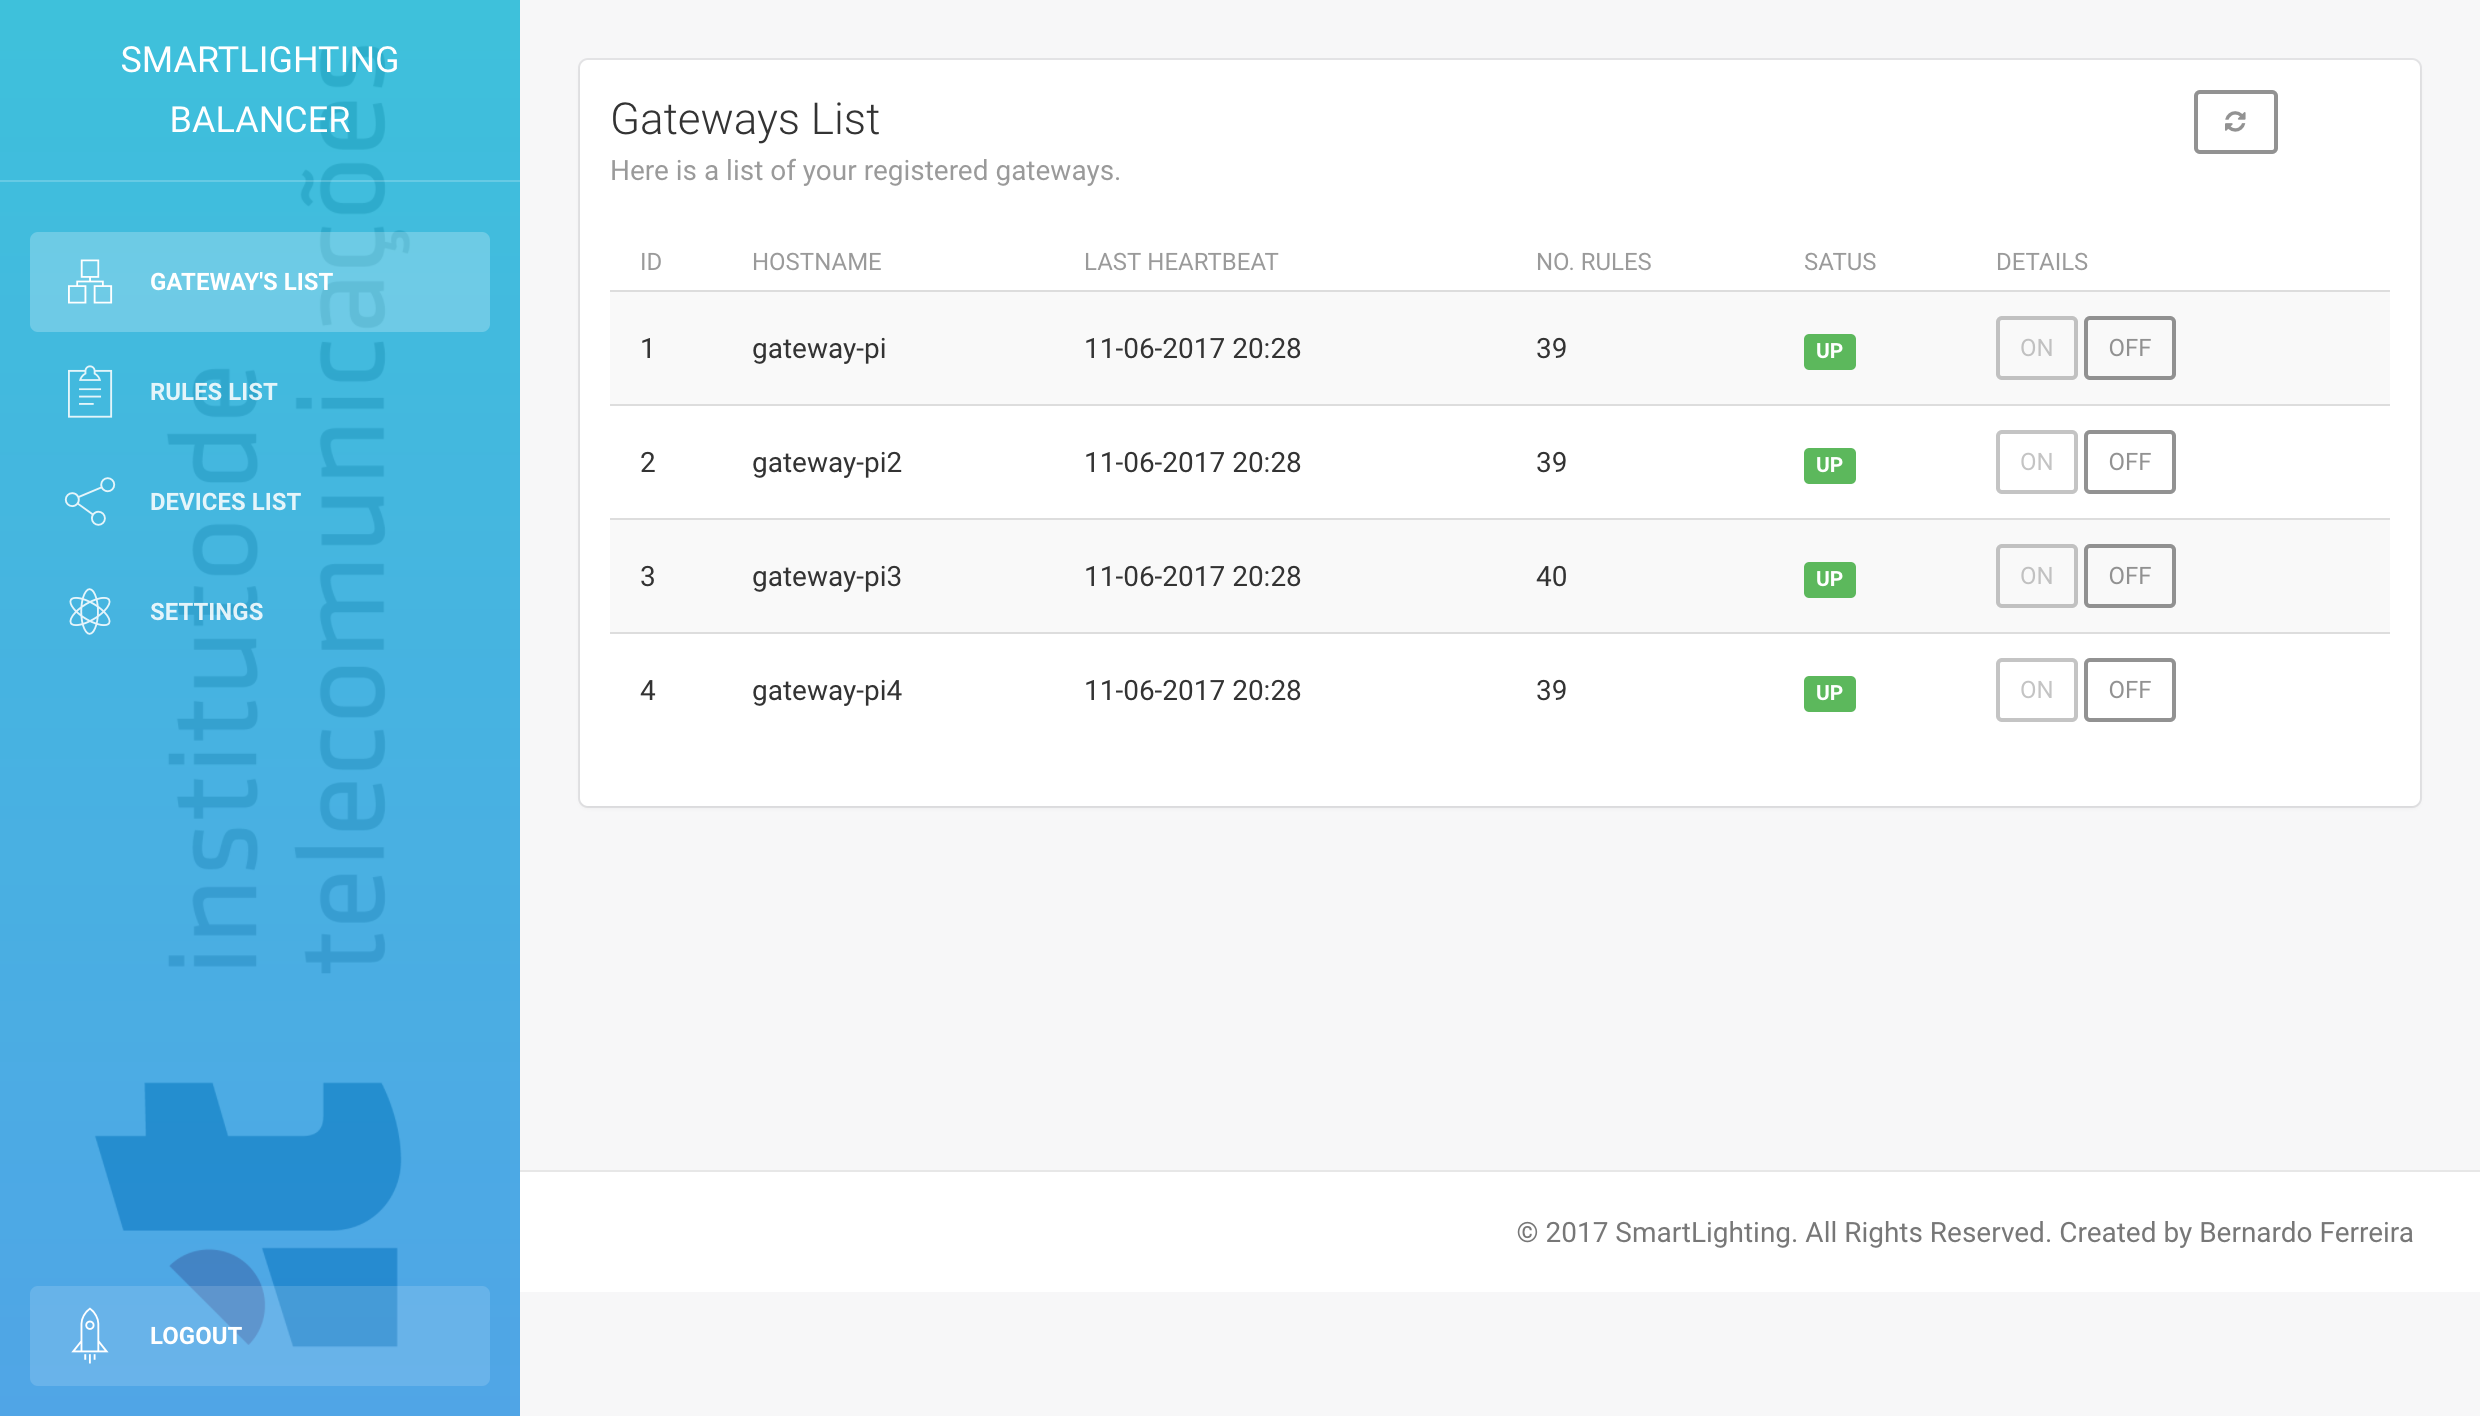
\includegraphics[width=0.9\textwidth]{figures/main_gm.png}
	\caption{Screenshot of the Gateway Manager dashbord main page.}
	\label{fig:main_gm}
\end{figure}

As can be observed, this dashboard allows to check several information about the gateways, such as, the hostnames, the time of the last heart beat received, the number of devices connected, and has also a feature to turn on/off a gateway if pleased. Also, it has not only the the list of rules and in which gateway they are being deployed, but also a list of devices and the corresponding gateway.


\end{Paragraph}

\begin{Paragraph}{Gateway Failure Handling}
	
Since Gateways are the components that communicate directly with devices, a gateway failure could have a huge impact for the building. For that reason, one of the most important features of the \ac{gm} is to detect that a gateway fails and, as addressed before, inform other gateways within the range of the lost devices to assume control. Also, the rules that were present in the failing gateway, should also be sent to other gateways to be deployed. Bellow in Figure \ref{fig:gwdown}, it is represented the interaction diagram of the processes that occur when a gateway fails. 

\begin{figure}[H]
	\centering
	\includegraphics[width=0.9\textwidth]{figures/gwdown.png}
	\caption{Interaction diagram of the procedures when a gateway fails.}
	\label{fig:gwdown}
\end{figure}
	
As can be observed, since the \ac{gm} has the information regarding which gateways have access to which devices, it can easily distribute the lost devices among the gateways that can communicate with them. Also, the rules that were deployed in the lost gateway are distributed through the available gateways using, again, a "round-robin" method in order to balance the number of rules in each gateway.  

\end{Paragraph}

\begin{Paragraph}{Gateways Synchronization}

In some cases, there can be an emergency where the gateways cannot send events nor receive actions through the central \ac{mqtt} Broker. In this state, Gateways must communicate directly with each others. In order to to that, not only they need to know to which gateways they should send its device events to be processed, but also need to know where they must send the processed events to. Since the Gateway Manager has all the information regarding the gateways state, i.e, which rules and devices are deployed in each gateway, the \ac{gm} generates, everytime there is a change in either a gateway's devices or rules, two JSON's containing this information and send them to all Gateways. The first JSON contains a list of Listeners \ac{mqtt} topics and for each one, a list of gateways that have process rules for those events. To explain further, when a device generates an event, the corresponding Gateway, uses the information in this JSON to know which gateways are deploying rules that process that event, and send it to each one of them. The second JSON contains a list of Targets and the respective gateways that have devices triggered by that output event. This way, when a gateway finishes the processing of an event, it finds in this list which gateways have devices that are triggered by that event and sends it to them.
 
\end{Paragraph}


\subsection{Gateway}
\label{arch:gw}

This section will describe how the Gateway proposed features and its requirements were implemented. Since this project aims to create a smart environment in buildings, the amount of gateways needed to cover the whole network of devices may vary depending on the building size. Most solutions in the \ac{bas} systems rely on expensive gateways which can be a downside for stakeholders. The solution is to create a gateway software that is able to work in a microcontroller or in a small and cheap \ac{soc} like a Raspberry Pi\footnote{https://www.raspberrypi.org/} or a Nano Pi\footnote{http://www.nanopi.org/}. In an initial state, the implementation began to be done using Java, however, the program would consume too much memory, which would be a downside, taking into account the proposed requirements. With this in mind, the programming language used in the deployment of this software was MicroPython\footnote{https://micropython.org/}. MicroPython is an open source Python programming language interpretor that runs on small embedded development boards \cite{micro2} and, although being full packed with advanced features, it is compact enough run within just 256k of code space and 16k of RAM \cite{micro}. For these reasons, MicroPython was chosen to allow more flexibility when choosing gateway's hardware.

To allow the communication between gateways in a scenario where the access to the central \ac{mqtt} broker might be impossible, either due to a failure in the network or in the broker itself, a Mosquitto lightweight MQTT broker was also deployed in each gateway. The use for these brokers will be explained later in section \ref{implementation:scenarios}. Also, since the IP addresses of the several components, which are needed to communicate with each others, can change due to network problems, it was deployed in each node of the system an Avahi \acf{mdns} deamon\footnote{https://www.avahi.org/}, enabling that each component could be reached by just its hostname, which never changes for each machine.


\begin{Paragraph}{Devices Configuration and Management}

When a gateway is deployed, it needs to send, to the \ac{gm} a list of devices within its range and the resources that each device has. Later, the \ac{gm}, responds with a list of which devices should be controlled by the gateway and in which topics should gateways publish events generated by the devices. Also, gateways receive information concerning to which topics they must subscribe in the central broker. To explain further, gateways need to know in which topic to publish events, generated by each device, in the central broker. Also, after those events being processed in the CEP Engine, gateways need to be subscribed to the output event topics that concern the devices it controls, in order to receive the automation actions. Bellow, in Figure \ref{fig:newdevice}, is represented the interaction diagram of the communications needed to configure a new device. 


\begin{figure}[H]
	\centering
	\includegraphics[width=0.9\textwidth]{figures/newdevice.png}
	\caption{Interaction diagram of a new device configuration.}
	\label{fig:newdevice}
\end{figure}


	
\end{Paragraph}
\newpage

\begin{Paragraph}{Rule Parser}

The \ac{gm}, as addressed before, parses the received rules and give an unique ID to each subrule. Then, when balancing the rules among the available gateways, it sends a JSON with the subrule and the given ID. When a sub rule is received in a gateway, it must be deconstructed in order for the automation engine to know which events trigger it, and what actions must be performed. In Figure \ref{fig:parse} it is represented a flow diagram explaining the process of parsing a rule. As addressed before, each subrule can either have a Set Value or a Set Percent Function. In Set Value Functions, there is only one action to be parsed, however, in Set Percent Functions, there are two actions to be considered, a ``Listen\_value'' and a ``Listen\_boolean'' action. For each action, the parser checks the existence of the modules addressed before, i.e. Windows, Aggregators, Filters and Converters, and creates an object for each one of them, containing its informations. An Action object is then created, containing an unique ID and a reference for the modules objects. In the end, the parser saves in a data structure, the information regarding the rule in the following way: ``Rules[Listeners] = [ActionsID]'', where, Rules is a list of MQTT topics, of the different listeners parsed, and each one of them has a list of ActionsIDs with the same Listener. This was implemented this way so that when an event is received, it is only needed to search for the corresponding Listener topic, in the data structure, to know which actions must be triggered. 


\begin{figure}[H]
	\centering
	\includegraphics[width=0.7\textwidth]{figures/parseRule.png}
	\caption{Rule parser flow diagram}
	\label{fig:parse}
\end{figure}

\end{Paragraph}

\begin{Paragraph}{Gateway Automation Engine}

The \acf{gae}, as stated before, will only work in emergency states, either if the central broker or the \ac{cep} Engine are down. When this happens, gateways subscribe, in the central broker, to the MQTT topics of the listeners present in the rules deployed by each one. This way, the events generated by the devices are published in the broker and then sent to gateways that have rules with those events as input for its rules. 

As mentioned earlier, when an event arrives to a gateway, first it must discover the Actions that need to be triggered so that the event can be processed. The \ac{gae} was designed to implement the modules present in Table \ref{module-table}.
 
\begin{table}[H]

	\resizebox{\textwidth}{!}{\begin{tabular}{|c|c|l|}
		\hline
		\textbf{Type}               & \textbf{Module}       & \textbf{Description}                                                                                                                                            \\ \hline
		Listener                    & MQTT                  & MQTT topic to receive events                                                                                                                                     \\ \hline
		Target                      & MQTT                  & MQTT topic to send events                                                                                                                                        \\ \hline
		\multirow{2}{*}{Function}   & Set Value             & Set the value received from input streams to the output streams                                                                                                 \\ \cline{2-3} 
		& Set Percent           & \begin{tabular}[c]{@{}l@{}}Set a percentage of a value from input streams to the output\\ streams, based on boolean data from another input stream\end{tabular} \\ \hline
		\multirow{6}{*}{Filter}     & Equal                 & Filter events with the value equal to a given value                                                                                                             \\ \cline{2-3} 
		& Not Equal             & Filter events with the value different than a given value                                                                                                       \\ \cline{2-3} 
		& Greater Than          & Filter events with the value greater than a given value                                                                                                         \\ \cline{2-3} 
		& Less Than             & Filter events with the value less than a given value                                                                                                            \\ \cline{2-3} 
		& Greater or Equal Than & Filter events with the value greater or equal to a given value                                                                                                  \\ \cline{2-3} 
		& Less or Equal Than    & Filter events with the value less or equal to a given value                                                                                                     \\ \hline
		\multirow{2}{*}{Window}     & Time Window           & Capture events in a predefined time                                                                                                                             \\ \cline{2-3} 
		& Length Window         & Capture a predefined number of events                                                                                                                           \\ \hline
		\multirow{3}{*}{Aggregator} & Average               & Calculate the average value of all the events in a window                                                                                                       \\ \cline{2-3} 
		& Any                   & Returns 1 if any of the values in the window is greater than 0                                                                                                  \\ \cline{2-3} 
		& None                  & Returns 1 if all the values in a window are 0                                                                                                                   \\ \hline
		\multirow{3}{*}{Converter}  & Lux To Percentage     & \begin{tabular}[c]{@{}l@{}}Calculates an output percentage value to apply on a luminaire’s\\ dimming level based on a value in lux units\end{tabular}           \\ \cline{2-3} 
		& Set 1                 & Sets the value to 1                                                                                                                                             \\ \cline{2-3} 
		& Set 0                 & Sets the value to 0                                                                                                                                             \\ \hline
	\end{tabular}}
	\centering
\caption{Implemented modules in Gateway's automation engine.}
\label{module-table}
\end{table}

For each action, the \ac{gae} follows certain steps, as can be visualized in Figure's \ref{fig:action} flow diagram. The first module to be applied is the Filter, if present in the action. If the value present in the event does not pass the filter verification is automatically discarded. After that, the \ac{gae} checks if the action has a window, and as consequence an aggregator, and if so, which type of window and applies it. For instance, with a Time Window with an Any Aggregator, the program must send the value 1 and, if no other event is received within the window time length, the \ac{gae} must send a value 0. If a new event is received within the time window length, the old window is discarded and begins a timer for the new one. Since micropython is a single-threaded programming language, in order to implement features like this one, it had to be used an event pool, in which, each event received is added as a new task for the event pool, and this way, to implement the time window, per example, is only needed to put the task of that event to sleep, the expected time length. Meanwhile the program can run and process other events present in the pool. The implementation of the Time Window module can is represented in Snippet \ref{snippet:rule} in Appendix B. Lastly, the Converter module, if present, processes the value based on the converting rules given and an event is sent to the central broker. 

This automation engine will only be enabled if the \ac{cep} Engine or the central broker fail, as will be addressed and explained later.

\begin{figure}[]
	\centering
	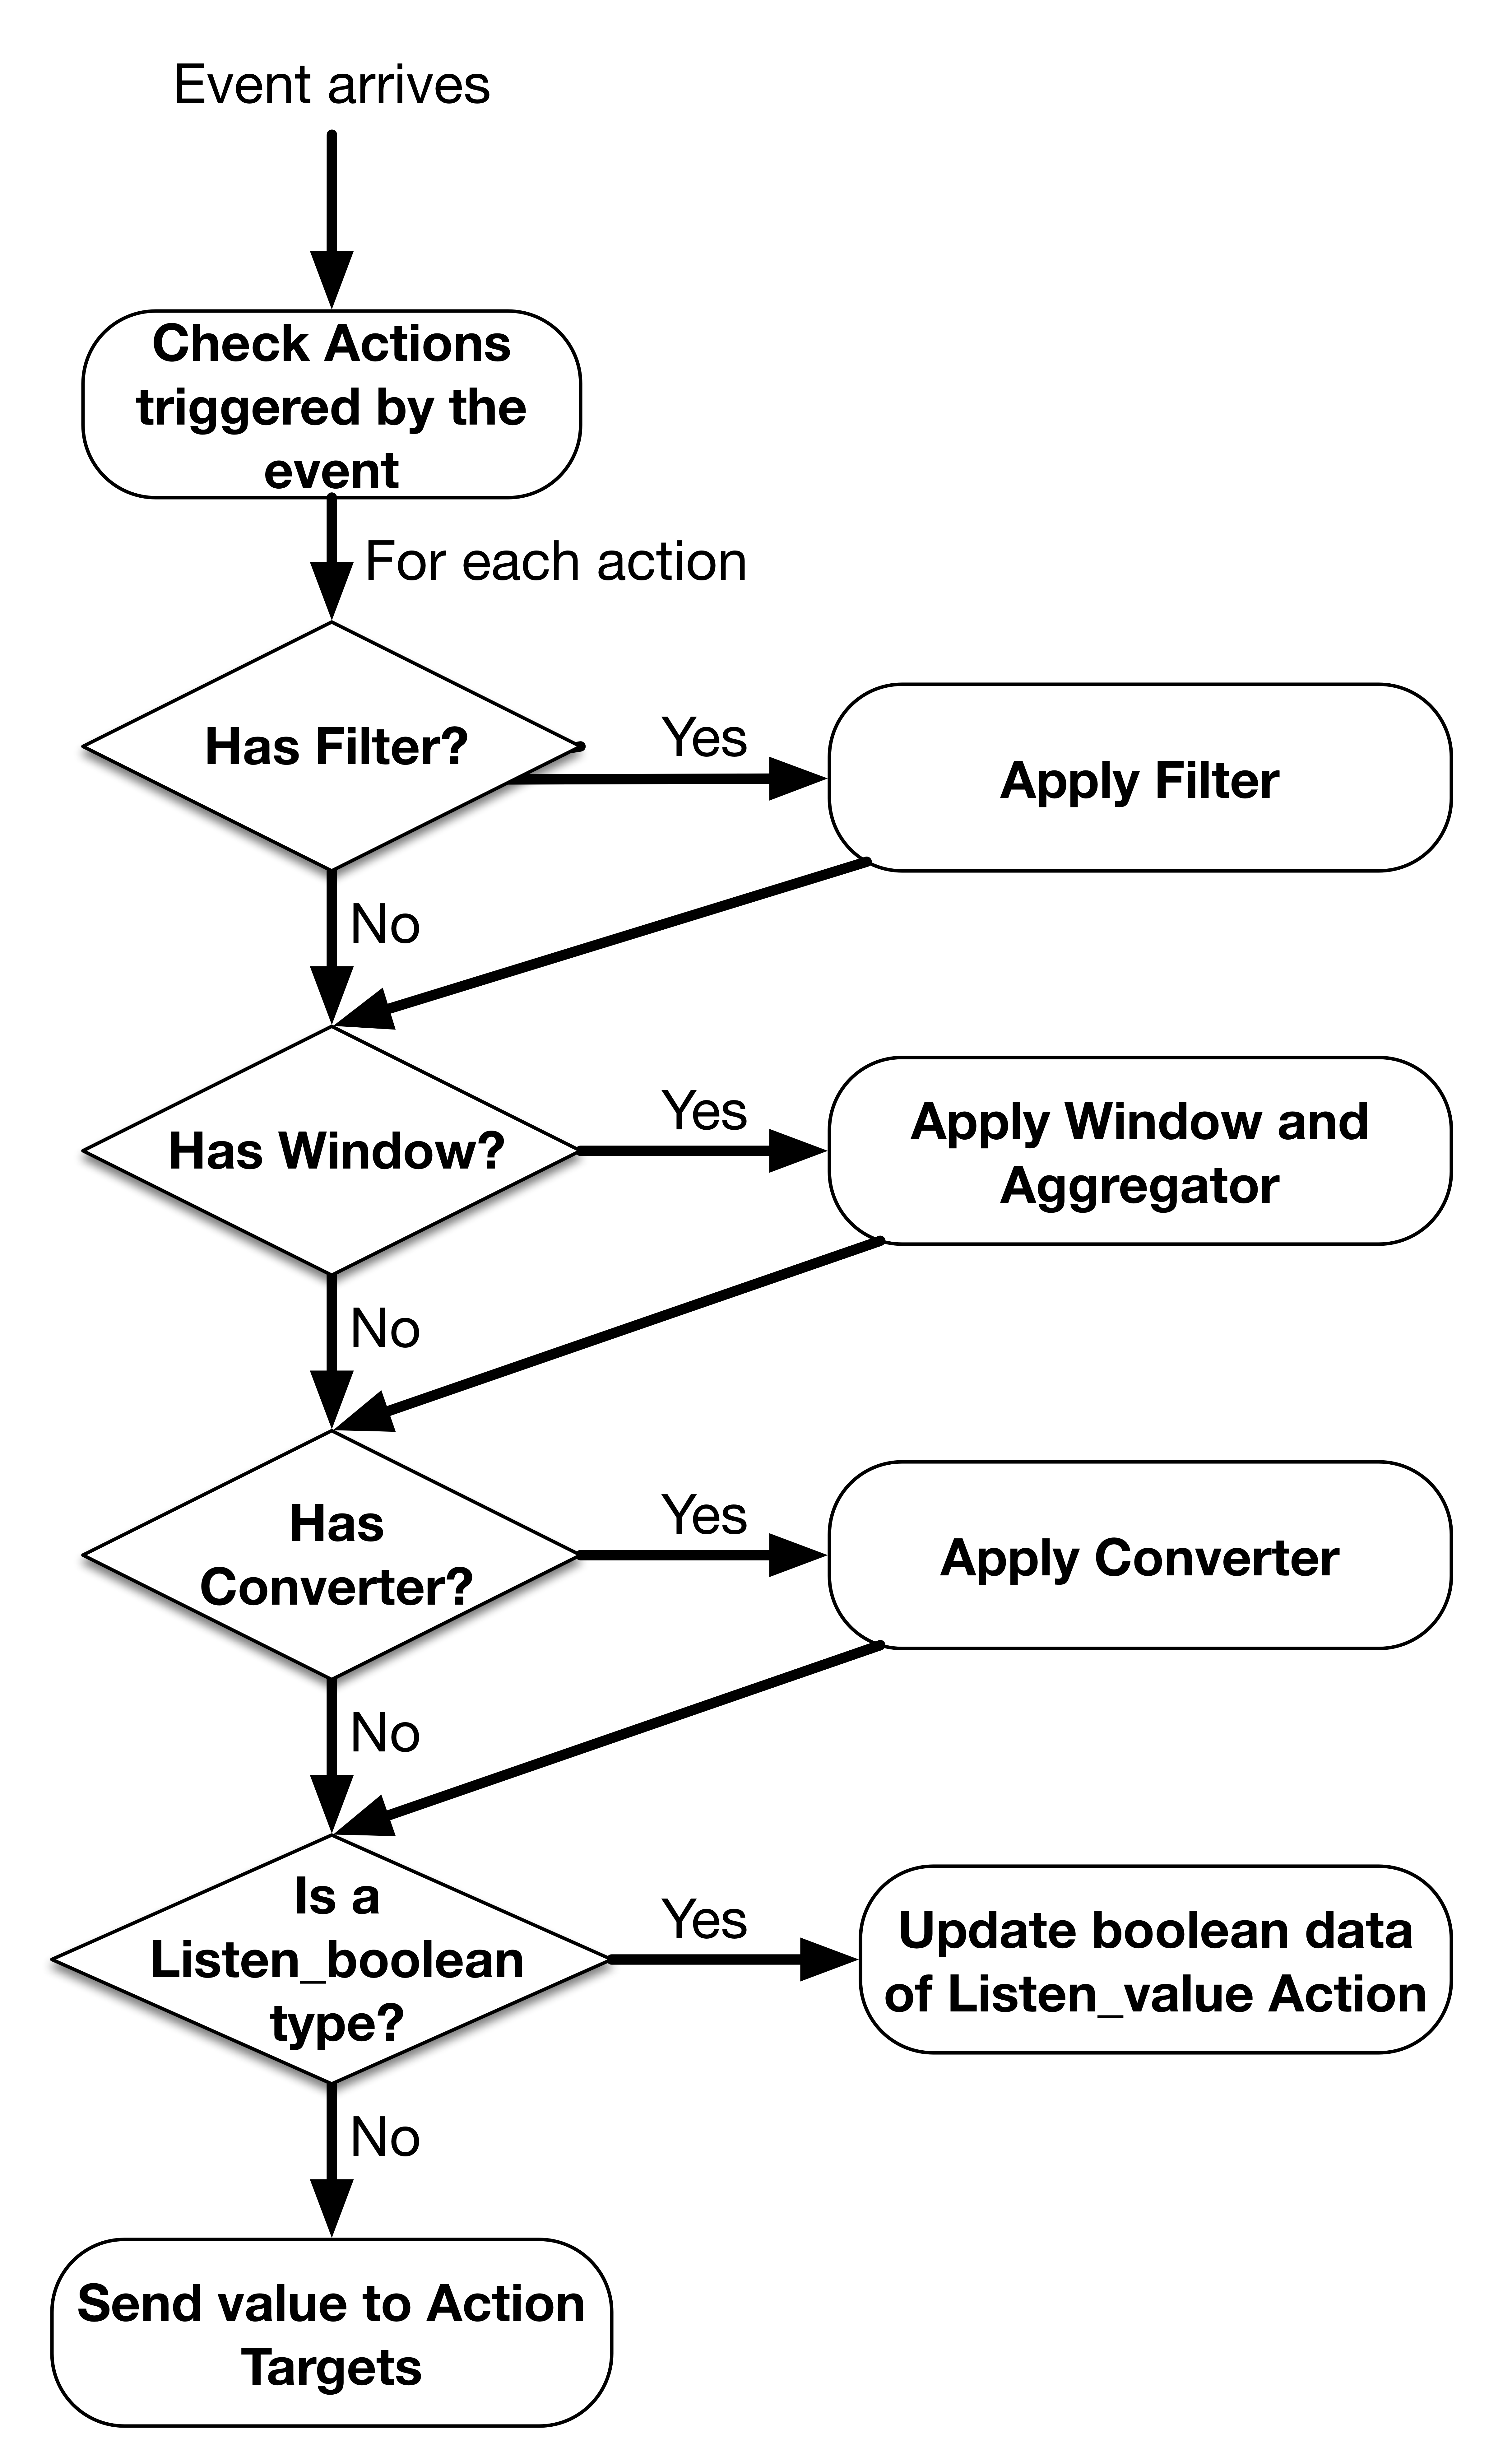
\includegraphics[width=0.6\textwidth]{figures/action.png}
	\caption{Event processing flow diagram.}
	\label{fig:action}
\end{figure}

\end{Paragraph}

\section{Functioning Scenarios}
\label{implementation:scenarios}

As one of the most important requirements and objectives for the present dissertation project, the fail handling mechanisms are a core feature for every smart environment deployed in a building. In order to rely with assurance in a fully autonomous system, it must be adapted to answer swiftly to unexpected behaviours within the system. In the scope of this project, the most important component, to impose an autonomous system, is the \ac{cep} engine, however if that component fails, due to internal software failure or a communication failure, the integrity of the building as well as the safety of its occupants could be at risk. For this reason, as addressed before, an automation engine (\ac{gae}) was implemented so that gateways could process events in order to trigger actions.

In section \ref{Architecture:usecases}, were introduced five different functioning scenarios: every component working as expected, \ac{cep} Engine down, Gateway Manager down, both CEP Engine and Gateway Manager down, and lastly, the MQTT broker down. For each of these scenarios, it will be explained how the system handle each of the failures in order to maintain the minimum functionalities of the building. 
\begin{Paragraph}{Scenario 1 - All components are operational}
\begin{figure}[H]
	\centering
	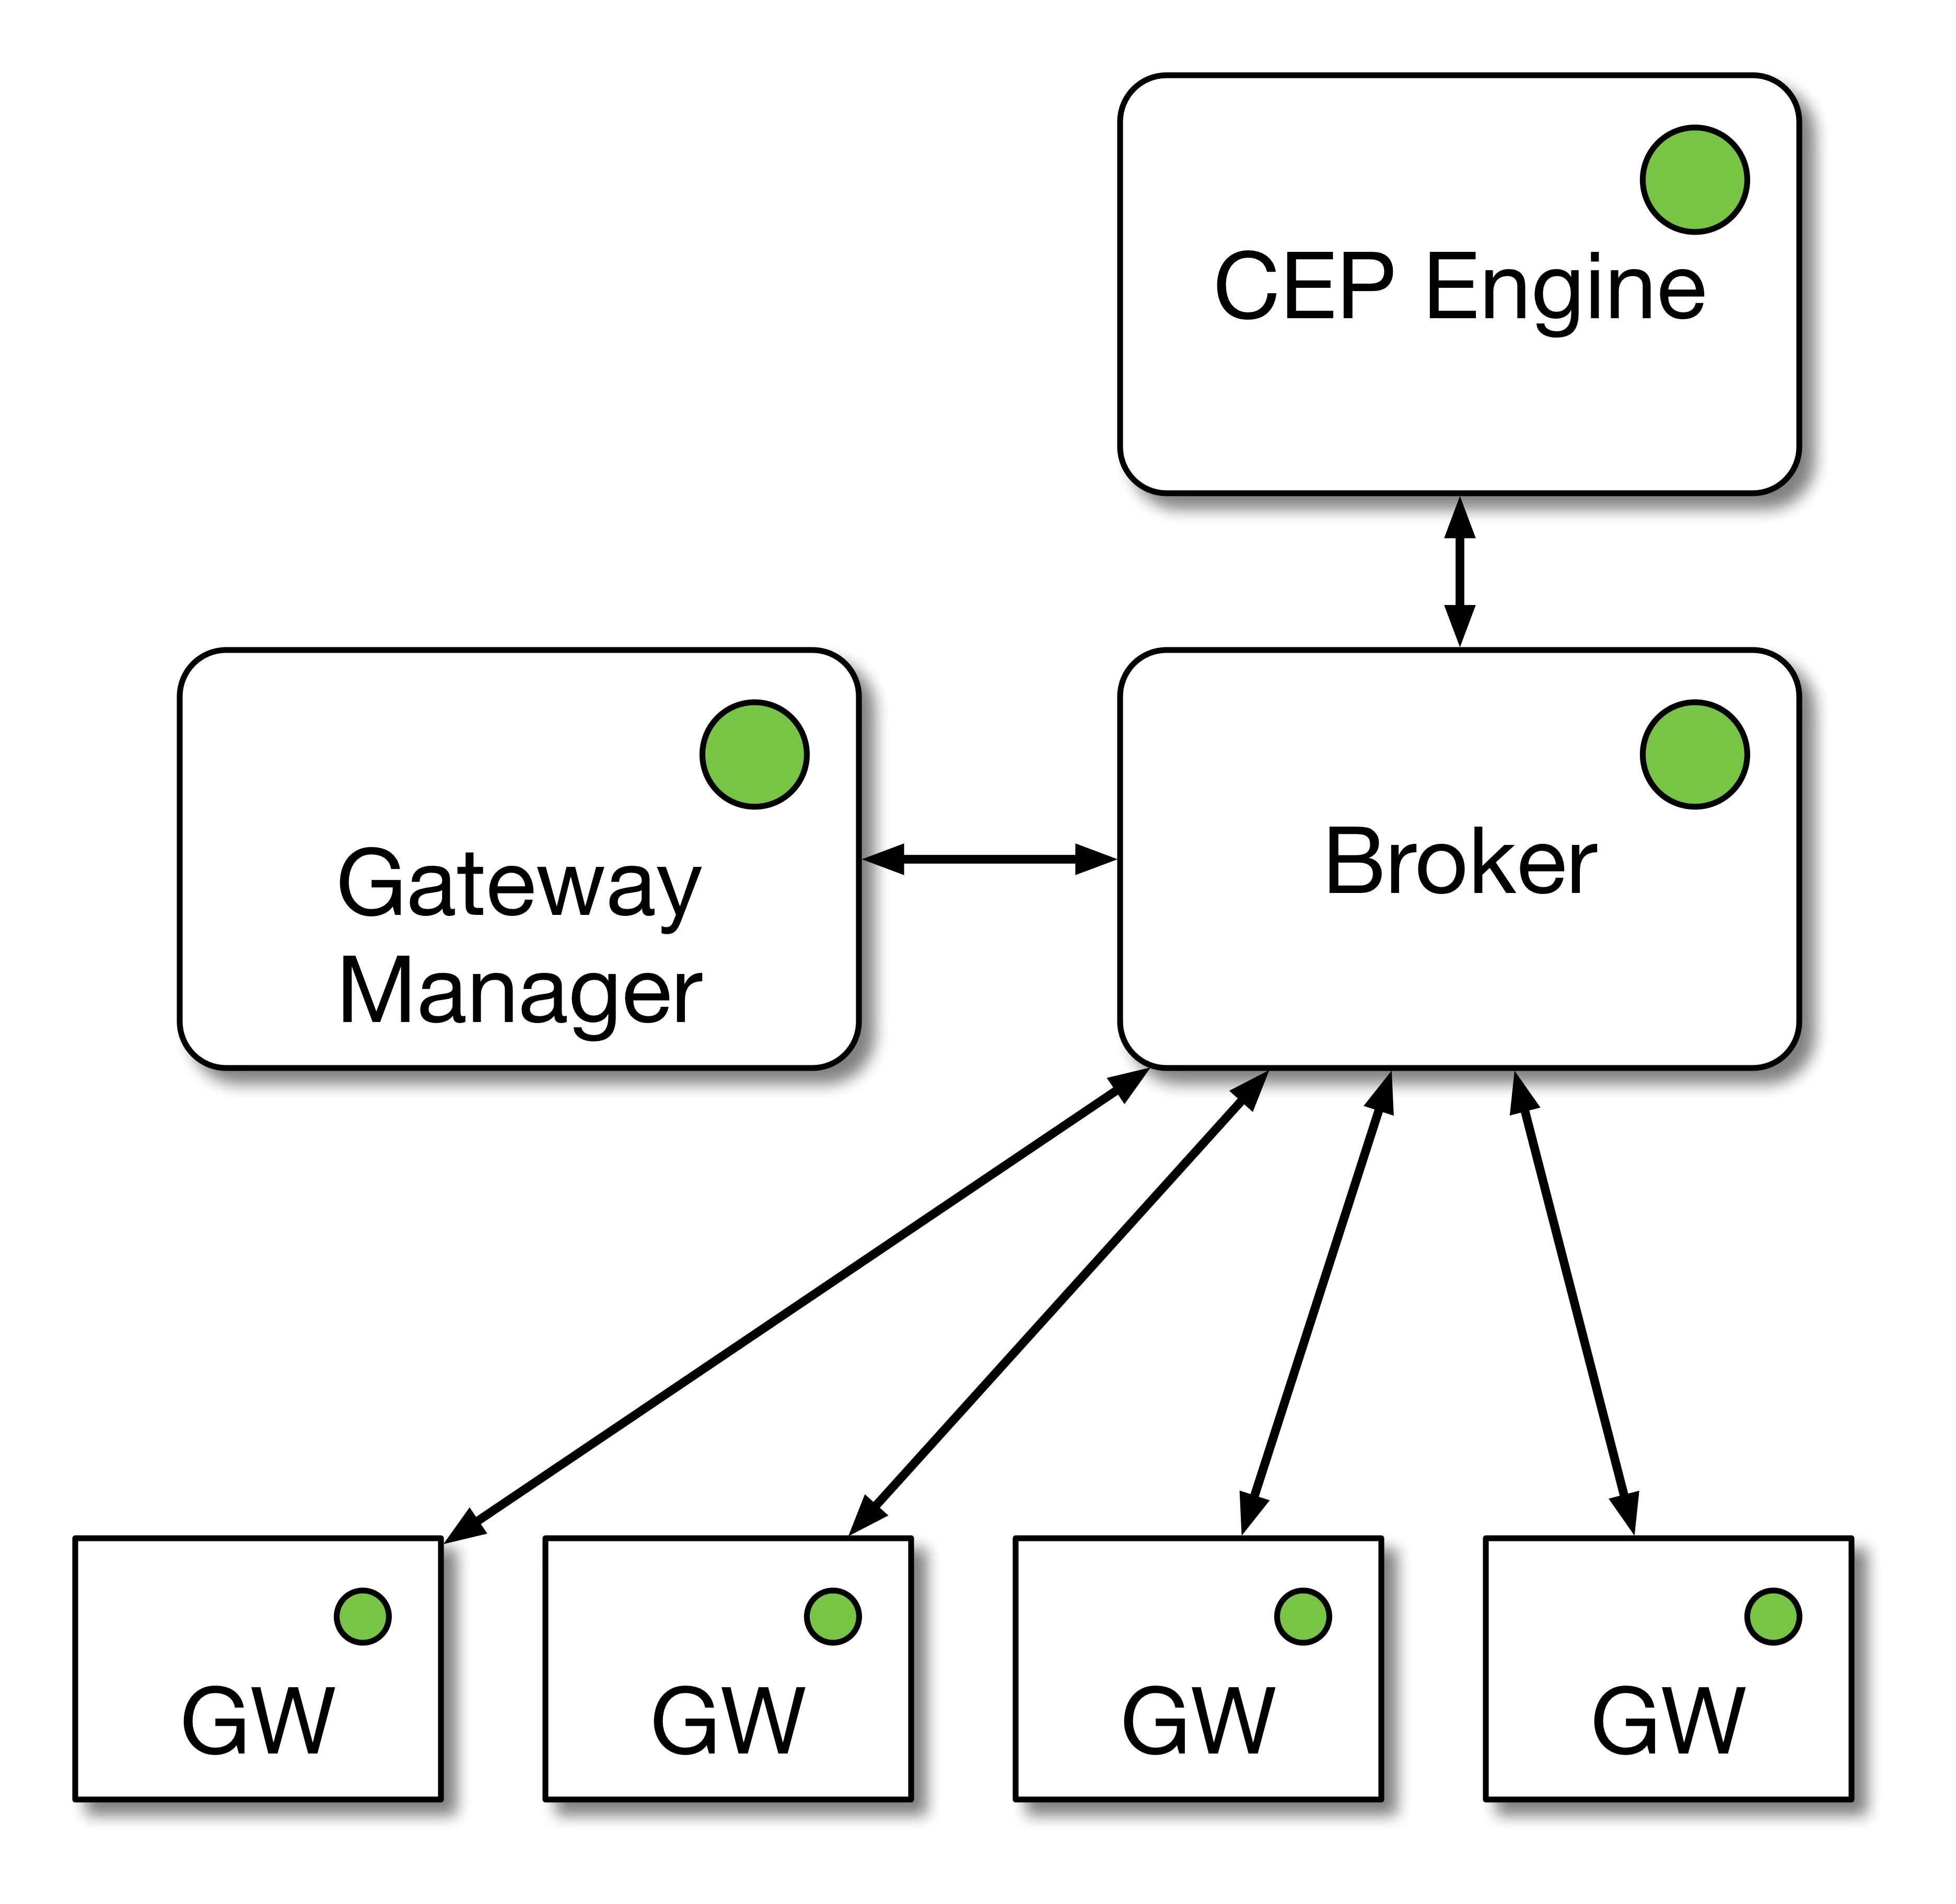
\includegraphics[width=0.4\textwidth]{figures/fs1.png}
	\caption{Functioning scenario 1.}
	\label{fig:fs1}
\end{figure}

In scenario 1, as can be observed in Figure \ref{fig:fs1}, all components are working in the expected way. Devices send events to the connected gateways, which fowards them to the central \ac{mqtt} Broker. Then the \ac{cep} Engine process them, based on the deployed rules and publishes the output events on the \ac{mqtt} Broker. Since gateways, as seen before, subscribe to all the topics that concern their devices, they receive the actions and send them to the devices.

In this scenario, the automation engine of the gateways is disabled, since the central \ac{cep} is operational. Finally, this scenario support Gateways failure, since the Gateway Manager is also operational, as it was explained in Figure \ref{fig:gwdown}.

\end{Paragraph}

\begin{Paragraph}{Scenario 2 - \ac{cep} Engine failure}
\begin{figure}[H]
	\centering
	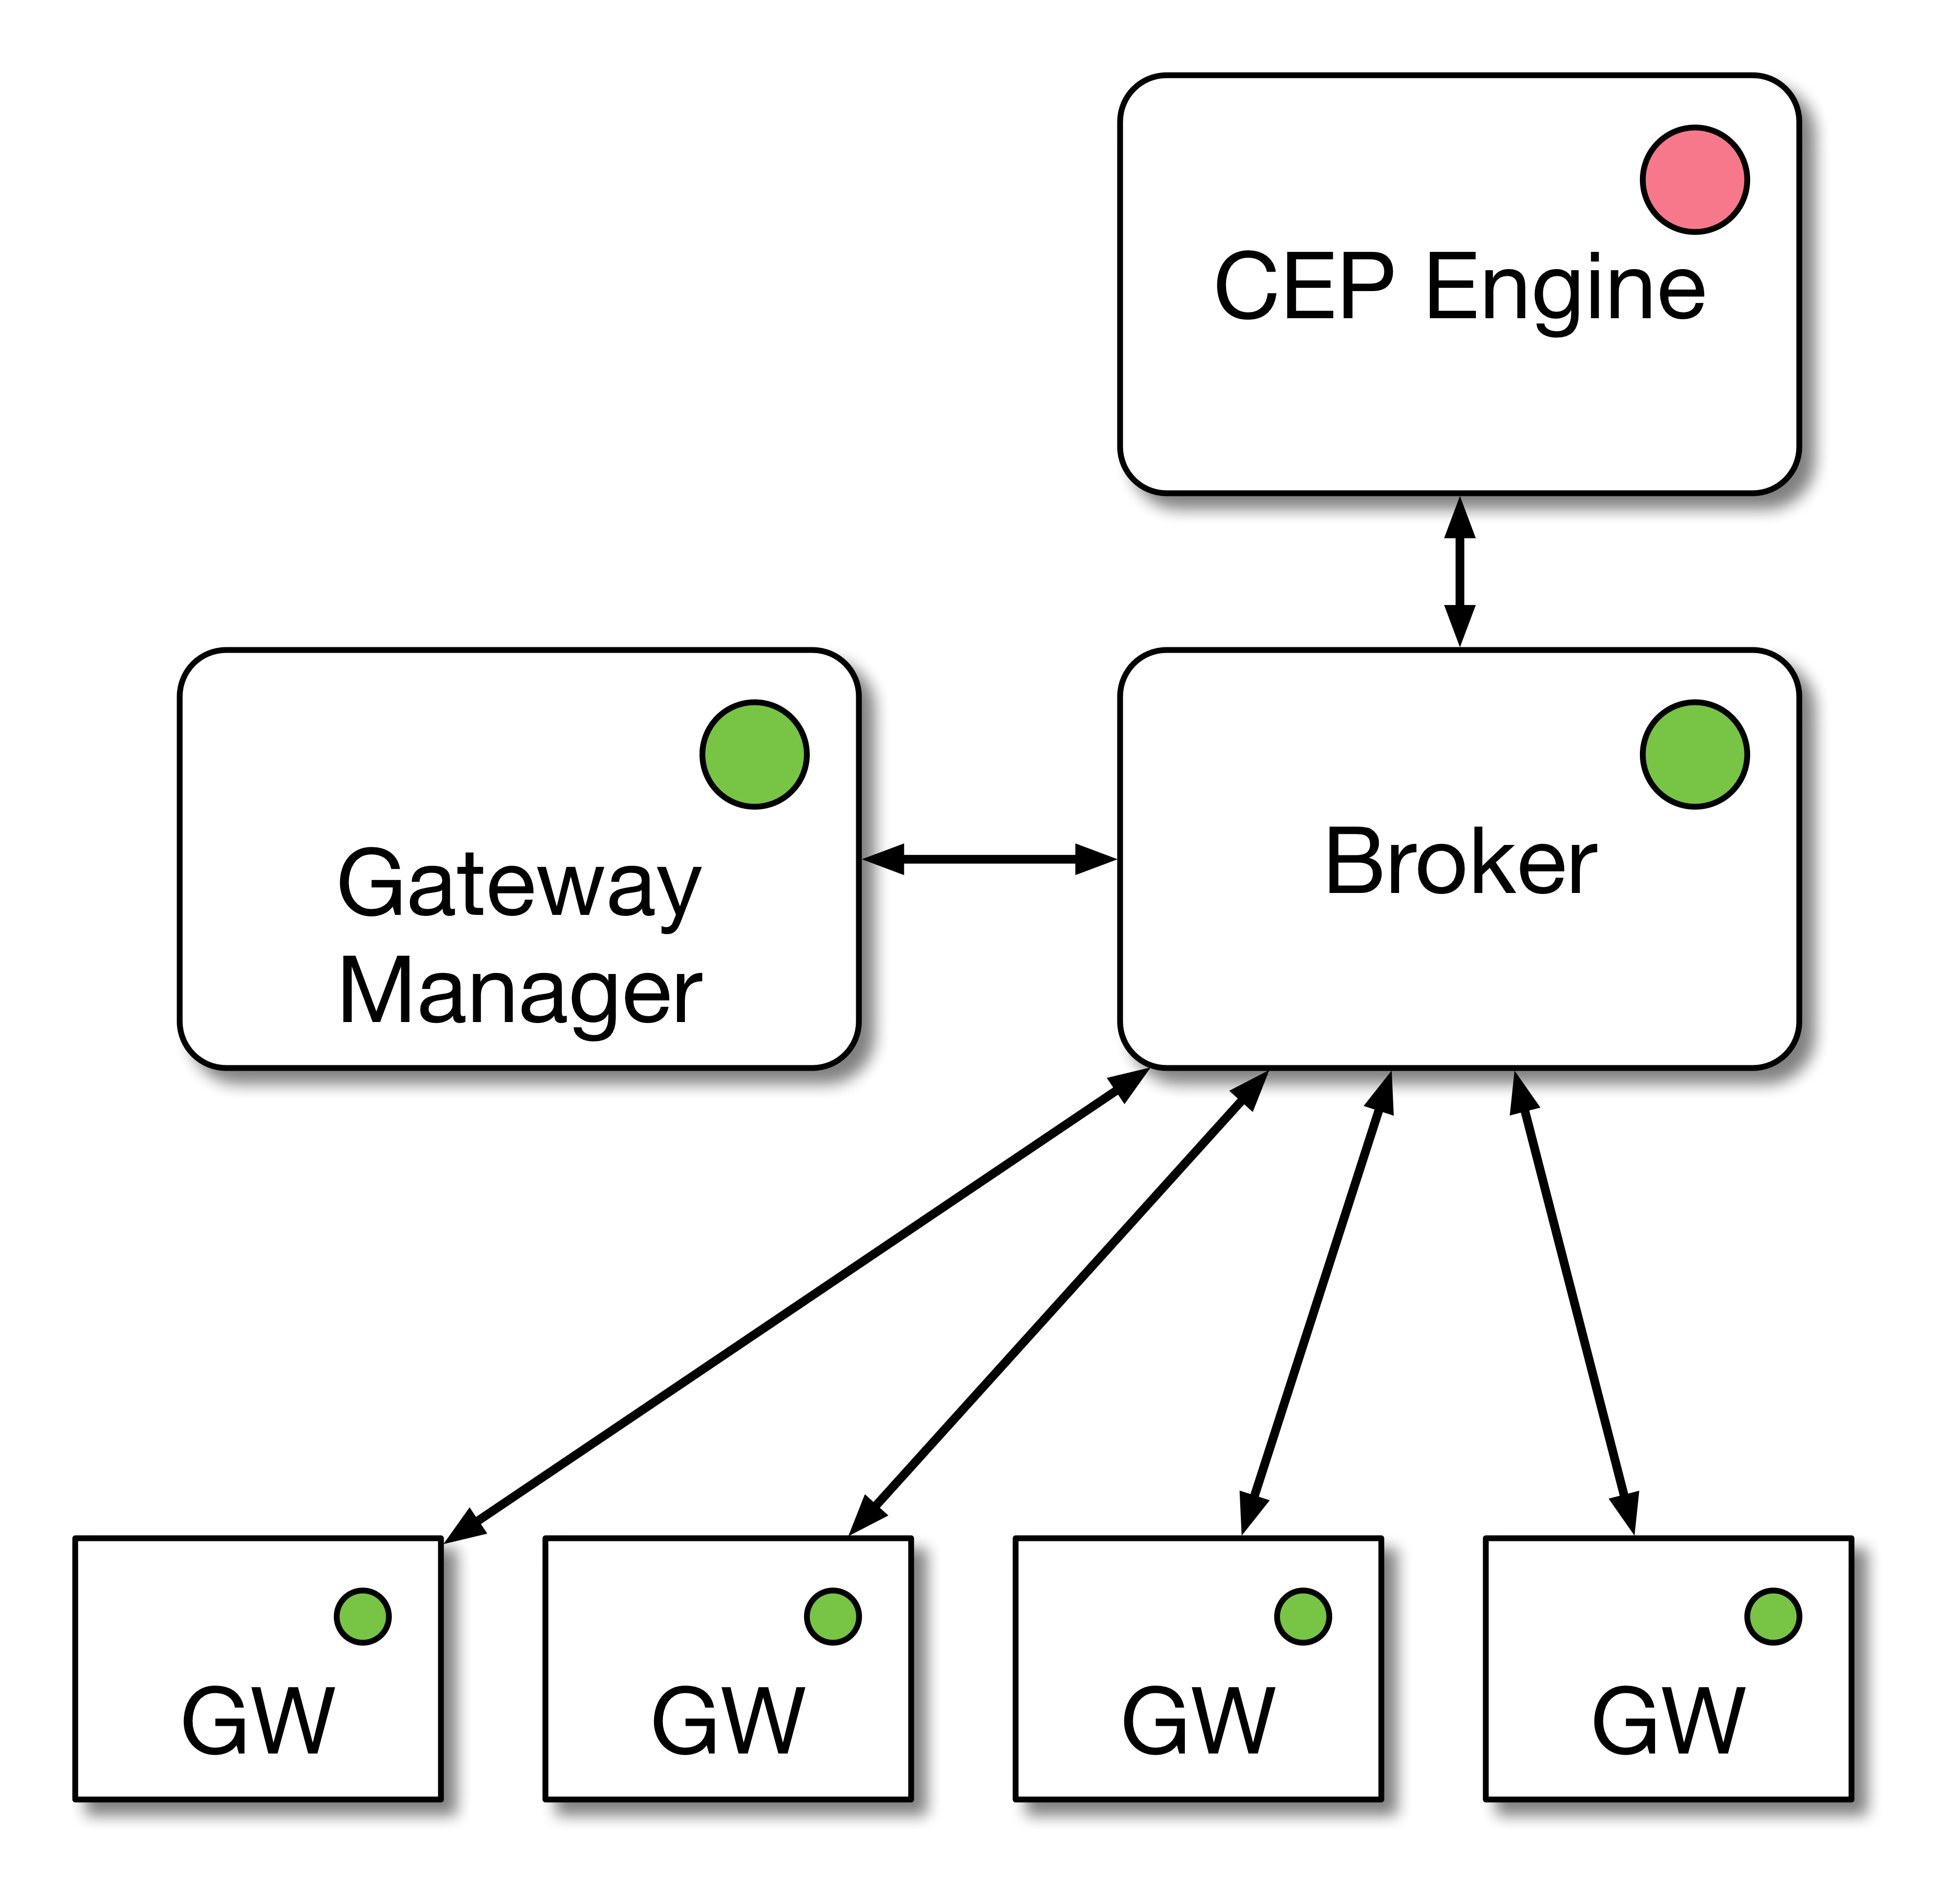
\includegraphics[width=0.4\textwidth]{figures/fs2.png}
	\caption{Functioning scenario 2.}
	\label{fig:fs2}
\end{figure}

In scenario 2, represented in Figure \ref{fig:fs2}, the \ac{cep} Engine is down. As addressed earlier, when this happens, both the Gateways and the Gateway Manager stop receiving its heart beats, and after a configurable timeout (15 seconds in this implementation), gateways subscribe, in the central broker, to the MQTT topics of the listeners present in the rules deployed by each one, and start processing device events. This process is represented in the interaction diagram present in Figure \ref{fig:gae}

\begin{figure}[H]
	\centering
	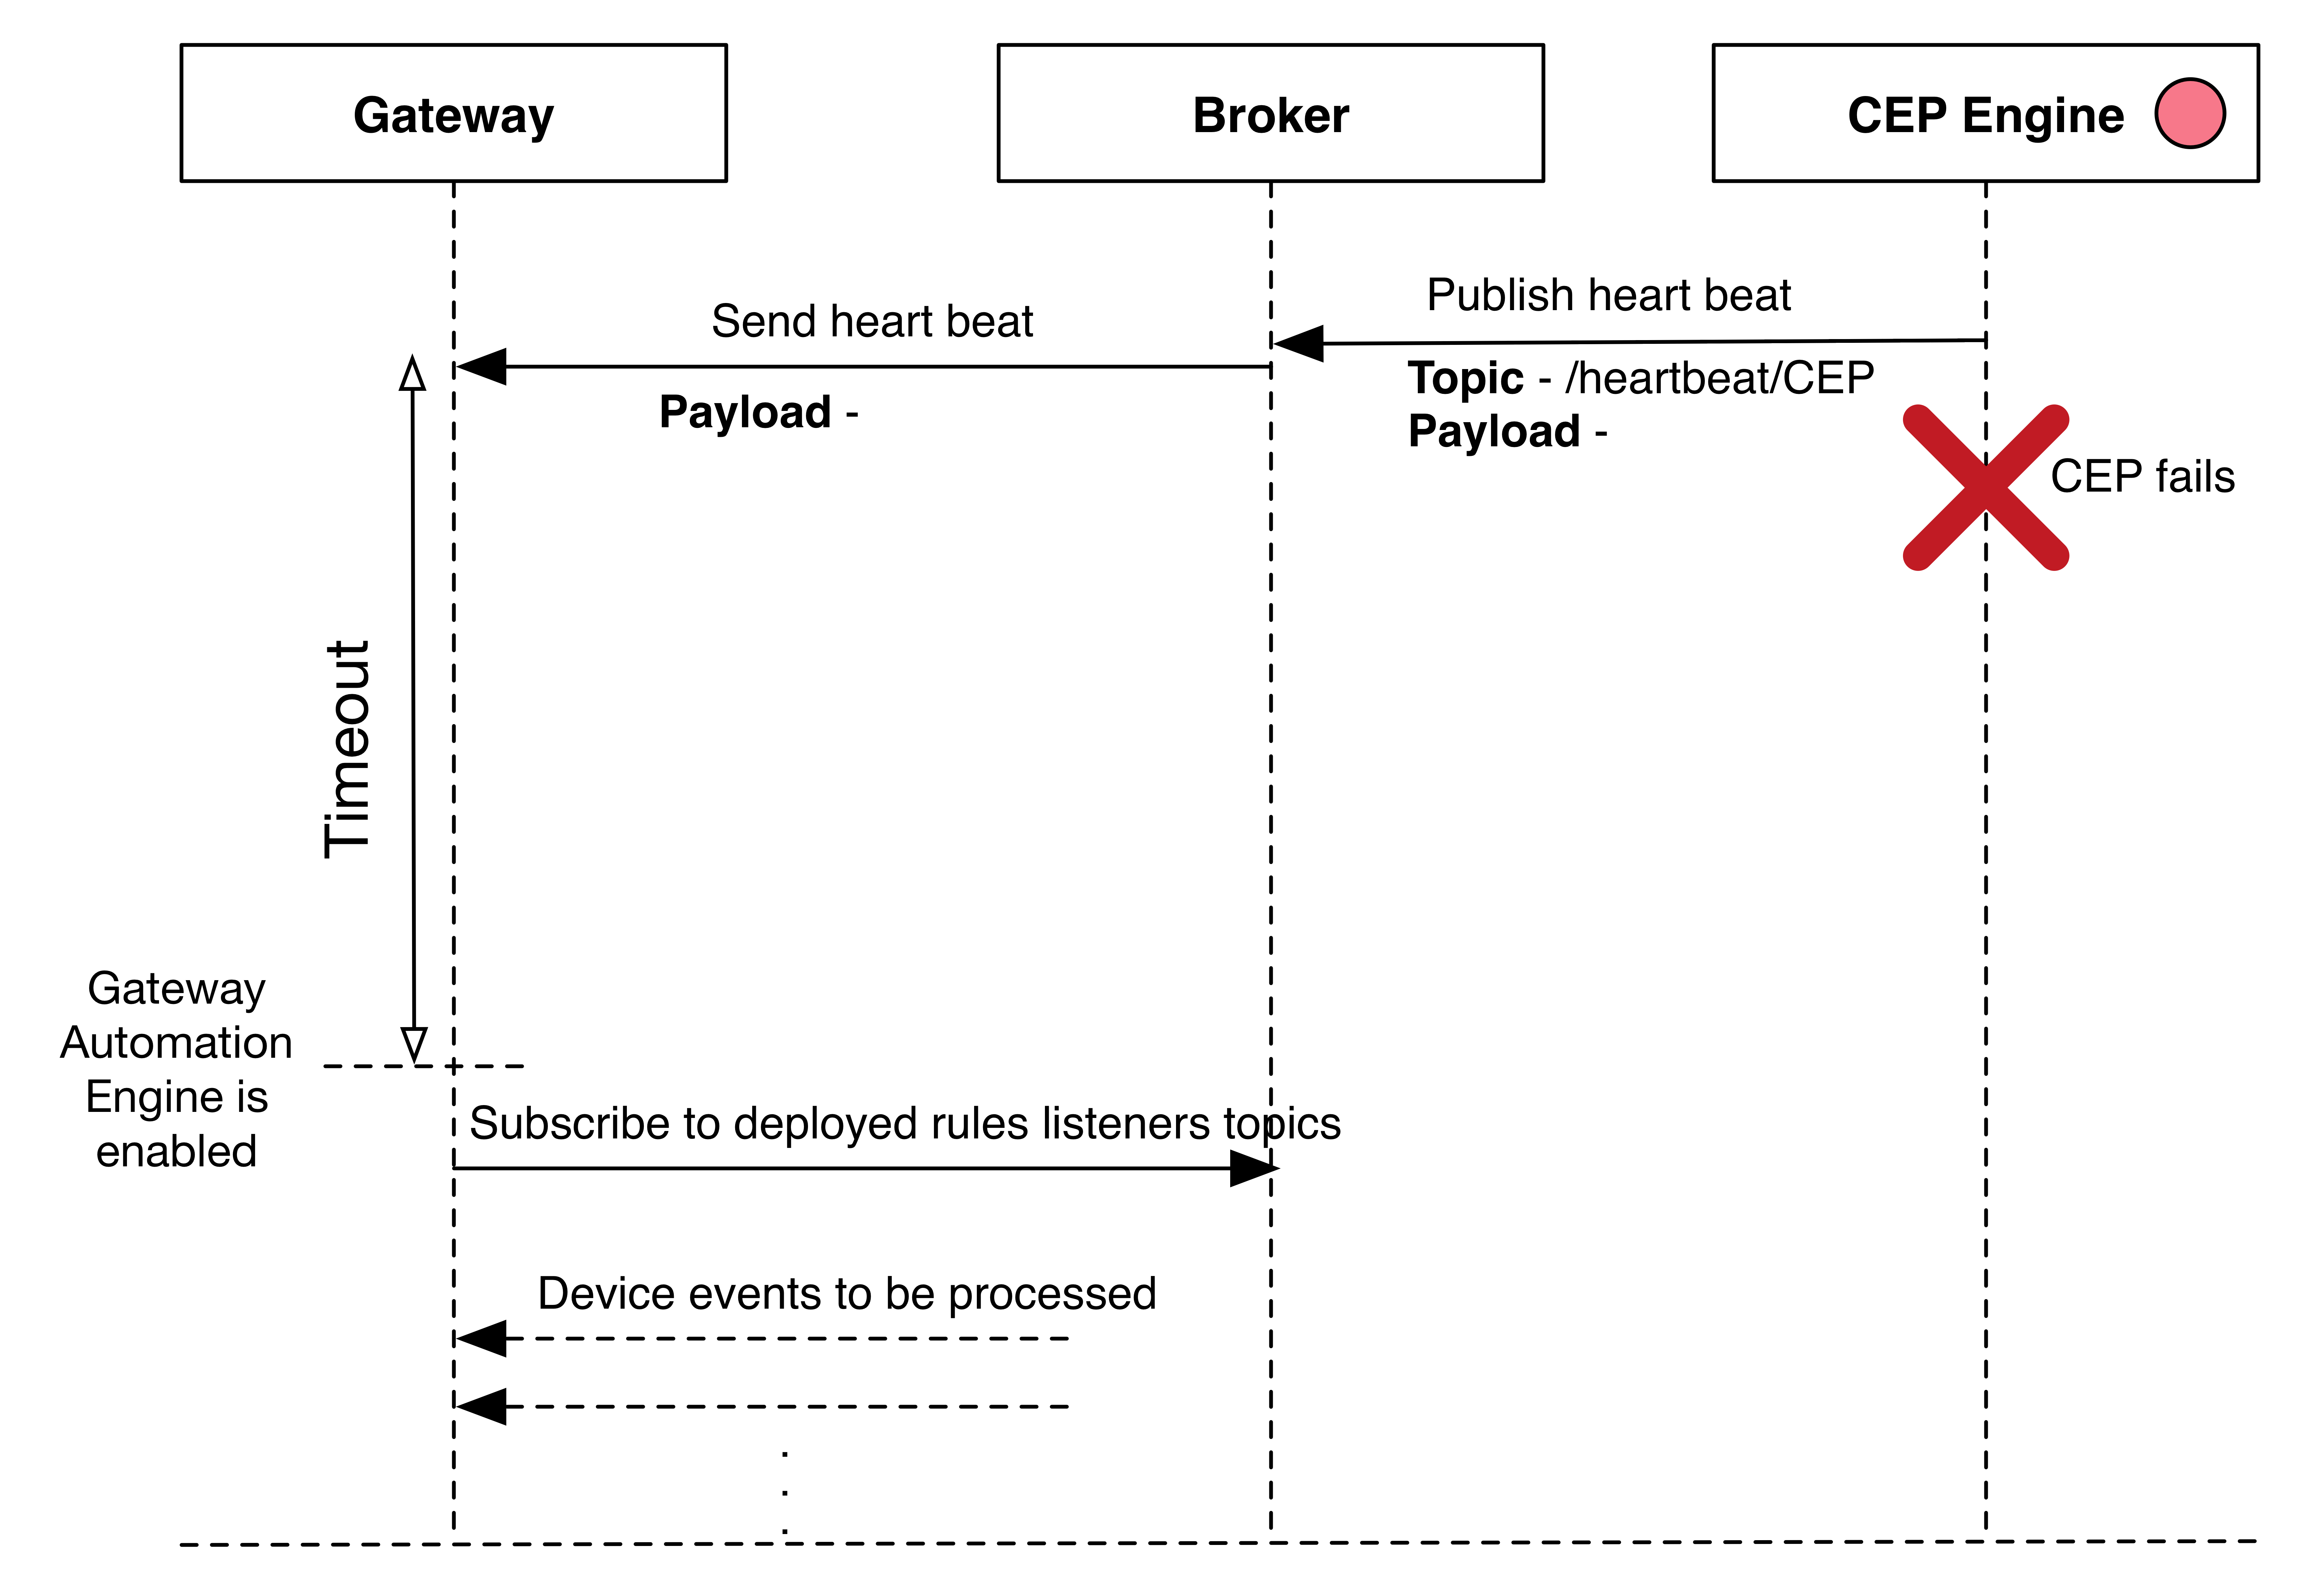
\includegraphics[width=0.8\textwidth]{figures/gae.png}
	\caption{Interaction diagram of the processes that take place when \ac{cep} Engine fails.}
	\label{fig:gae}
\end{figure}

Again, this scenario supports failures in gateways, since the Gateway Manager is operational, using the process explained earlier and represented in Figure \ref{fig:gwdown}.

\end{Paragraph}

\begin{Paragraph}{Scenario 3 - Gateway Manager failure}
	\begin{figure}[H]
		\centering
		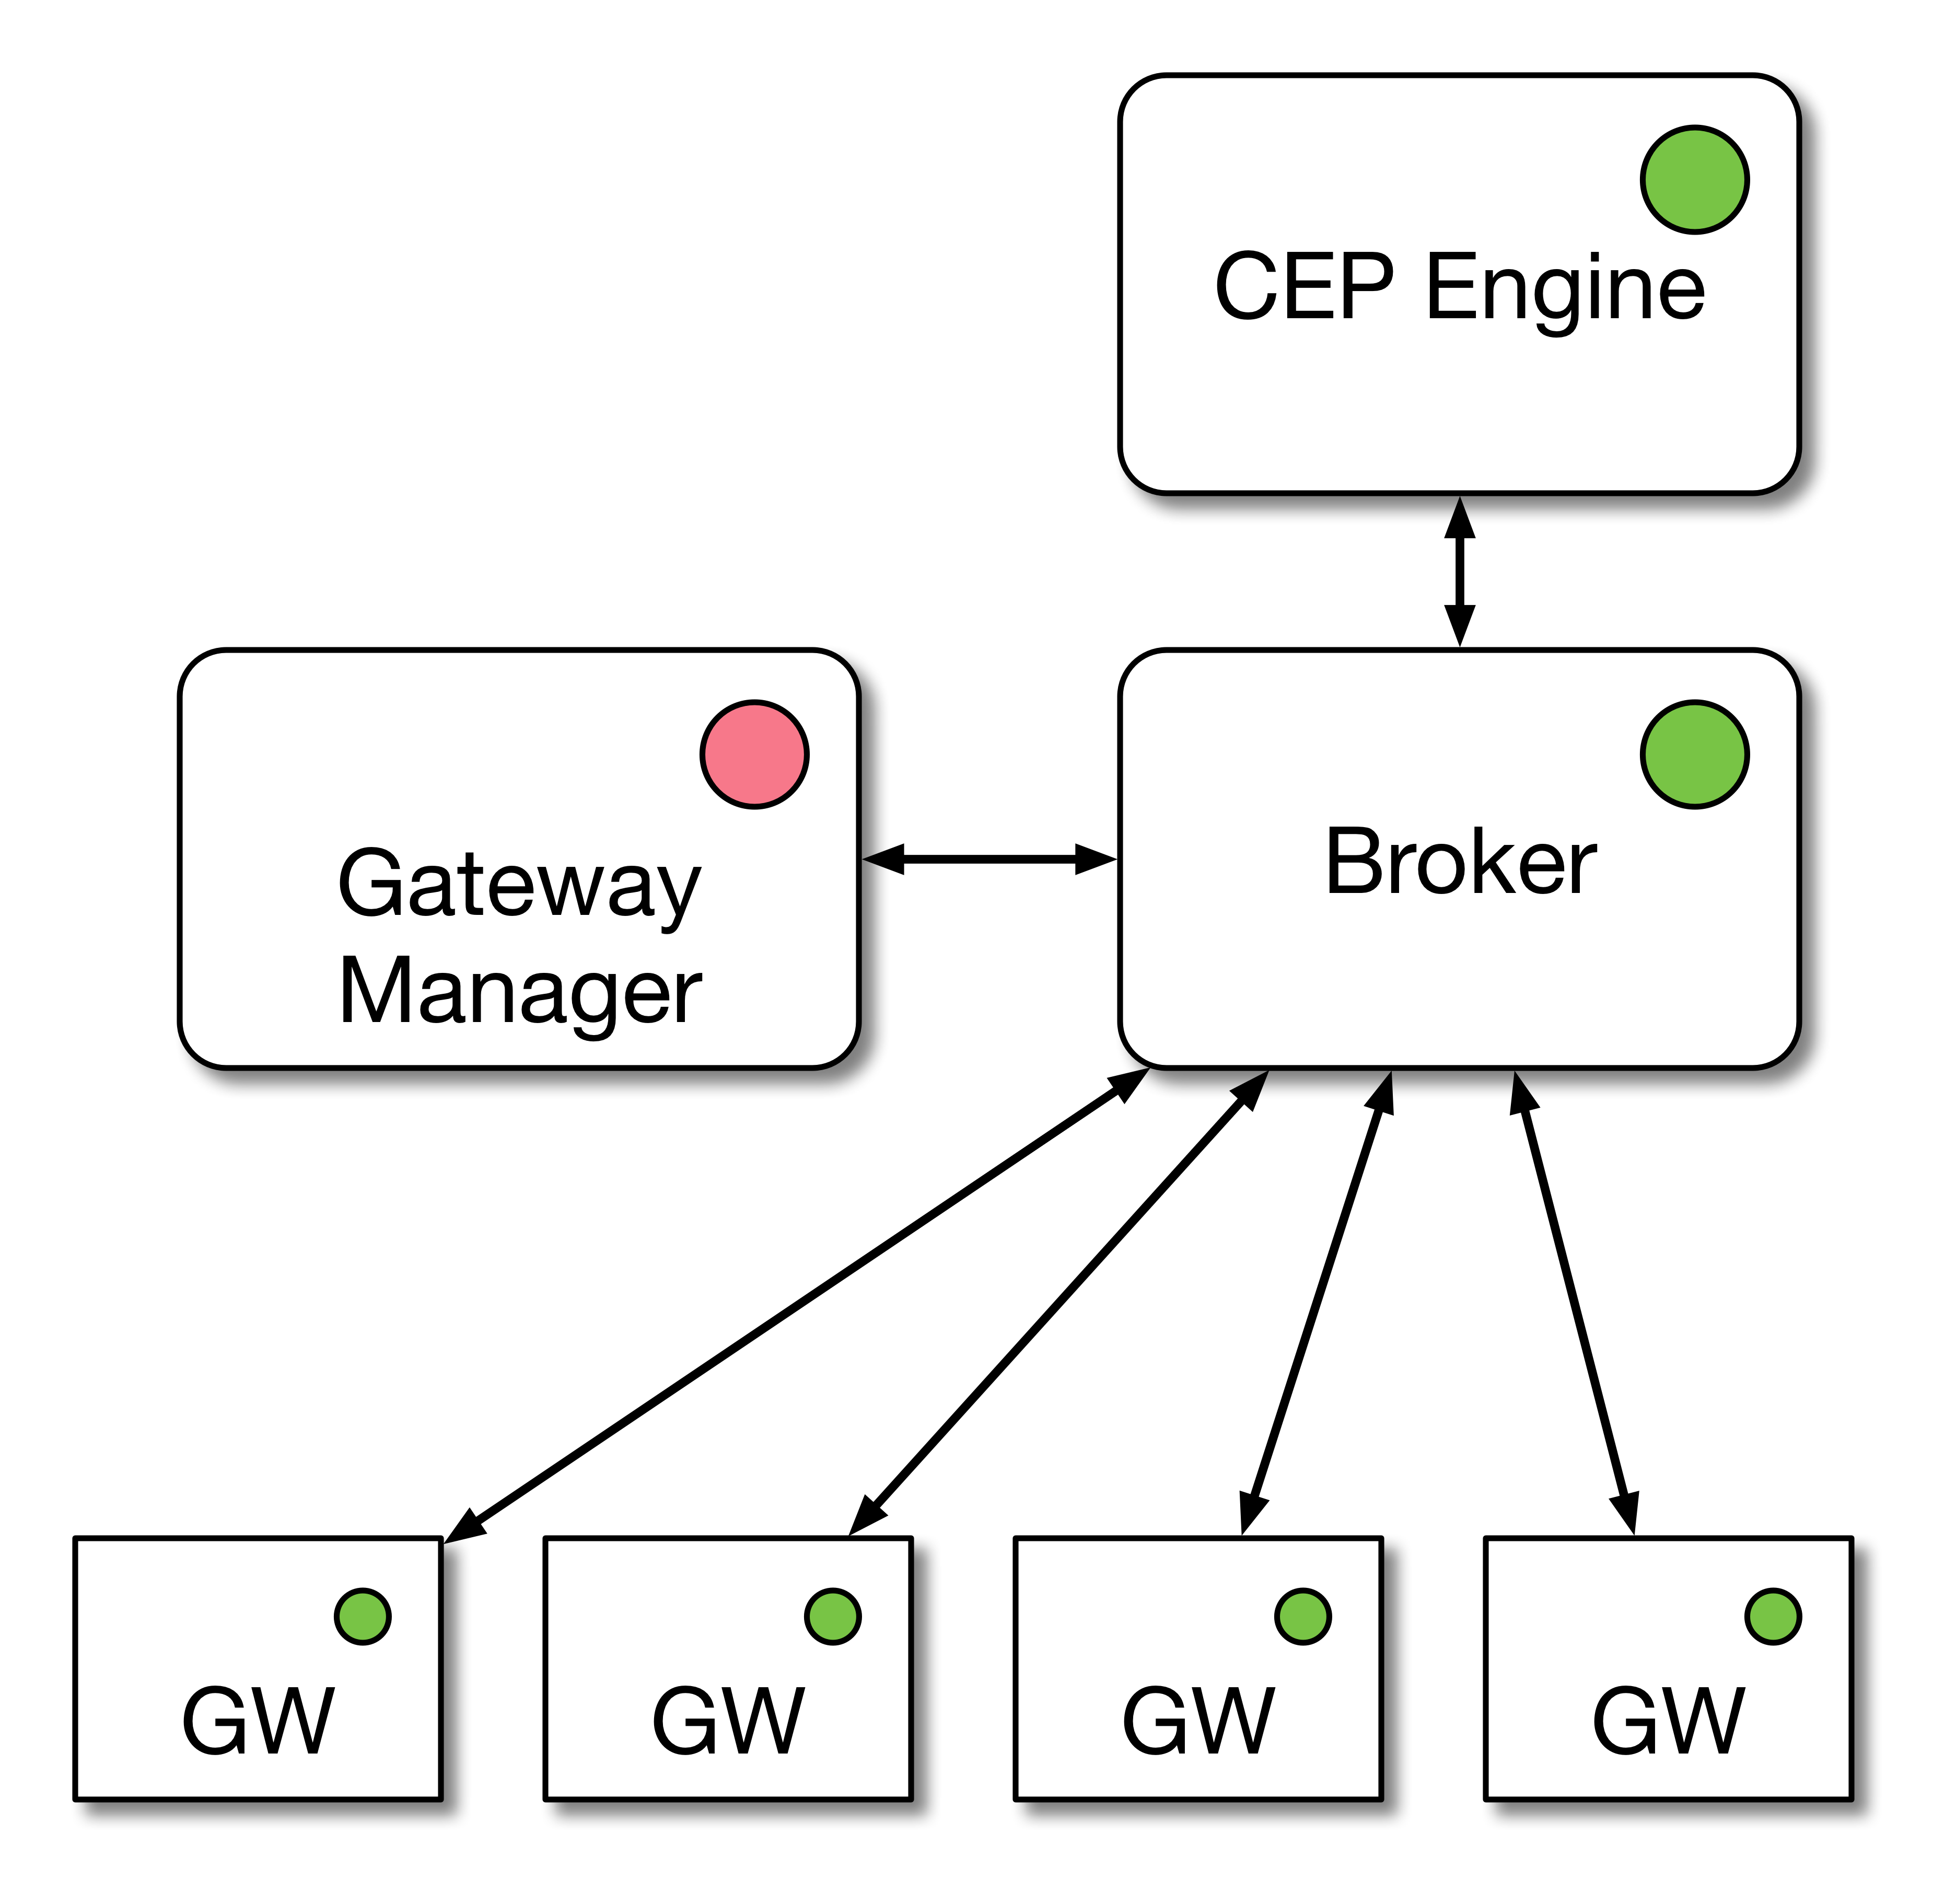
\includegraphics[width=0.4\textwidth]{figures/fs5.png}
		\caption{Functioning scenario 3.}
		\label{fig:fs5}
	\end{figure}

Scenario 3 represents a failure in the Gateway Manager while all the other components are working correctly. When this happens, the system continues to work correctly, however if a gateway fails while in this scenario, the lost devices and rules will not redistributed to other gateways and thus, the automation of some building areas will stop working. Also, while in this state, no new rules can be added to gateways. Since none of the other components are directly dependent of the Gateway Manager, for its normal functioning, its absence will not interfere with the system, and thus, the rest of the nodes can be agnostic about the Gateway Manager state.


\end{Paragraph}



\begin{Paragraph}{Scenario 4 - Gateway Manager and \ac{cep} Engine failure}
\begin{figure}[H]
	\centering
	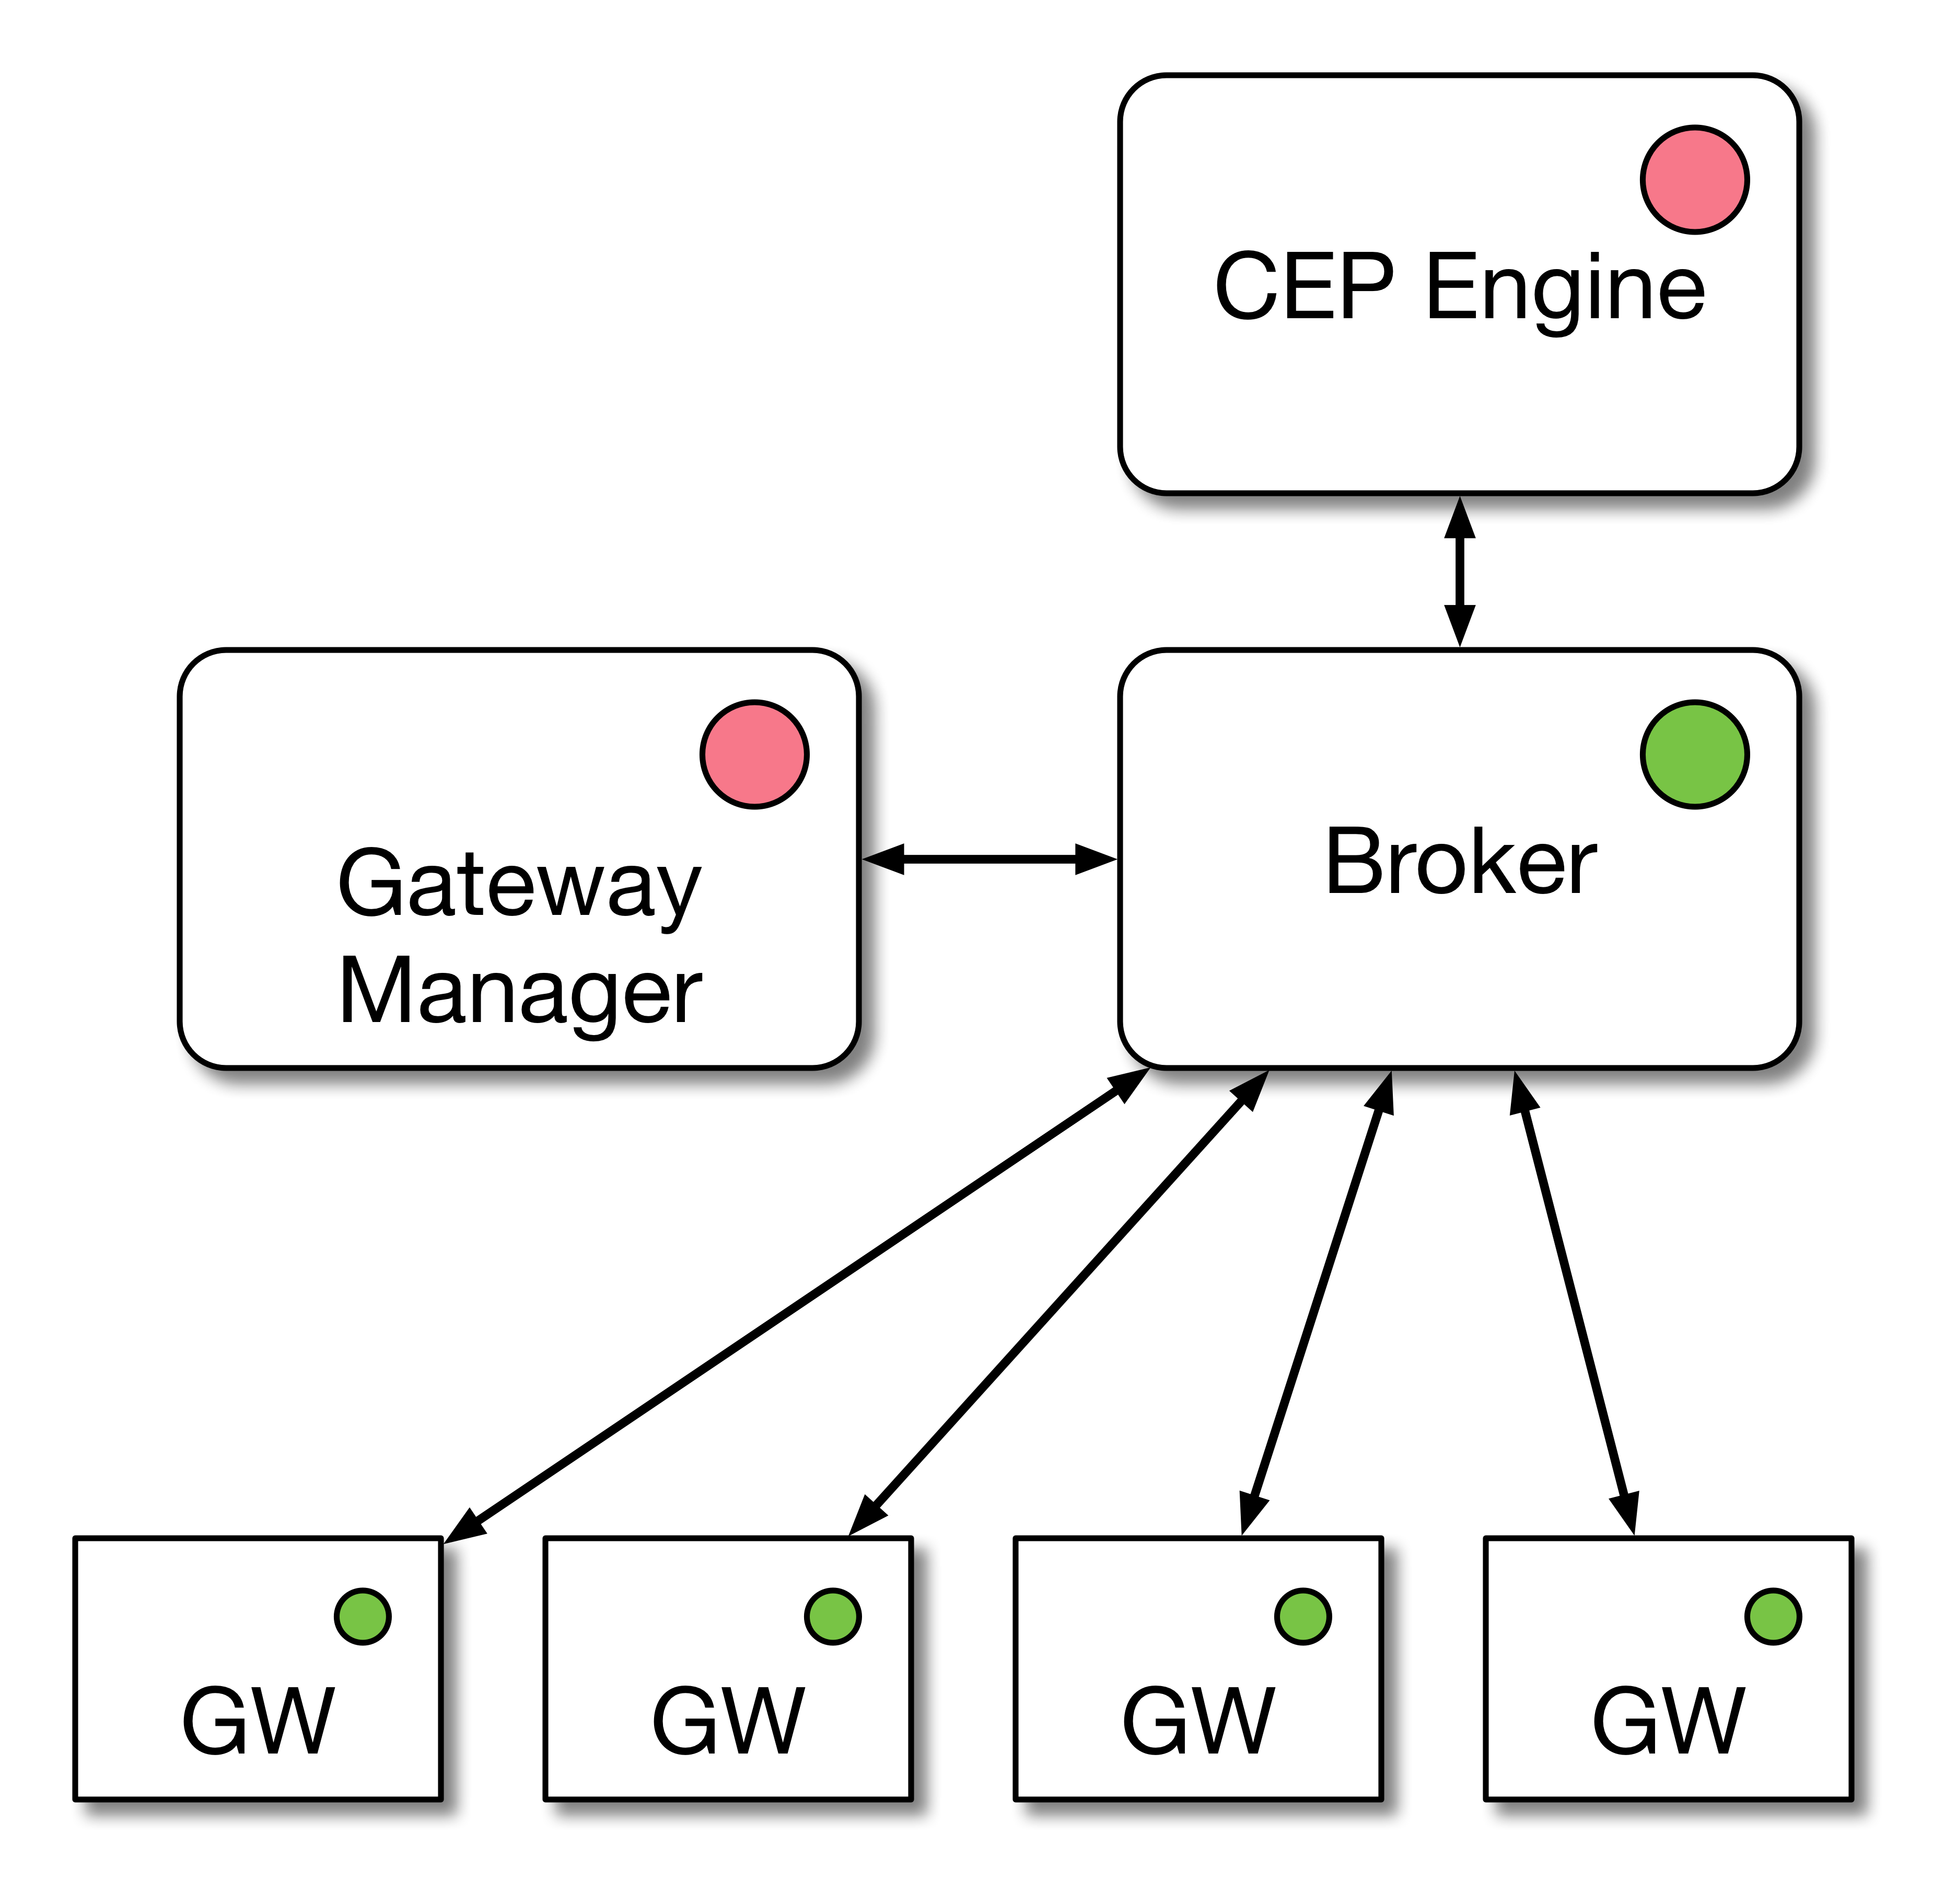
\includegraphics[width=0.4\textwidth]{figures/fs4.png}
	\caption{Functioning scenario 4.}
	\label{fig:fs4}
\end{figure}

In this scenario, both the Gateway Manager and the \ac{cep} Engine are down. This scenario is detected and produces the same alterations in the system as seen both in scenario 2, as the \ac{cep} Engine failure enables the processing of events in the gateways automation engine, and in scenario 3, as the Gateway Manager failure will disable gateways fail handling and rules distribution.



\end{Paragraph}


\begin{Paragraph}{Scenario 5 - \ac{mqtt} Broker failure}
	\begin{figure}[H]
		\centering
		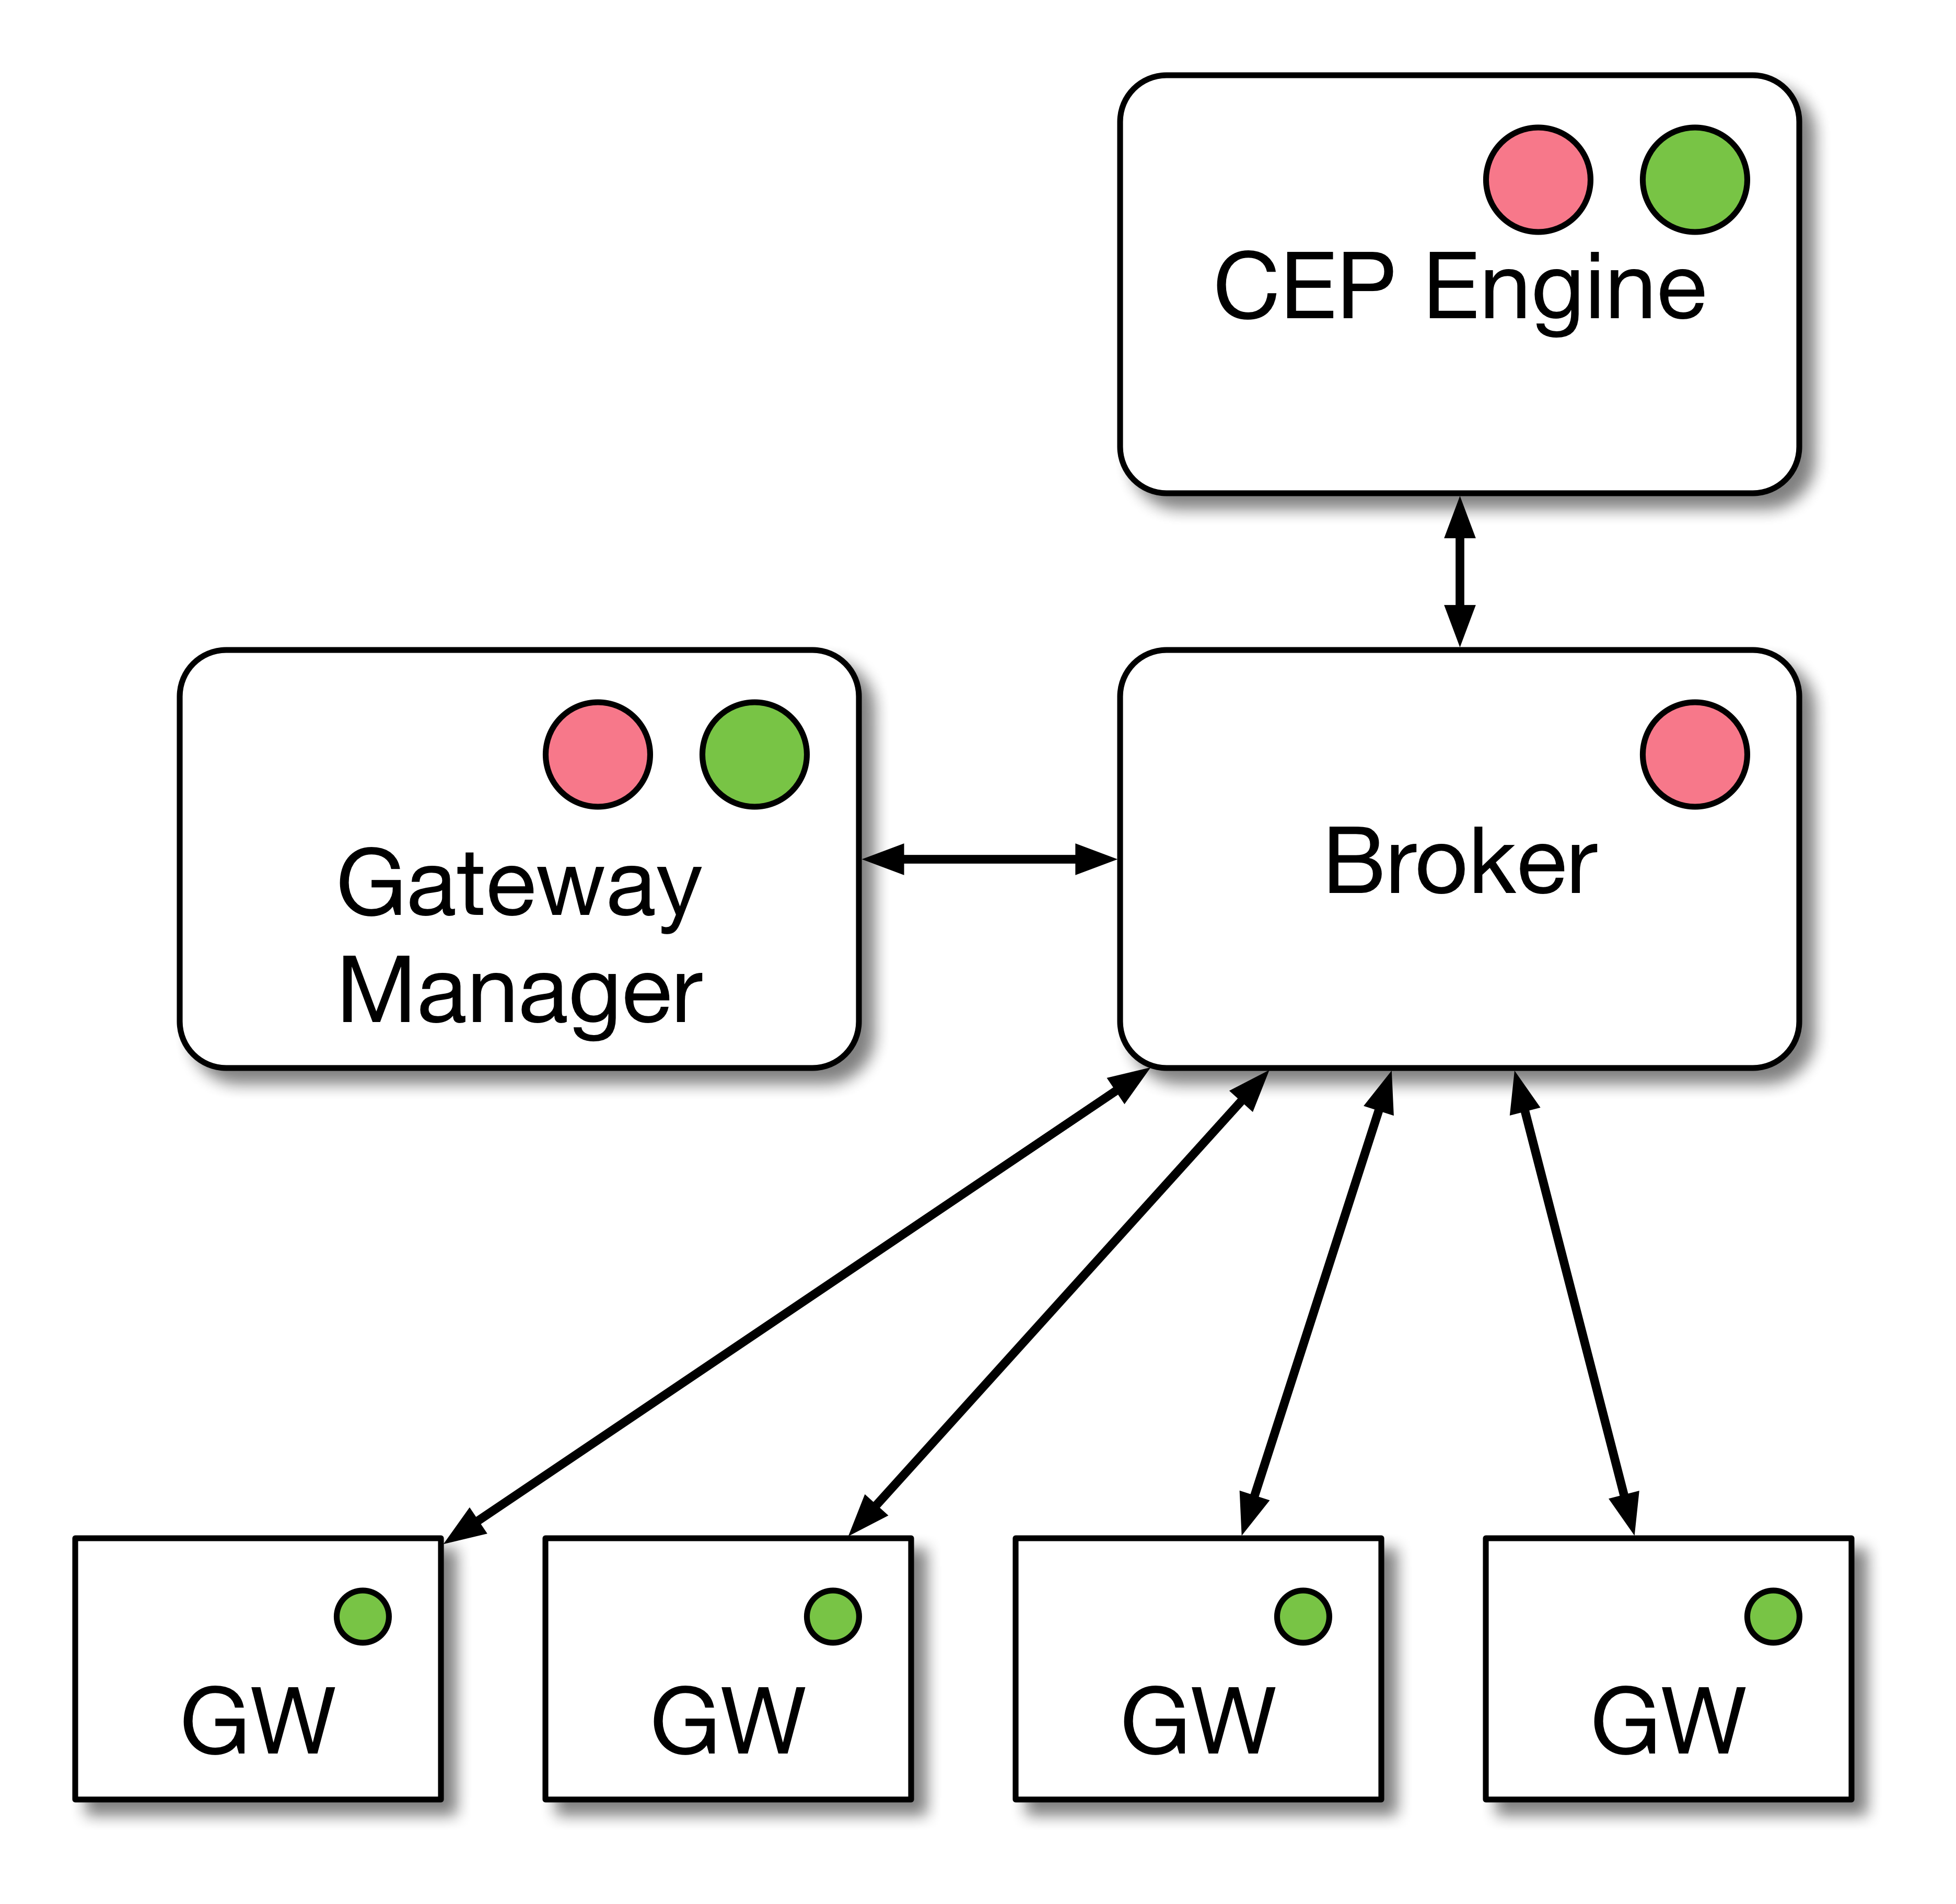
\includegraphics[width=0.4\textwidth]{figures/fs3.png}
		\caption{Functioning scenario 5.}
		\label{fig:fs3}
	\end{figure}

This last scenario is the most severe and complex one, since if the central \ac{mqtt} broker is down, the communication between gateways and the other components (\ac{gm} and \ac{cep} Engine) is interrupted. When gateways are aware that the central broker is down, the automation engine is enabled, and the events generated by the devices, are sent directly to the brokers of gateways that have rules that process those events. Also, when a gateway receives an event to be processed, it sends the resulting event to gateways that have devices triggered by that event. As seen before, the Gateway Manager synchronizes, between all gateways, the information needed to implement these features: each gateway knows exactly to which gateways the events, of each device it controls, should be sent to be processed, and also, has the information of to which gateways should the processed events be sent. While in this scenario, which could be triggered by a whole building network failure, the gateways would still be able to connect through bluetooth with devices, and thus, the building's most core functionalities, such as lighting, will still be able to work. 

\end{Paragraph}

\begin{Paragraph}{Summary}

	
Looking at the described scenarios, it is noticeable a degradation over the system functionalities. However, regardless the scenario, the most important automation features, that are crucial to the system, can be safeguarded by deploying emergency rules in gateways. Even when core components of the system are down, gateways can still ensure a minimum functionality to the building by themselves. Bellow in Table \ref{summary}, are specified the scenarios, and the component's state and distinctive features present in each one of them.

	
\begin{table}[H]
	\centering
	
		\resizebox{\textwidth}{!}{\begin{tabular}{|c|c|c|c?c|c|c|}
		\hline
		\textbf{Scenarios} & \textbf{Broker} & \textbf{CEP Engine} & \textbf{\begin{tabular}[c]{@{}c@{}}Gateway \\ Manager\end{tabular}} & \textit{\textbf{\begin{tabular}[c]{@{}c@{}}Gw Failure\\ Handling\end{tabular}}} & \textit{\textbf{\begin{tabular}[c]{@{}c@{}}Gw Automation \\ Engine Enabled\end{tabular}}} & \textit{\textbf{\begin{tabular}[c]{@{}c@{}}Gw-Gw \\ Communication\end{tabular}}} \\ \hline
		\textbf{1}         & Up              & Up                  & Up                                                                  & Yes                                                                                  & No                                                                                             & No                                                                               \\ \hline
		\textbf{2}         & Up              & Down                & Up                                                                  & Yes                                                                                  & Yes                                                                                            & No                                                                               \\ \hline
		\textbf{3}         & Up              & Up                  & Down                                                                & No                                                                                   & No                                                                                             & No                                                                               \\ \hline
		\textbf{4}         & Up              & Down                & Down                                                                & No                                                                                   & Yes                                                                                            & No                                                                               \\ \hline
		\textbf{5}         & Down            & N/A                 & N/A                                                                 & No                                                                                   & Yes                                                                                            & Yes                                                                              \\ \hline
	\end{tabular}}
\caption{Scenarios summary table.}
\label{summary}
\end{table}


As can be observed, the gateway's Automation Engine is only enabled either on scenarios where the \ac{cep} Engine is down, or when the broker is unavailable, since it connects gateways to the \ac{cep} Engine. Also, since the Gateway Manager is the component responsible for handling gateway failures as redistribute devices and rules, when this component is down, the gateway's failure handling is not assured. Finally, in scenario 5, since the central broker is down, gateways need to communicate directly with each others in order to insure the processing of its events.

As referred before, the system should be working on scenario 1 the great majority of time, however, since all the other scenarios ensure a basic functionality to the system, a fail in a component would not impose great consequences to the system. Therefore, the implemented features addressed all the requirements and objectives for the proposed dissertation. 

\end{Paragraph}


	\chapter{Evaluation and Results}
\label{chapter:evaluation_and_results}



In chapter 4, it was presented the implementation of the proposed solution, giving a description of all the implemented features and how the system should adapt and react in different scenarios, in order to maintain, at least, a minimum functionality, always.

The objective for this chapter is to validate the proposed solution. Firstly, in section \ref{results:scenario}, a deployment scenario overview will be given, highlighting the devices and tools used for that purpose. Following, in section \ref{results:results}, the obtained results for different tests will be analysed. With the requirements, addressed in chapter 3, taken into consideration, the performance of the automation engine, implemented in gateways, will be evaluated, and also, to judge the capacity of the system to react to abnormal functioning scenarios, the reaction time to this occurrences will be measured.

\newpage

\section{Deployment Scenario}
\label{results:scenario}



The final deployment scenario, used to test and validate the system and illustrated in Figure \ref{fig:performance}, is composed by the Building Manager platform, the WSO2 \ac{cep} Engine, the Gateway Manager and two Gateways, all communicating through the MQTT Broker. 

The Building Manager is the component responsible for supporting the user-friendly platform to create rules and distribute devices through the building planer. This platform was hosted in a Linux virtual machine equipped with a single-core processor and 1 gigabyte of memory.

The WSO2 \ac{cep} engine, which is one of the core components of the whole system, as it is the primary processor of events, based on the logic specified in the rules. This component, required a more powerful machine than the Building Manager component , being hosted in a Linux virtual machine with a quad-core processor and 4 gigabytes of memory.

\begin{figure}[H]
	\centering
	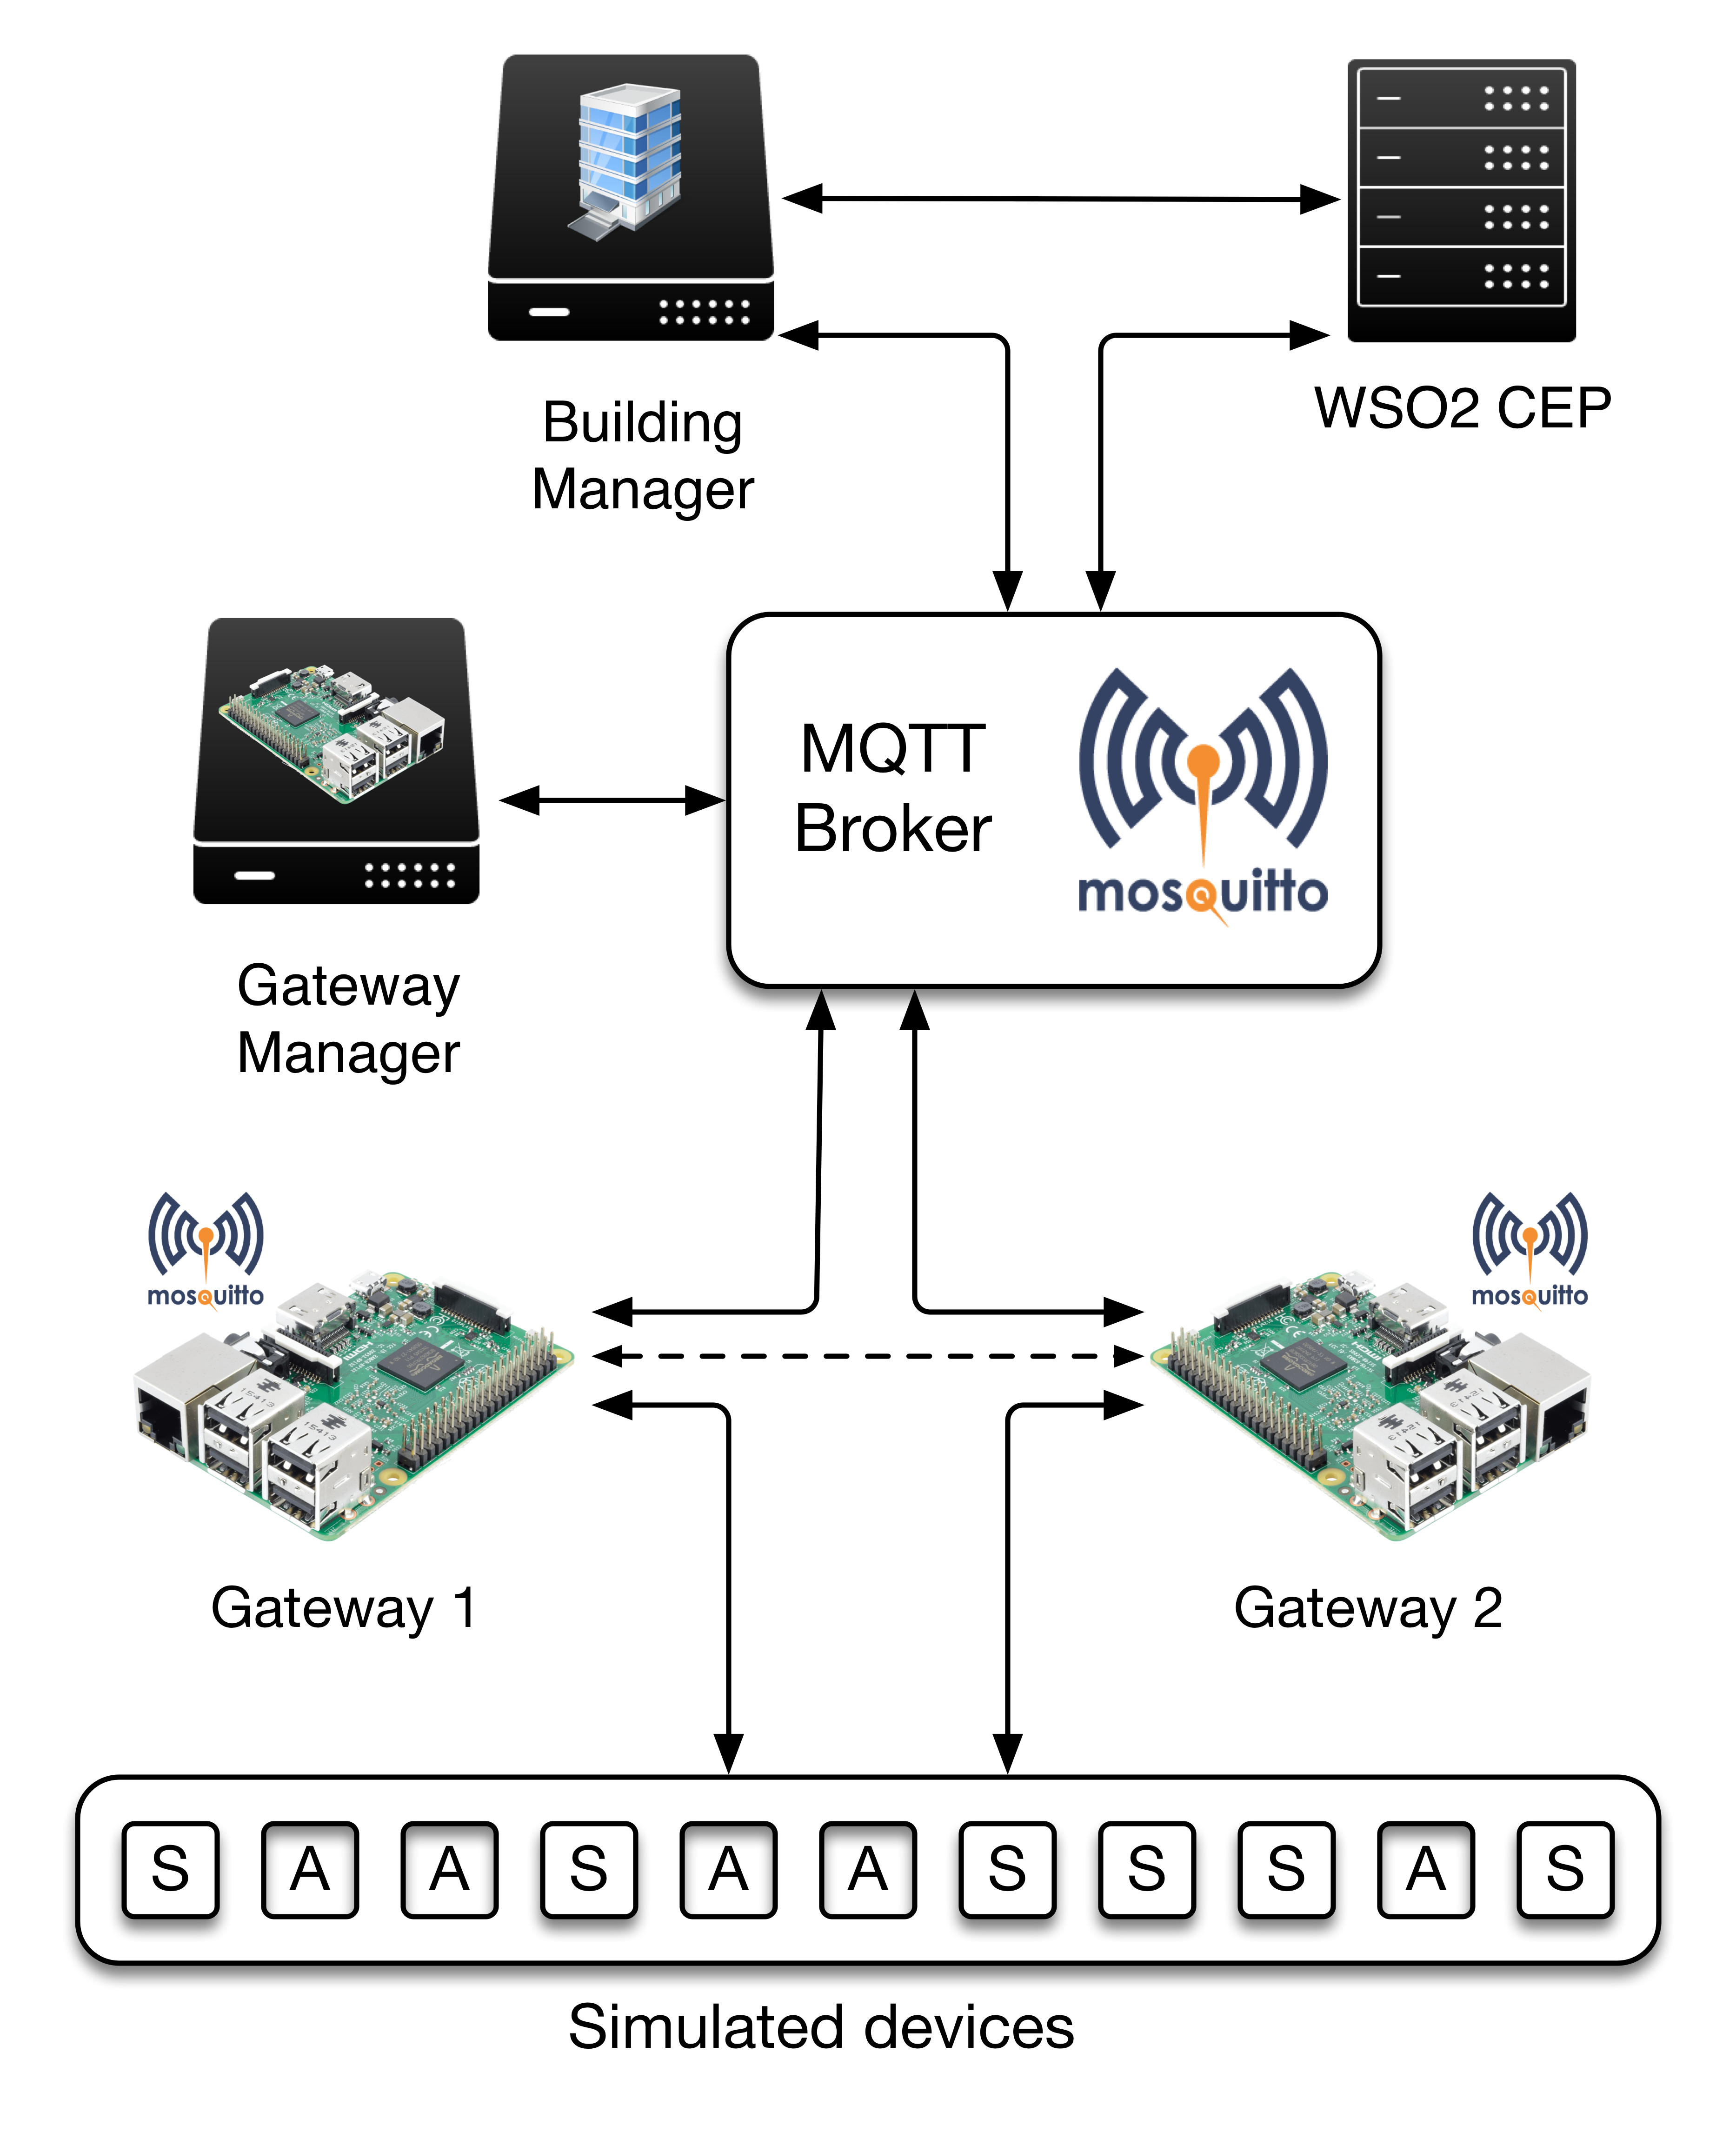
\includegraphics[width=0.7\textwidth]{figures/deployment.png}
	\caption{Deployment Scenario.}
	\label{fig:deploy}
\end{figure}

Regarding the Gateway Manager, it contains both a software for gateway's management and a web-server to offer a platform to check the state of each gateway and the general state of the system. This component was also deployed in a Linux virtual machine with a dual-core processor and 2 gigabytes of memory.

In order to assure the communication between the different components, the Mosquitto MQTT Broker was deployed in a separate virtual machine with a dual-core processor and 2 gigabytes of memory.

Finally, concerning the gateways, which are responsible for communicate with devices and, in some scenarios, process events using its Automation Engine. In this deployment scenario were used simulated devices. To further explain, a equal set of devices were configured in both gateways, simulating a scene where the devices are in range of two different gateways. Each gateway were equipped with code to generate events of the devices assigned to them, by the Gateway Manager. If a gateways had control over a sensor, it should send events with a fixed programmable frequency. This was used for the testing scenario addressed in section \ref{results:fail}%The simulated devices used were motion sensors and lights actuators and it was deployed a rule, to trigger a light on for 5 seconds, each time a motion sensor sends an event. 





\section{Performance Results}
\label{results:results}

In this section will be presented the results and discussion of the tests preformed. Firstly, in section \ref{results:cep} the latency of the gateway's Automation Engine will be mesured and then, in section \ref{results:fail}, the reaction time to system failures will be evaluated.


\subsection{Gateway's Automation Engine Performance}
\label{results:cep}

In order to evaluate the gateway's Automation Engine performance, a stress test was preformed. The objective was to measure the processing time of events, in five different stress situations: first, sending a single event and measure the time taken by the engine to produce an output response, and then increase the number of consecutive events, 10, 100, 1000 and 10000, to not only measure the time taken to process all those events, but also to check if all events were processed. 

For this test, two python scripts were made: one to send a programmable number of events consecutively, and other to measure the time since the first event was sent, and the last response action was received. The deployed rule consisted in inputting a motion event and respond with an event to turn on a light as result. The results of this test are expressed in Figure \ref{fig:performance}.

\begin{figure}[H]
	\centering
	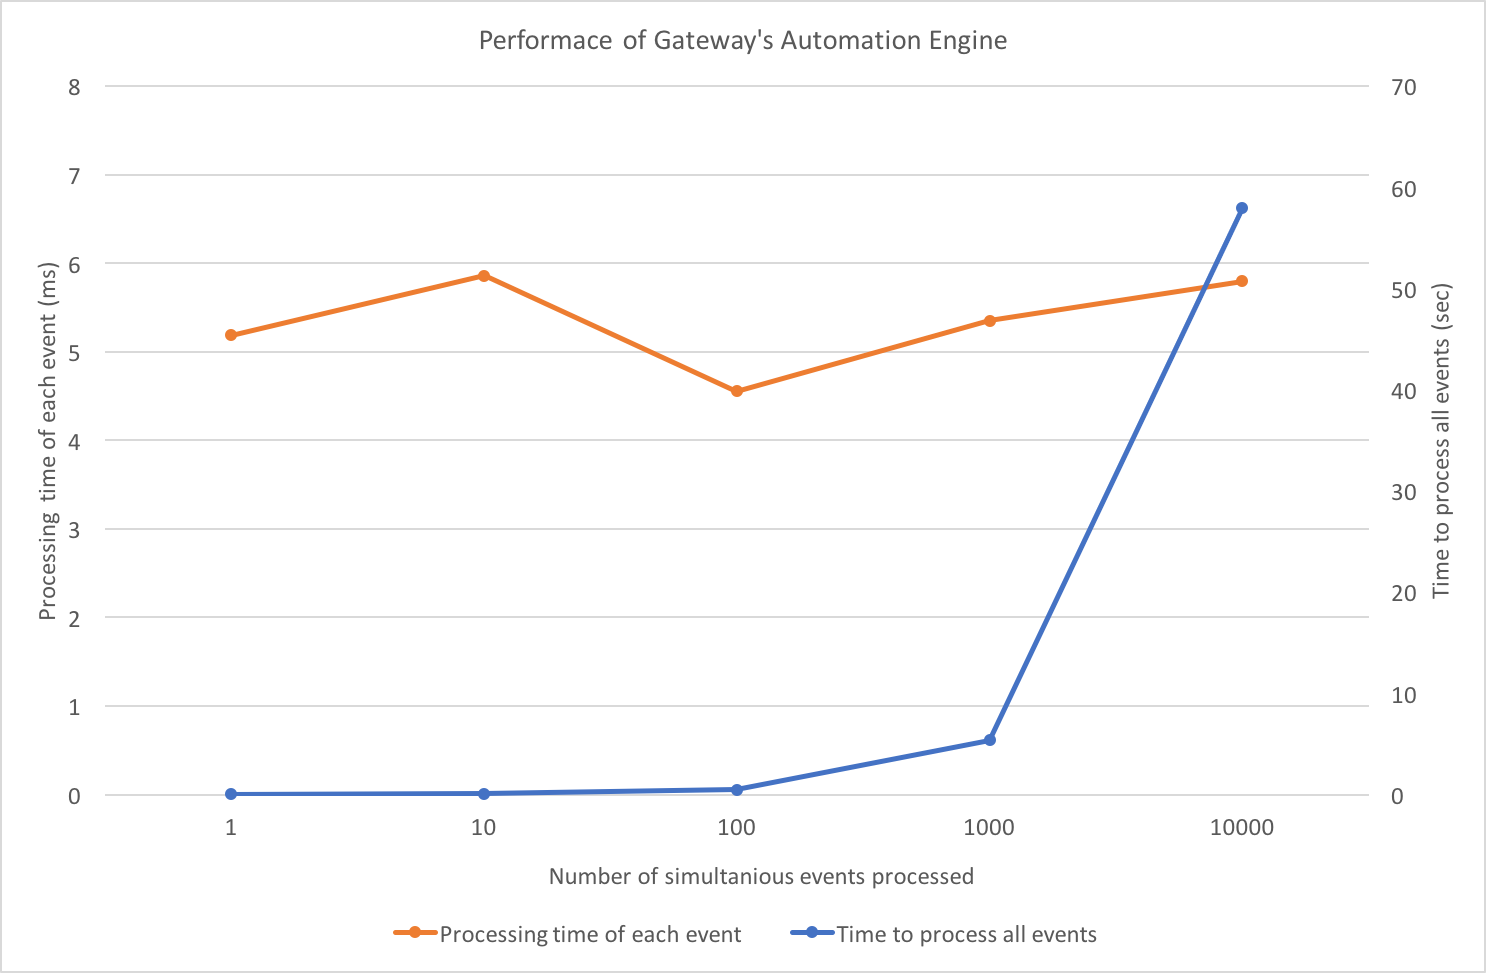
\includegraphics[width=0.9\textwidth]{figures/performance.png}
	\caption{Gateway's Automation Engine Performance.}
	\label{fig:performance}
\end{figure}

\begin{table}[H]
	\centering
	\caption{My caption}
	\label{my-label}
	\begin{tabular}{l|l|l|l|l|l|}
		\cline{2-6}
		& \textbf{1} & \textbf{10} & \textbf{100} & \textbf{1000} & \textbf{10000} \\ \hline
		\multicolumn{1}{|l|}{\textbf{Average Time}}       & 5,2 ms     & 6,9 ms      & 3,7 ms       & 5,3 ms        & 5,8 ms         \\ \hline
		\multicolumn{1}{|l|}{\textbf{Minimum Time}}       & 4,4 ms     & 6,6 ms      & 3,6 ms       & 4,5 ms        & 5,5 ms         \\ \hline
		\multicolumn{1}{|l|}{\textbf{Maximum Time}}       & 6,0 ms     & 7,3 ms      & 3,7 ms       & 6,7 ms        & 6,1 ms         \\ \hline
		\multicolumn{1}{|l|}{\textbf{Standard Deviation}} & 0,7 ms     & 0,3 ms      & 0 ms         & 0,9 ms        & 0,3 ms         \\ \hline
		\multicolumn{1}{|l|}{\textbf{Total Time}}         & 0,005 sec  & 0,069 sec   & 0,367 sec    & 5,350 sec     & 57,953 sec     \\ \hline
	\end{tabular}
	\centering
\caption{Time taken to process each event.}
\label{table:event}
\end{table}

\subsection{System Failure's Reaction Performance}
\label{results:fail}

\begin{table}[H]
	
	\begin{tabular}{|l|l|}
		\hline
		\textbf{Average Time}       & 7,261 sec \\ \hline
		\textbf{Minimum Time}       & 1,185 sec \\ \hline
		\textbf{Maximum Time}       & 5,084 sec \\ \hline
		\textbf{Standard Deviation} & 8,883 sec \\ \hline
	\end{tabular}
	\centering
	\caption{Reaction time to a \ac{cep} Engine failure}
	\label{cepDown}
\end{table}

\begin{table}[H]

	\begin{tabular}{|l|l|}
		\hline
		\textbf{Average Time}       & 13,194 sec \\ \hline
		\textbf{Minimum Time}       & 3,839 sec \\ \hline
		\textbf{Maximum Time}       & 7,492 \\ \hline
		\textbf{Standard Deviation} & 18,877 \\ \hline
	\end{tabular}
	\centering
	\caption{Reaction time to a Gateway failure.}
	\label{gwdown}
\end{table}

\begin{table}[H]
	
	\begin{tabular}{|l|l|}
		\hline
		\textbf{Average Time}       & 0,164 sec \\ \hline
		\textbf{Minimum Time}       & 0,024 sec \\ \hline
		\textbf{Maximum Time}       & 0,129 sec \\ \hline
		\textbf{Standard Deviation} & 0,199 sec \\ \hline
	\end{tabular}
	\centering
	\caption{Reaction time to a Gateway back up.}
	\label{gwup}
\end{table}


Reaction time < 100 ms -> imperceptible 
Miller1968
	\chapter{Conclusions and Future Work}
\label{chapter:conclusions}
	
	
	% End of Thesis text ---------------------------------------------------------
	% Including files is advised:
	
	
	%Appendix
	
	\backmatter
	
	
	%Print all used references
	
	\begingroup
	\renewcommand{\bibfont}{\footnotesize}
	
	%Redefine References name
	\defbibheading{bibliography}[References]{
		\chapter{#1} 
	}
	\SingleSpacing
	\setlength\bibitemsep{8pt}
	\printbibliography[heading=bibliography]
	\endgroup
	
	
	%Load appendix
	%\chapter{Appendix A: \acf{gae} modules code}
\label{chapter:appendix-a}

\begin{listing}[H]
	\begin{minted}[
	frame=single
	]{python}
if self.window != None and self.aggregator != None:

    if self.window._type == 'time':
        if self.aggregator._type == 'any':
            if value is 0:
                return

            event_id = Action.new_event(self)

            Action.apply_converter(self, value, client,r_id, enable)

            await asyncio.sleep(self.window.value)

            if Action.events[self] == event_id:
                Action.apply_converter(self, 0, client, r_id, enable)
	\end{minted}
	\caption{Implementation of the Window Module}
	\label{snippet:rule}
\end{listing}

	
	
\end{document}
